\documentclass[leqno,12pt]{article}
\setlength{\textheight}{23cm}
\setlength{\textwidth}{16cm}
\setlength{\oddsidemargin}{0cm}
\setlength{\evensidemargin}{0cm}
\setlength{\topmargin}{0cm}

\usepackage{amsmath, amssymb}
\usepackage{amsthm}

\usepackage{pdflscape} % Landscape diagram

\def\address#1#2{\begingroup
\noindent\parbox[t]{9cm}{%
\small{\scshape\ignorespaces#1}\par\vskip1ex
\noindent\small{\itshape E-mail address}%
\/: #2\par\vskip4ex}\hfill%
\endgroup}%

\renewcommand{\baselinestretch}{1.2}
\renewcommand{\thefootnote}{}

\theoremstyle{plain}
\newtheorem{theorem}{\indent\sc Theorem}[section]
\newtheorem{lemma}[theorem]{\indent\sc Lemma}
\newtheorem{corollary}[theorem]{\indent\sc Corollary}
\newtheorem{proposition}[theorem]{\indent\sc Proposition}
\newtheorem{claim}[theorem]{\indent\sc Claim}
\newtheorem{conjecture}[theorem]{\indent\sc Conjecture}

\newtheorem{maintheorem}{Theorem}
\renewcommand*{\themaintheorem}{\Roman{maintheorem}}

\theoremstyle{definition}
\newtheorem{definition}[theorem]{\indent\sc Definition}
\newtheorem{remark}[theorem]{\indent\sc Remark}
\newtheorem{example}[theorem]{\indent\sc Example}
\newtheorem{notation}[theorem]{\indent\sc Notation}
\newtheorem{assertion}[theorem]{\indent\sc Assertion}

\newtheorem*{remark0}{\indent\sc Remark}

%%%%% Proof %%%%%
\renewcommand{\proofname}{\indent\sc Proof.}

\pagestyle{myheadings}
\markright{Weil-\'{e}tale cohomology for $n < 0$. Part I: Construction}

\title{\uppercase{Weil-étale cohomology for arbitrary arithmetic schemes and $n < 0$.
  Part I: Construction of Weil-étale complexes}}

\author{\textsc{Alexey Beshenov}}
\date{}

%%%%%%%%%%%%%%%%%%%%%%%%%%%%%%%%%%%%%%%%%%%%%%%%%%%%%%%%%%%%%%%%%%%%%%%%%%%%%%%%

\DeclareMathOperator{\Spec}{Spec}
\DeclareMathOperator{\Gal}{Gal}
\DeclareMathOperator{\Hom}{Hom}
\DeclareMathOperator{\im}{im}
\DeclareMathOperator{\Ext}{Ext}
\DeclareMathOperator{\Tot}{Tot}
\DeclareMathOperator{\coker}{coker}

\newcommand{\NN}{\mathbb{N}}
\newcommand{\ZZ}{\mathbb{Z}}
\newcommand{\QQ}{\mathbb{Q}}
\newcommand{\RR}{\mathbb{R}}
\newcommand{\CC}{\mathbb{C}}
\newcommand{\FF}{\mathbb{F}}

\renewcommand{\div}{\text{\it div}}

\newcommand{\dfn}{\mathrel{\mathop:}=}
\newcommand{\rdfn}{=\mathrel{\mathop:}}

\newcommand{\Wc}{\text{\it W,c}}
\newcommand{\et}{\text{\it \'{e}t}}
\newcommand{\fg}{\text{\it fg}}
\newcommand{\ar}{\text{\it ar}}

\newcommand{\iHom}{\underline{\Hom}}
\newcommand{\RHom}{R\!\Hom}

\usepackage{tikz-cd}
\usetikzlibrary{arrows}
\usetikzlibrary{calc}
\usetikzlibrary{babel}
\usetikzlibrary{decorations.pathreplacing}
\usetikzlibrary{patterns}

\newcommand{\tikzpb}{\ar[phantom,pos=0.2]{dr}{\text{\large$\lrcorner$}}}
\newcommand{\tikzpbur}{\ar[phantom,pos=0.2]{dl}{\text{\large$\llcorner$}}}

%%%%%%%%%%%%%%%%%%%%%%%%%%%%%%%%%%%%%%%%%%%%%%%%%%%%%%%%%%%%%%%%%%%%%%%%%%%%%%%%

\begin{document}

\maketitle

%%%%%%%%%%%%%%% footnote %%%%%%%%%%%%%%%%
\footnote{ %2010 MSC numbers
2010 \textit{Mathematics Subject Classification}.
14F20, 14F42.}
\footnote{ %key words and phrases
  \textit{Key words and phrases}.
  Motivic cohomology, Weil-\'{e}tale cohomology.}

%%%%%%%%%%%%%%%%%%%%%%%%%%%%%%%%%%%%%%%%%

\begin{abstract}
  Flach and Morin constructed in \cite{Flach-Morin-2018} Weil-\'{e}tale
  cohomology $H^i_\Wc (X, \ZZ(n))$ for a proper, regular arithmetic
  scheme $X$ (that is, separated and of finite type over $\Spec \ZZ$) and
  $n \in \ZZ$. In the case when $n < 0$, we generalize their construction to an
  arbitrary arithmetic scheme $X$, thus removing the proper and regular
  assumption. The construction assumes finite generation of suitable \'{e}tale
  motivic cohomology groups.

  This is the first part in a series of two papers. In the present text we
  consider the definition and basic properties of Weil-\'{e}tale cohomology. The
  second part will deal with the conjectural relation of $H^i_\Wc (X, \ZZ(n))$
  with the special value of the zeta function $\zeta (X,s)$ at $s = n < 0$.
\end{abstract}

\section{Introduction}

To a scheme $X$ of finite type over $\Spec \ZZ$ one can attach its
\textbf{zeta function}
$$\zeta (X,s) = \prod_{\substack{x \in X \\ \text{closed pt.}}} \frac{1}{1 - \#\kappa (x)^{-s}}$$
(see e.g. \cite{Serre-1965}). Lichtenbaum envisioned a cohomology theory, known
as \textbf{Weil-\'{e}tale cohomology}, that captures information about the special
value of $\zeta (X,s)$ at $s = n$, namely the vanishing order and corresponding
residue
\cite{Lichtenbaum-2005,Lichtenbaum-2009-number-rings,Lichtenbaum-2009-Euler-char}.
For varieties over finite fields $X/\FF_q$, it was further studied by Geisser
\cite{Geisser-2004,Geisser-2006,Geisser-2010-arithmetic-homology}.
Morin gave in \cite{Morin-2014} a construction for $X \to \Spec\ZZ$ separated,
of finite type, proper, regular, and $n = 0$. This construction was further
generalized by Flach and Morin in \cite{Flach-Morin-2018} to any $n \in \ZZ$,
under the same assumptions on $X$.

The goal of this work is to remove the assumption that $X$ is proper and
regular, and following the ideas from \cite{Flach-Morin-2018}, construct
Weil-\'{e}tale cohomology for any $X$ separated and of finite type over $\Spec\ZZ$
for the case of $n < 0$.

As Flach and Morin already suggest in \cite[Remark 3.11]{Flach-Morin-2018},
we rework all their constructions in terms of Geisser's dualizing cycle
complexes $\ZZ^c (n)$.

For the reader's convenience, this work is split into two parts. The present
Part~I is devoted to the construction of Weil-\'{e}tale complexes
$R\Gamma_\Wc (X, \ZZ (n))$. Their conjectural relation to the special value
of $\zeta (X,s)$ at $s = n$ will be treated in the forthcoming Part~II.

\subsection*{Notation and conventions}

\paragraph{Complexes.}
All the constructions will take place in the derived category of abelian groups
$\mathbf{D} (\ZZ)$. For our needs, we introduce the following terminology.
First recall that a complex of abelian groups $A^\bullet$ is \textbf{perfect} if
it is bounded (i.e. $H^i (A^\bullet) = 0$ for $|i| \gg 0$), and $H^i (A^\bullet)$
are finitely generated abelian groups.

\begin{definition}
  \label{dfn:almost-of-(co)finite-type}
  A complex of abelian groups $A^\bullet$ is \textbf{almost perfect}
  if the cohomology groups $H^i (A^\bullet)$ are finitely generated, and
  bounded, except for possible finite $2$-torsion in arbitrarily high degree.
  That is, $H^i (A^\bullet) = 0$ for $i \ll 0$ and $H^i (A^\bullet)$ is finite
  $2$-torsion for $i \gg 0$.

  An abelian group $A$ is of \textbf{cofinite type} if it is $\QQ/\ZZ$-dual to
  a finitely generated abelian group.

  A complex of abelian groups $A^\bullet$ is of \textbf{cofinite type} if the
  cohomology groups $H^i (A^\bullet)$ are of cofinite type and bounded.

  A complex of abelian groups $A^\bullet$ is \textbf{almost of cofinite type}
  if the cohomology groups $H^i (A^\bullet)$ are of cofinite type and
  bounded, except for possible finite $2$-torsion in arbitrarily high
  degree.
\end{definition}

This terminology is ad hoc and was invented for this text, as such complexes
will appear frequently. Some basic observations about almost perfect and almost
cofinite type complexes are collected in
Appendix~\ref{app:homological-algebra}. We note that this finite $2$-torsion
in arbitrarily high degrees could be removed by working with Artin--Verdier
topology $\overline{X}_\et$ instead of the usual \'{e}tale topology $X_\et$;
see \cite[Appendix~A]{Flach-Morin-2018} for more details. We will not use
Artin--Verdier topology to simplify the exposition, at the cost of some
technical hurdles with $2$-torsion.

\paragraph{\'{E}tale cohomology.}
For an arithmetic scheme $X$ and a complex of \'{e}tale sheaves
$\mathcal{F}^\bullet$, we denote by
\[ R\Gamma (X_\et, \mathcal{F}^\bullet) ~
\text{(resp. }R\Gamma_c (X_\et, \mathcal{F}^\bullet), ~
R\widehat{\Gamma}_c (X_\et, \mathcal{F}^\bullet)\text{)} \]
the complex that calculates the corresponding cohomology, resp. cohomology with
compact support, and modified cohomology with compact support. For convenience
of the reader, the definitions are reviewed in
Appendix~\ref{app:modified-cohomology-with-compact-support}. The purpose of
$R\widehat{\Gamma}_c (X_\et, \mathcal{F}^\bullet)$ is to take care of real
places of $X$. There is a canonical projection
$R\widehat{\Gamma}_c (X_\et, \mathcal{F}^\bullet) \to R\Gamma_c (X_\et, \mathcal{F}^\bullet)$,
which is an isomorphism whenever $X (\RR) = \emptyset$.

\paragraph{Equivariant cohomology.}
We denote by $X (\CC)$ the set of complex points of $X$ equipped with the
analytic topology. It carries the natural action of the Galois group
$G_\RR \dfn \Gal (\CC/\RR)$. For a subring $A \subseteq \RR$ we denote by
$A (n)$ the constant $G_\RR$-equivariant sheaf $(2\pi i)^n \, A$ on
$X (\CC)$. In what follows, we will be interested in $A = \ZZ$, $\QQ$, $\RR$.
For $A = \QQ/\ZZ$ we also consider $\QQ/\ZZ (n) = \QQ (n)/\ZZ (n)$.

In general, a $G$-equivariant sheaf $\mathcal{F}$ on $X (\CC)$ can be defined as
an espace \'{e}tal\'{e} $\pi\colon E\to X (\CC)$ with a $G$-action on $E$ such that the
projection $\pi$ is $G$-equivariant. The equivariant global sections are defined
by $\Gamma (G,X,\mathcal{F}) = \mathcal{F} (X)^G$, with $G$ acting on
$\mathcal{F} (X) = \{ s\colon X\to E \mid \pi\circ s = id_X \}$ via
$(g\cdot s) (x) = g\cdot s (g^{-1}\cdot x)$. Then by definition, the equivariant
cohomology is given by the right derived functors of $\Gamma (G,X,-)$. More
details on $G$-equivariant sheaves can be found in
\cite[Chapitre~2]{Morin-these}. For our modest purposes, it is enough to know
that any $G$-module $A$ gives rise to the corresponding abelian $G$-equivariant
constant sheaf. The latter corresponds to the espace \'{e}tal\'{e}
$X (\CC)\times A \to X (\CC)$, with $A$ equipped with the discrete topology.

There is also a complex of sheaves $\ZZ (n)$ on $X_\et$, defined below in
\ref{dfn:sheaf-Z(n)}. It is not the same as the sheaf
$\ZZ (n) = (2\pi i)^n\,\ZZ$ on $X (\CC)$, but there is no possible confusion,
since these two live in very different topologies. The notation is deliberate,
as we will actually see that the comparison between the \'{e}tale topology on $X$
and analytic topology on $X (\CC)$ relates them
(see proposition~\ref{propn:image-of-Q/Zn-under-alpha}).

\subsection*{Assumptions}

For the purposes of this article, we will call an \textbf{arithmetic scheme} an
arbitrary scheme $X$ that is separated and of finite type over $\Spec \ZZ$.
By $n$ we will always denote a strictly negative integer.

Our construction rests on motivic cohomology, defined in terms of complexes
of \'{e}tale cheaves $\ZZ^c (n)$. These come from Bloch's cycle complexes
\cite{Bloch-1986}, and the reader may also consult Geisser's survey
\cite{Geisser-2005} and \cite{Geisser-2004-Dedekind} for definitions over
$\Spec \ZZ$. Namely, for $i \ge 0$ we consider the algebraic simplex
$\Delta^i = \Spec \ZZ[t_0,\ldots,t_i]/(\sum_i t_i - 1)$, and let $z_n (X,i)$ be
the free abelian group generated by closed integral subschemes
$Z \subset X \times \Delta^i$ of dimension $n + i$ which intersect the faces
properly. Then $z_n (X, \bullet)$ is a (homological) complex of abelian groups,
with differentials given by the alternating sum of intersections with faces.
By definition, $\ZZ^c (n)$ is the (cohomological) complex of \'{e}tale sheaves
$z_n (\text{\textvisiblespace}, -\bullet) [2n]$. For additional details about
$\ZZ^c (n)$, we refer to \cite[\S 2]{Geisser-2010}. To avoid any confusion,
we will use cohomological numbering for all complexes in this paper, and in
particular, we set $H^i (X_\et, \ZZ^c(n)) \dfn H^i (R\Gamma (X_\et, \ZZ^c(n))$.

\vspace{1em}

Now given $X$ and $n$ as above, we state the following conjecture.

\begin{conjecture}
  $\mathbf{L}^c (X_\et,n)$: the cohomology groups $H^i (X_\et, \ZZ^c (n))$ are
  finitely generated for all $i \in \ZZ$.
\end{conjecture}

The conjecture $\mathbf{L}^c (X_\et,n)$ appears in
\cite[Definition~5.8]{Morin-2014}, and it is analogous to the conjecture
$\mathbf{L} (X_\et,d-n)$ in \cite[\S 3.2]{Flach-Morin-2018}. See proposition
\ref{prop:Lc-Xet-n-vs-L-Xet-d-n} for the precise relation of
$\mathbf{L}^c (X_\et,n)$ to other conjectures that appear in the literature.
Our construction of Weil-\'{e}tale complexes $R\Gamma_\Wc (X,\ZZ(n))$ will assume
$\mathbf{L}^c (X_\et,n)$. We refer to \S\ref{sec:known-cases-of-Lc-Xet-n} for
the particular cases when the conjecture is known.

\subsection*{Main results}

Before outlining the construction of Weil-\'{e}tale cohomology, we state the main
results of this paper that make it possible. One of our principal objects is the
following complex of abelian sheaves $\ZZ (n)$ on $X_\et$.

\begin{definition}[{\cite[\S 3.1]{Flach-Morin-2018}}, {\cite[\S 7]{Geisser-2004}}]
  \label{dfn:sheaf-Z(n)}
  Let $X$ be an arithmetic scheme and $n < 0$. For a prime $p$, consider
  the localization $X [1/p]$, and let $\mu_{p^r}$ be the sheaf of $p^r$-th
  roots of unity on $X [1/p]$. We define the twist of $\mu_{p^r}$ by $n$
  as
  $$\mu_{p^r}^{\otimes n} = \iHom_{X[1/p]} (\mu_{p^r}^{\otimes (-n)}, \ZZ/p^r).$$

  Now $\ZZ (n)$ is the complex of sheaves on $X_\et$ given by
  \[ \ZZ (n) = \QQ/\ZZ (n) [-1],
  \quad \text{where }
  \QQ/\ZZ (n) = \bigoplus_p \varinjlim_r j_{p!} \mu_{p^r}^{\otimes n}, \]
  and $j_p$ is the canonical open immersion $X[1/p] \to X$.
\end{definition}

The above sheaves $\ZZ (n)$ should not be confused with cycle complexes;
the latter are $\ZZ^c (n)$ in the setting of this paper.
In \S\ref{sec:arithmetic-duality-theorem} we prove the following arithmetic
duality theorem relating the two.

\begin{maintheorem}
  \label{theorem-I}
  Assuming the conjecture $\mathbf{L}^c (X_\et,n)$, there is a quasi-isomorphism
  of complexes
  \[ R\widehat{\Gamma}_c (X_\et, \ZZ (n)) \xrightarrow{\cong}
  \RHom (R\Gamma (X_\et, \ZZ^c (n)), \QQ/\ZZ [-2]). \]
\end{maintheorem}

The second result we will need is related to the following morphism of
complexes.

\begin{definition}
  \label{dfn:u-infty}
  We define
  $v_\infty^*\colon R\Gamma_c (X_\et, \QQ/\ZZ (n)) \to R\Gamma_c (G_\RR, X (\CC), \QQ/\ZZ (n))$
  as the morphism in the derived category $\mathbf{D} (\ZZ)$ induced by the
  comparison of \'{e}tale and analytic topology
  \[ \Gamma_c (X_\et, \QQ/\ZZ (n)) \to
  \Gamma_c (G_\RR, X (\CC), \alpha^* \QQ/\ZZ (n)) \cong
  \Gamma_c (G_\RR, X (\CC), \QQ/\ZZ (n)) \]
  (see proposition~\ref{prop:inverse-image-gamma} and
  \ref{propn:image-of-Q/Zn-under-alpha}). Then we let
  $u_\infty^*\colon R\Gamma_c (X_\et, \ZZ(n)) \to R\Gamma_c (G_\RR, X (\CC), \ZZ (n))$
  be the composition
  \begin{multline*}
    R\Gamma_c (X_\et, \ZZ(n)) \dfn R\Gamma_c (X_\et, \QQ/\ZZ (n)) [-1]
    \xrightarrow{v_\infty^* [-1]} R\Gamma_c (G_\RR, X (\CC), \QQ/\ZZ (n)) [-1]
    \\ \to R\Gamma_c (G_\RR, X (\CC), \ZZ (n))
  \end{multline*}
  where the last arrow is induced by $\QQ/\ZZ (n) [-1] \to \ZZ (n)$, which comes
  from the distinguished triangle of constant $G_\RR$-equivariant sheaves
  $\ZZ (n) \to \QQ (n) \to \QQ/\ZZ (n) \to \ZZ (n) [1]$.
\end{definition}

Then \S\ref{sec:theorem-II} is devoted to the following result.

\begin{maintheorem}
  \label{theorem-II}
  The morphism $u_\infty^*$ is torsion, i.e. it is a torsion element in the
  abelian group
  $$\Hom_{\mathbf{D} (\ZZ)} (R\Gamma_c (X_\et, \ZZ(n)), R\Gamma_c (G_\RR, X (\CC), \ZZ(n))).$$
\end{maintheorem}

\subsection*{Outline of the construction of Weil-\'{e}tale cohomology}

Here we outline the structure of this paper, as well as our construction of
Weil-\'{e}tale complexes $R\Gamma_\Wc (X, \ZZ (n))$.

First, \S\ref{sec:arithmetic-duality-theorem} is devoted to a proof of
Theorem~\ref{theorem-I}. Some of its consequences are deduced in
\S\ref{sec:consequences-of-theorem-I}. Namely, if we assume the conjecture
$\mathbf{L}^c (X_\et, n)$, then $R\Gamma (X_\et, \ZZ^c (n))$ is an almost
perfect complex, while $R\Gamma_c (X_\et, \ZZ (n))$ is almost of cofinite type
in the sense of Definition~\ref{dfn:almost-of-(co)finite-type}. For this we
first make a little digression in \S\ref{sec:GR-equivariant-cohomology} to
analyze what kind of complexes we obtain for $G_\RR$-equivariant cohomology on
$X (\CC)$.

Theorem~\ref{theorem-I} is used in \S\ref{sec:RGamma-fg} to define a morphism
$\alpha_{X,n}$ in the derived category (see definition~\ref{def:RGamma-fg}),
and declare $R\Gamma_\fg (X, \ZZ(n))$ to be its cone:
\begin{multline*}
  \RHom (R\Gamma (X_\et, \ZZ^c (n)), \QQ [-2]) \xrightarrow{\alpha_{X,n}}
  R\Gamma_c (X_\et, \ZZ (n)) \to
  R\Gamma_\fg (X, \ZZ(n)) \\
  \to \RHom (R\Gamma (X_\et, \ZZ^c (n)), \QQ [-1])
\end{multline*}
The notation \emph{fg} comes from the fact that the complex
$R\Gamma_\fg (X, \ZZ(n))$ is almost perfect in the sense of
Definition~\ref{dfn:almost-of-(co)finite-type}. Thanks to specific properties
of the involved complexes, it turns out that $R\Gamma_\fg (X, \ZZ(n))$ is
defined up to a \emph{unique} isomorphism in the derived category (something one
usually does not expect from a cone).

Then in \S\ref{sec:theorem-II} we establish Theorem~\ref{theorem-II}, and it is
used in \S\ref{sec:RGamma-Wc} to define Weil-\'{e}tale complexes
$R\Gamma_\Wc (X, \ZZ(n))$. For this we deduce from Theorem~\ref{theorem-II} that
$u_\infty^* \circ \alpha_{X,n} = 0$, which implies that there exists a morphism
in the derived category
$$i_\infty^*\colon R\Gamma_\fg (X, \ZZ (n)) \to R\Gamma_c (G_\RR, X (\CC), \ZZ(n))$$
(see the diagram below). We pick a mapping fiber of $i_\infty^*$ and call it
$R\Gamma_\Wc (X, \ZZ (n))$, which turns out to be a perfect complex.
Finally, in \S\ref{sec:known-cases-of-Lc-Xet-n} we consider the cases of $X$ for
which the conjecture $\mathbf{L}^c (X_\et, n)$ is known, and hence our results
hold unconditionally, and in \S\ref{sec:comparison-with-FM} we verify that
whenever $X$ is proper and regular, our complex $R\Gamma_\Wc (X, \ZZ (n))$ is
isomorphic to that constructed in \cite{Flach-Morin-2018}.

There are two appendices to this paper: Appendix~\ref{app:homological-algebra}
collects some lemmas from homological algebra, and
Appendix~\ref{app:modified-cohomology-with-compact-support} reviews the
definitions of \'{e}tale cohomology with compact support $R\Gamma_c (X_\et, -)$
and its modified version $R\widehat{\Gamma}_c (X_\et, -)$.

\vspace{1em}

The definition of $R\Gamma_\Wc (X,\ZZ(n))$ fits in the following commutative
diagram involving distinguished triangles in the derived category
$\mathbf{D} (\ZZ)$:

\[ \begin{tikzcd}[column sep=1em]
    &[-3em] \RHom (R\Gamma (X_\et, \ZZ^c (n)), \QQ [-2]) \ar{d}{\alpha_{X,n}}[swap]{\text{dfn.~\ref{def:RGamma-fg}}} \ar{r} &[-2.5em] 0 \ar{d} \\
    & R\Gamma_c (X_\et, \ZZ(n)) \ar{d}\ar{r}{u_\infty^*} & R\Gamma_c (G_\RR, X (\CC), \ZZ(n))\ar{d}{id} \\
    R\Gamma_\Wc (X, \ZZ (n)) \ar{r} & R\Gamma_\fg (X, \ZZ(n)) \ar[dashed]{r}{i_\infty^*}\ar{d} & R\Gamma_c (G_\RR, X (\CC), \ZZ(n)) \ar{r} \ar{d} & R\Gamma_\Wc (X, \ZZ (n)) [1] \\
    & \RHom (R\Gamma (X_\et, \ZZ^c (n)), \QQ [-1]) \ar{r} & 0
\end{tikzcd} \]

Our construction follows \cite{Flach-Morin-2018}, and in particular,
the resulting complex is the same whenever $X$ is proper and regular, which is
the assumption considered by Flach and Morin. Here is a brief comparison between
the notation.

\begin{center}
  \renewcommand{\arraystretch}{1.5}
  \begin{tabular}{cc}
    \hline
    \textbf{this paper} & \textbf{Flach--Morin} \\
    \hline
    \begin{tabular}{c} cycle complexes \\ $\ZZ^c (n)$ \end{tabular} & \begin{tabular}{c} cycle complexes \\ $\ZZ (d-n)[2d]$, $d = \dim X$ \end{tabular} \\
    \hline
    $R\Gamma_\fg (X, \ZZ(n))$ & \begin{tabular}{c} $R\Gamma_W (\overline{X}, \ZZ(n))$, \\ up to finite $2$-torsion for $i\gg 0$ \end{tabular} \\
    \hline
    $R\Gamma_\Wc (X,\ZZ(n))$ & $R\Gamma_\Wc (X, \ZZ(n))$ \\
    \hline
  \end{tabular}
\end{center}

Further properties of $R\Gamma_\Wc (X, \ZZ (n))$ that are needed to establish
its conjectural relation to the special value of $\zeta (X,s)$ at $s = n$ will
be treated in the second part of this article.

\subsection*{Acknowledgments}

This text is based on the results of my PhD thesis, prepared in Universit\'{e} de
Bordeaux and Universiteit Leiden under supervision of Baptiste Morin and Bas
Edixhoven, and I am deeply grateful for their support during working on this
project. I thank Stephen Lichtenbaum and Niranjan Ramachandran who kindly
accepted to be the referees for my thesis and provided many useful comments and
suggestions. I am also indebted to Matthias Flach, since the ideas of this work
come from \cite{Flach-Morin-2018}. Moreover, the work of Thomas Geisser on
arithmetic duality \cite{Geisser-2010} is also crucial for this paper, and his
work on Weil-\'{e}tale cohomology for varieties over finite fields
\cite{Geisser-2004,Geisser-2006,Geisser-2010-arithmetic-homology} has been of
great influence for me. Finally, I thank Maxim Mornev for various fruitful
conversations. This paper was edited while I was visiting Center for Research
in Mathematics (CIMAT), Guanajuato, Mexico. I am grateful personally to Pedro Luis del
Ángel and Xavier G\'{o}mez Mont for their hospitality.

%%%%%%%%%%%%%%%%%%%%%%%%%%%%%%%%%%%%%%%%%%%%%%%%%%%%%%%%%%%%%%%%%%%%%%%%%%%%%%%%

\section{Proof of Theorem~I}
\label{sec:arithmetic-duality-theorem}

At the heart of our constructions is a certain arithmetic duality theorem for
cycle complexes obtained by Thomas Geisser in \cite{Geisser-2010}. The goal of
this section is to deduce Theorem~\ref{theorem-I} from Geisser's duality.
We would like to establish a quasi-isomorphism of complexes
\[ R\widehat{\Gamma}_c (X_\et, \ZZ (n)) \xrightarrow{\cong}
\RHom (R\Gamma (X_\et, \ZZ^c (n)), \QQ/\ZZ [-2]). \]

Here $R\widehat{\Gamma}_c (X_\et, \ZZ (n))$ denotes the modified \'{e}tale
cohomology with compact support, which is reviewed in the appendix
\ref{app:modified-cohomology-with-compact-support}. We note that
\cite{Geisser-2010} uses the notation ``$R\Gamma_c$'' for our
``$R\widehat{\Gamma}_c$'', but we take extra care to distinguish the two things,
as we will also need the usual \'{e}tale cohomology with compact support
$R\Gamma_c (X_\et, \ZZ (n))$.

We split our proof of Theorem~\ref{theorem-I} in two propositions.

\begin{proposition}
  For any $n < 0$ we have a quasi-isomorphism of complexes
  \begin{equation}
    \label{eqn:duality-quasi-isomorphism-1}
    R\widehat{\Gamma}_c (X_\et, \ZZ (n)) \cong
    \varinjlim_m \RHom (R\Gamma (X_\et, \ZZ/m\ZZ^c (n)), \QQ/\ZZ [-2]).
  \end{equation}

  \begin{proof}
    We unwind our definition of $\ZZ (n)$ for $n < 0$ and reduce everything to
    the results from \cite{Geisser-2010}.

    \vspace{1em}

    As we have
    $\ZZ (n) \dfn \bigoplus_p \varinjlim_r j_{p!} \mu_{p^r}^{\otimes n} [-1]$,
    it will be enough to show that for every prime $p$ and $r=1,2,3,\ldots$
    there is a quasi-isomorphism of complexes
    \[ R\widehat{\Gamma}_c (X_\et, j_{p!} \mu_{p^r}^{\otimes n} [-1]) \cong
    \RHom (R\Gamma (X_\et, \ZZ^c/p^r (n)), \QQ/\ZZ [-2]), \]
    and then pass to the corresponding filtered colimits.

    As in the Definition~\ref{dfn:sheaf-Z(n)}, here $j_p$ denotes the canonical
    open immersion $j_p\colon X[1/p] \hookrightarrow X$. We further denote by
    $f$ the structure morphism $X\to \Spec \ZZ$ and by $f_p$ the structure
    morphism $X [1/p] \to \Spec \ZZ [1/p]$:

    \[ \begin{tikzcd}
      X [1/p]\ar[hookrightarrow]{r}{j_p}\ar{d}[swap]{f_p} & X\ar{d}{f} \\
      \Spec \ZZ [1/p]\ar[hookrightarrow]{r} & \Spec \ZZ
    \end{tikzcd} \]

    As we are going to change the base scheme, let us write $\Hom_X (-,-)$ for
    the $\Hom$ between sheaves on $X_\et$ and $\iHom_X (-,-)$ for the
    internal $\Hom$. Instead of $\Hom_{\Spec R}$, we will simply write
    $\Hom_R$.

    By \cite[Proposition~7.10~(c)]{Geisser-2010}, we have the following
    exchange formulas. If we work with complexes of constructible sheaves on the
    \'{e}tale site of schemes over the spectrum of a number ring
    $\Spec\mathcal{O}$, then for a morphism $\phi$ of such schemes we have
    \begin{align}
      \label{eqn:exchange-formula-1} R \phi_* \mathcal{D} (\mathcal{F}) & \cong \mathcal{D} (R \phi_! \mathcal{F}),\\
      \label{eqn:exchange-formula-2} R \phi^! \mathcal{D} (\mathcal{G}) & \cong \mathcal{D} (\phi^* \mathcal{G}),
    \end{align}
    where the dualization is given by
    \[ \mathcal{D} (\mathcal{F}^\bullet) \dfn
    R\iHom_X (\mathcal{F}^\bullet, \ZZ^c (0)). \]

    Applying the exchange formula \eqref{eqn:exchange-formula-1} to our
    situation, we get
    \begin{equation}
      R\iHom_X (j_{p!} \mu_{p^r}^{\otimes n} [-1], \ZZ^c_X (0)) \cong
      R j_{p*} R\iHom_{X [1/p]} (\mu_{p^r}^{\otimes n} [-1], \ZZ^c_{X [1/p]} (0)).
    \end{equation}

    Using the other exchange formula \eqref{eqn:exchange-formula-2}, we may
    identify
    \begin{align}
      \label{eqn:inverse-image-of-mu} R\iHom_{X [1/p]} (\mu_{p^r}^{\otimes n} [-1], \ZZ^c_{X [1/p]} (0)) & \cong R\iHom_{X[1/p]} (f_p^* \mu_{p^r}^{\otimes n} [-1], \ZZ^c_{X [1/p]} (0)) \\
      \label{eqn:exchange-formula-applied} & \cong R f^!_p R\iHom_{\ZZ [1/p]} (\mu_{p^r}^{\otimes n} [-1], \ZZ^c_{\ZZ [1/p]} (0)) \\
      \label{eqn:identification-of-Zc0-with-Gm} & \cong R f^!_p R\iHom_{\ZZ [1/p]} (\mu_{p^r}^{\otimes n} [-1], \mathbb{G}_\mathrm{m} [1]) \\
      & \cong R f^!_p R\iHom_{\ZZ [1/p]} (\mu_{p^r}^{\otimes n}, \mathbb{G}_\mathrm{m}) [2] \\
      & \cong R f^!_p \mu_{p^r}^{\otimes (1-n)} [2]
    \end{align}

    Here \eqref{eqn:inverse-image-of-mu} simply means that the sheaf
    $\mu_{p^r}^{\otimes n}$ on $X[1/p]$ is the same as the inverse image of the
    corresponding sheaf on $\Spec \ZZ [1/p]$. The quasi-isomorphism
    \eqref{eqn:exchange-formula-applied} is the first exchange formula. Then,
    \eqref{eqn:identification-of-Zc0-with-Gm} is the fact that the complex
    $\ZZ^c_{\ZZ [1/p]} (0)$ is quasi-isomorphic to $\mathbb{G}_\mathrm{m} [1]$
    according to \cite[Lemma~7.4]{Geisser-2010}. Thanks to
    \cite[Theorem 1.2]{Geisser-2004}, we may identify the sheaf
    $\mu_{p^r}^{\otimes (1-n)}$:
    \begin{equation}
      \mu_{p^r}^{\otimes (1-n)} \cong \ZZ_{\ZZ [1/p]}/p^r (1-n) =
      \ZZ^c_{\ZZ [1/p]}/p^r (n) [-2].
    \end{equation}

    Then \cite[Corollary~7.9]{Geisser-2010} tells us that
    \begin{equation}
      R f^!_p \ZZ^c_{\ZZ [1/p]} / p^r (n) \cong \ZZ^c_{X [1/p]} / p^r (n).
    \end{equation}

    Finally, thanks to \cite[Theorem~7.2~(a)]{Geisser-2010} and
    \cite[Proposition~2.3]{Geisser-2010}, we have an isomorphism
    $\ZZ^c_{X [1/p]}/p^r (n) \cong j_p^*\ZZ^c_X/p^r (n)$, and all the above
    gives
    \begin{equation}
      R\iHom_X (j_{p!} \mu_{p^r}^{\otimes n} [-1], \ZZ^c_X (0)) \cong
      R j_{p*} j_p^* \ZZ^c_X/p^r (n) \cong \ZZ^c_X/p^r (n).
    \end{equation}

    After applying $R\Gamma (X_\et, -)$, we get a quasi-isomorphism of
    complexes of abelian groups
    \begin{equation}
      \RHom (j_{p!} \mu_{p^r}^{\otimes n} [-1], \ZZ^c_X (0)) \cong
      R\Gamma (X_\et, \ZZ^c_X/p^r (n)).
    \end{equation}

    Now according to the duality theorem \cite[Theorem 7.8]{Geisser-2010},
    we have
    \begin{equation}
      \RHom (j_{p !} \mu_{p^r}^{\otimes n} [-1], \ZZ^c (0)) \cong
      \RHom (R\widehat{\Gamma}_c (X_\et, j_{p !} \mu_{p^r}^{\otimes n} [-1]), \QQ/\ZZ [-2]).
    \end{equation}

    What we obtain at the end is a quasi-isomorphism
    \[ R\Gamma (X_\et, \ZZ^c/p^r (n)) \cong
    \RHom (R\widehat{\Gamma}_c (X_\et, j_{p !} \mu_{p^r}^{\otimes n} [-1]), \QQ/\ZZ [-2]). \]
    This is almost what we need: if we apply $\RHom (-,\QQ/\ZZ [-2])$, then, as
    $\widehat{H}^i_c (X_\et, j_{p!} \mu_{p^r}^{\otimes n} [-1])$ are
    finite groups (because the sheaves $j_{p!} \mu_{p^r}^{\otimes n}$ are
    constructible), we have
    \begin{multline*}
      \RHom (R\Gamma (X_\et, \ZZ^c/p^r (n)), \QQ/\ZZ[-2]) \cong\\
      \RHom (\RHom (R\widehat{\Gamma}_c (X_\et, j_{p !} \mu_{p^r}^{\otimes n} [-1]), \QQ/\ZZ[-2]), \QQ/\ZZ[-2]) \\
      \cong R\widehat{\Gamma}_c (X_\et, j_{p !} \mu_{p^r}^{\otimes n} [-1]). \qedhere
    \end{multline*}
  \end{proof}
\end{proposition}

Now to conclude the proof of Theorem~\ref{theorem-I}, we identify the complex
on the right hand side of \eqref{eqn:duality-quasi-isomorphism-1}. For this we
will need the conjecture $\mathbf{L}^c (X_\et, n)$.

\begin{proposition}
  \label{prop:a-quasi-isomorphism-with-dirlim}
  Assuming the conjecture $\mathbf{L}^c (X_\et, n)$, there is
  a quasi-isomorphism of complexes
  \[ \varinjlim_m \RHom (R\Gamma (X_\et, \ZZ/m\ZZ^c (n)), \QQ/\ZZ [-2]) \cong
  \RHom (R\Gamma (X_\et, \ZZ^c (n)), \QQ/\ZZ [-2]). \]

  \begin{proof}
    As $\ZZ^c (n)$ is a complex of flat sheaves, the short exact sequence of
    abelian groups
    $$0 \to \ZZ \xrightarrow{\times m} \ZZ \to \ZZ/m\ZZ \to 0$$
    induces a short exact sequence of sheaves
    \begin{equation}
      \label{short-exact-sequence-with-Z/m}
      0 \to \ZZ^c (n) \xrightarrow{\times m} \ZZ^c (n) \to \ZZ/m\ZZ^c (n) \to 0
    \end{equation}

    The morphism $\ZZ^c (n) \to \ZZ/m\ZZ^c (n)$ induces certain morphisms in
    cohomology
    $$H^i (X_\et, \ZZ^c (n)) \to H^i (X_\et, \ZZ/m\ZZ^c (n)).$$
    We claim that if we pass to the duals $\Hom (-, \QQ/\ZZ)$ and then to the
    filtered colimits $\varinjlim_m$, then we obtain an isomorphism.
    (Note that both $\Hom (-, \QQ/\ZZ)$ and $\varinjlim_m$ are exact.)

    The short exact sequence \eqref{short-exact-sequence-with-Z/m} induces
    a long exact sequence in cohomology
    \[ \begin{tikzcd}[column sep=1em,font=\small]
      \cdots\ar{r} & H^i (X_\et, \ZZ^c (n)) \ar{r}{\times m} & H^i (X_\et, \ZZ^c (n))\ar{r} \ar[draw=none]{d}[name=X, anchor=center]{} & H^i (X_\et, \ZZ/m\ZZ^c (n)) \ar[rounded corners,to path={ -- ([xshift=2ex]\tikztostart.east) |- (X.center) \tikztonodes -| ([xshift=-2ex]\tikztotarget.west) -- (\tikztotarget)}]{dll}[at end]{\delta^i} \\
      & H^{i+1} (X_\et, \ZZ^c (n)) \ar{r}{\times m} & H^{i+1} (X_\et, \ZZ^c (n))\ar{r} & H^{i+1} (X_\et, \ZZ/m\ZZ^c (n)) \ar{r} & \cdots
    \end{tikzcd} \]

    We further have exact sequences
    \[ \begin{tikzcd}[row sep=0.8em,column sep=1em,font=\small]
      & & & \ker \delta^i\ar[equal]{d} \\
      & H^i (X_\et, \ZZ^c (n)) \ar{r}{\times m} & H^i (X_\et, \ZZ^c (n))\ar{r} & H^i (X_\et, \ZZ^c (n))_m \ar{r} & 0 \\
      0\ar{r} & {}_m H^{i+1} (X_\et, \ZZ^c (n)) \ar{r} & H^{i+1} (X_\et, \ZZ^c (n))\ar{r}{\times m} & H^{i+1} (X_\et, \ZZ^c (n)) \\
      & \im \delta^i\ar[equal]{u}
    \end{tikzcd} \]
    that give us
    \[ 0 \to H^i (X_\et, \ZZ^c (n))_m \to
    H^i (X_\et, \ZZ/m\ZZ^c (n)) \to
    {}_m H^{i+1} (X_\et, \ZZ^c (n)) \to 0 \]
    Now if we take $\Hom (-,\QQ/\ZZ)$ and filtered colimits $\varinjlim_m$,
    we get
    \begin{multline}
      \label{eqn:short-exact-sequence-with-dirlim}
      0 \to \varinjlim_m \Hom ({}_m H^{i+1} (X_\et, \ZZ^c (n)), \QQ/\ZZ) \to \\
      \varinjlim_m \Hom (H^i (X_\et, \ZZ/m\ZZ^c (n)), \QQ/\ZZ) \to \\
      \varinjlim_m \Hom (H^i (X_\et, \ZZ^c (n))_m, \QQ/\ZZ) \to 0
    \end{multline}

    By the conjecture $\mathbf{L}^c (X_\et, n)$, the group
    $H^{i+1} (X_\et, \ZZ^c (n))$ is finitely generated, and therefore
    the first $\varinjlim_m$ in the short exact sequence
    \eqref{eqn:short-exact-sequence-with-dirlim} vanishes, and we obtain
    isomorphisms
    \[ \varinjlim_m \Hom (H^i (X_\et, \ZZ^c (n))_m, \QQ/\ZZ) \xrightarrow{\cong}
    \varinjlim_m \Hom (H^i (X_\et, \ZZ/m\ZZ^c (n)), \QQ/\ZZ). \]
    It remains to note that the first $\varinjlim_m$ above is canonically
    isomorphic to the complex
    $\Hom (H^i (X_\et, \ZZ^c (n)), \QQ/\ZZ)$, again,
    thanks to finite generation of $H^i (X_\et, \ZZ^c (n))$,
    assuming the conjecture $\mathbf{L}^c (X_\et, n)$.
  \end{proof}
\end{proposition}

%%%%%%%%%%%%%%%%%%%%%%%%%%%%%%%%%%%%%%%%%%%%%%%%%%%%%%%%%%%%%%%%%%%%%%%%%%%%%%%%

\section{$G_\RR$-equivariant cohomology of $X (\CC)$}
\label{sec:GR-equivariant-cohomology}

Given an arithmetic scheme $X$, we consider its complex points $X (\CC)$ equipped
with the usual analytic topology. It carries a natural action of
$G_\RR = \Gal (\CC/\RR)$. We consider $G_\RR$-modules
\[ \ZZ (n) \dfn (2\pi i)^n\,\ZZ, \quad
\QQ (n) \dfn (2\pi i)^n\,\QQ, \quad
\QQ/\ZZ (n) \dfn \QQ (n) / \ZZ (n) \]
as constant $G_\RR$-equivariant sheaves on $X (\CC)$. Then
$R\Gamma_c (X (\CC), A (n))$ (the complex that calculates singular cohomology
with compact support of $X (\CC)$ with coefficients in $A (n)$) is a complex of
$G_\RR$-modules, and we may further take group cohomology (resp. Tate
cohomology), which leads to complexes
\begin{align*}
  R\Gamma_c (G_\RR, X (\CC), A (n)) & \dfn R\Gamma_c (G_\RR, R\Gamma_c (X (\CC), A (n))),\\
  R\widehat{\Gamma}_c (G_\RR, X (\CC), A (n)) & \dfn R\widehat{\Gamma}_c (G_\RR, R\Gamma (X (\CC), A (n))).
\end{align*}
By definition, this is the $G_\RR$-equivariant cohomology (resp. Tate
cohomology) with compact support of $X (\CC)$ with coefficients in $A (n)$.

In this section we analyze what kind of complexes we obtain. All subsequent
lemmas are summarized in the below table.

\begin{center}
  \renewcommand{\arraystretch}{1.5}
  \begin{tabular}{cc}
    \hline
    \textbf{complex} & \textbf{type} \\
    \hline
    $R\Gamma_c (X (\CC), \ZZ (n))$ & perfect \\
    $R\Gamma_c (G_\RR, X (\CC), \ZZ (n))$ & almost perfect \\
    $R\widehat{\Gamma}_c (G_\RR, X (\CC), \ZZ (n))$ & finite $2$-torsion cohomology \\
    \hline
    $R\Gamma_c (X (\CC), \QQ (n))$ & perfect of $\QQ$-vector spaces \\
    $R\widehat{\Gamma}_c (G_\RR, X (\CC), \QQ (n))$ & quasi-isomorphic to $0$ \\
    \hline
    $R\Gamma_c (X (\CC), \QQ/\ZZ (n))$ & cofinite type \\
    $R\Gamma_c (G_\RR, X (\CC), \QQ/\ZZ (n))$ & almost cofinite type \\
    $R\widehat{\Gamma}_c (G_\RR, X (\CC), \QQ/\ZZ (n))$ & finite $2$-torsion cohomology \\
    \hline
  \end{tabular}
\end{center}

First we consider the usual, non-equivariant cohomology. As is well-known, the
complexes $R\Gamma_c (X (\CC), \ZZ)$ are perfect, i.e. the cohomology groups
$H^i_c (X (\CC), \ZZ)$ are finitely generated and zero for $|i| \gg 0$.  The
same is true for $H^i_c (X (\CC), \ZZ (n))$ (here the twist in $\ZZ (n)$ only
changes the $G_\RR$-module structure). For $\QQ/\ZZ$ coefficients, the following
result will be useful.

\begin{lemma}
  \label{lemma:extensions-of-cofinite-type-groups}
  Given an extension of abelian groups
  $0 \to A \to B \to C \to 0$,
  if $A$ and $C$ are of cofinite type, then $B$ is of cofinite type as well.

  \begin{proof}
    For a finitely generated abelian group $G$, denote
    $G^D \dfn \Hom (G, \QQ/\ZZ)$.  We claim that if $G'$ and $G''$ are finitely
    generated abelian groups, then every extension
    $$0 \to G'^D \to E \to G''^D \to 0$$
    is equivalent to the $\QQ/\ZZ$-dual of an extension
    $$0 \to G'' \to G \to G' \to 0$$
    where $G$ is a finitely generated abelian group. In other words,
    we want to show that
    \begin{align*}
      E (G',G'') & \to E (G''^D,G'^D),\\
      [G'' \rightarrowtail G \twoheadrightarrow G'] & \mapsto
      [G'^D \rightarrowtail G^D \twoheadrightarrow G''^D]
    \end{align*}
    is an isomorphism of Yoneda Exts.

    For this we first note that there are isomorphisms of finite groups
    \[ E (G',G'') \cong \Ext_\ZZ^1 (G',G'')
      \quad\text{and}\quad
      E (G''^D, G'^D) \cong \Ext_\ZZ^1 (G''^D, G'^D), \]
    e.g. by considering separately the cases $G', G'' = \ZZ, \ZZ/m\ZZ$ and using
    additivity of $\Ext$. For finitely generated abelian groups, the functor
    $G \rightsquigarrow (G^D)^D$ is the same as profinite completion
    $G \rightsquigarrow \widehat{G} = G\otimes_\ZZ \widehat{\ZZ}$. Therefore,
    the composition
    \[ E (G',G'') \xrightarrow{D}
    E (G''^D,G'^D) \xrightarrow{D}
    E (\widehat{G'},\widehat{G''}) \]
    is an isomorphism.
  \end{proof}
\end{lemma}

\begin{lemma}
  The complex $R\Gamma_c (X (\CC), \QQ/\ZZ (n))$ is of cofinite type.

  \begin{proof}
    The statement follows from the distinguished triangle
    \[ R\Gamma_c (X (\CC), \ZZ) \to
    R\Gamma_c (X (\CC), \ZZ)\otimes_\ZZ \QQ \to
    R\Gamma_c (X (\CC), \QQ/\ZZ) \to
    R\Gamma_c (X (\CC), \ZZ) [1] \]
    Indeed, the associated long exact sequence in cohomology
    \begin{multline*}
      \cdots \to H^i_c (X (\CC), \ZZ) \to
      H^i_c (X (\CC), \ZZ)\otimes_\ZZ \QQ \to
      H^i_c (X (\CC), \QQ/\ZZ) \to\\
      H^{i+1}_c (X (\CC), \ZZ) \to
      H^{i+1}_c (X (\CC), \ZZ)\otimes_\ZZ \QQ \to \cdots
    \end{multline*}
    shows that $H^i_c (X (\CC), \QQ/\ZZ)$ is an extension of a finite group by a
    group of cofinite type:
    \begin{multline*}
      0 \to \coker (H^i_c (X (\CC), \ZZ) \to
      H^i_c (X (\CC), \ZZ)\otimes_\ZZ \QQ) \to\\
      H^i_c (X (\CC), \QQ/\ZZ) \to\\
      \ker (H^{i+1}_c (X (\CC), \ZZ) \to
      H^{i+1}_c (X (\CC), \ZZ)\otimes_\ZZ \QQ) \to 0
    \end{multline*}
    Then according to lemma~\ref{lemma:extensions-of-cofinite-type-groups},
    $H^i_c (X (\CC), \QQ/\ZZ)$ is of cofinite type.

    Finally, $H^i_c (X (\CC), \QQ/\ZZ)$ vanishes for $|i| \gg 0$, because
    $H^i_c (X (\CC), \ZZ)$ does.
  \end{proof}
\end{lemma}

Now we turn to $G_\RR$-equivariant cohomology. In this case we make use of
spectral sequences
\begin{align*}
  E_2^{pq} = H^p (G_\RR, H_c^q (X (\CC), A (n))) & \Longrightarrow H_c^{p+q} (G_\RR, X (\CC), A (n)), \\
  E_2^{pq} = \widehat{H}^p (G_\RR, H_c^q (X (\CC), A (n))) & \Longrightarrow \widehat{H}_c^{p+q} (G_\RR, X (\CC), A (n)).
\end{align*}

Here $H_c^q (X (\CC), A (n)) = 0$ for $q < 0$ and $q \gg 0$. We recall that the
cohomology groups $H^p (G_\RR, H_c^q (X (\CC), A (n)))$ are killed by
$2 = \# G_\RR$ for all $p > 0$; for this see e.g.
\cite[Theorem~6.5.8]{Weibel-1994}. For Tate cohomology, the same argument shows
that $\widehat{H}^p (G_\RR, H_c^q (X (\CC), A (n)))$ are $2$-torsion for all
$p$, including $p = 0$.

\begin{lemma}
  For $A = \QQ$ we have the following.

  \begin{enumerate}
  \item[$1)$] $H^p (G_\RR, H_c^q (X (\CC), \QQ (n))) = 0$ for all $p > 0$,

  \item[$2)$] $\widehat{H}^p (G_\RR, H_c^q (X (\CC), \QQ (n))) = 0$ for all $p$,

  \item[$3)$] $\widehat{H}^p (G_\RR, X (\CC), \QQ (n))) = 0$ for all $p$.
  \end{enumerate}

  \begin{proof}
    The cohomology groups in 1) and 2) are $2$-torsion $\QQ$-vector spaces,
    hence trivial. Part 3) follows from the spectral sequence
    \[ E_2^{pq} = \widehat{H}^p (G_\RR, H^q_c (X (\CC), \QQ (n)))
    \Longrightarrow
    \widehat{H}^{p+q}_c (G_\RR, X (\CC), \QQ (n)). \qedhere \]
  \end{proof}
\end{lemma}

\begin{lemma}
  We have a quasi-isomorphism of complexes
  \[ R\widehat{\Gamma}_c (G_\RR, X (\CC), \QQ/\ZZ (n) [-1]) \cong
  R\widehat{\Gamma}_c (G_\RR, X (\CC), \ZZ (n)).\]

  \begin{proof}
    The short exact sequence of $G_\RR$-equivariant sheaves on $X (\CC)$
    $$0 \to \ZZ (n) \to \QQ (n) \to \QQ/\ZZ (n) \to 0$$
    gives a distinguished triangle
    \begin{multline*}
      R\widehat{\Gamma}_c (G_\RR, X (\CC), \ZZ (n)) \to
      R\widehat{\Gamma}_c (G_\RR, X (\CC), \QQ (n)) \to
      R\widehat{\Gamma}_c (G_\RR, X (\CC), \QQ/\ZZ (n)) \\
      \to R\widehat{\Gamma}_c (G_\RR, X (\CC), \ZZ (n)) [1]
    \end{multline*}
    By the previous lemma, here
    $R\widehat{\Gamma}_c (G_\RR, X (\CC), \QQ (n)) \cong 0$.
  \end{proof}
\end{lemma}

\begin{lemma}
  \label{lemma:H-hat-c-GR-X(C)-Z(n)-finite-2-torsion}
  The groups
  \[ \widehat{H}_c^i (G_\RR, X (\CC), \ZZ (n)) \cong
  \widehat{H}_c^{i-1} (G_\RR, X (\CC), \QQ/\ZZ (n)) \]
  are finite $2$-torsion.

  \begin{proof}
    As we already recalled, $\widehat{H}_c^i (G_\RR, X (\CC), \ZZ (n))$
    are $2$-torsion. To see that the torsion is finite, consider the spectral
    sequence
    \[ E_2^{pq} = \widehat{H}^p (G_\RR, H^q_c (X (\CC), \ZZ (n)))
    \Longrightarrow
    \widehat{H}^{p+q}_c (G_\RR, X (\CC), \ZZ (n)). \]
    The groups $H^q_c (X (\CC), \ZZ (n))$ are finitely generated and vanish for
    $q \gg 0$ and $q < 0$. This means that the second page of the spectral
    sequence looks like

    \begin{center}
      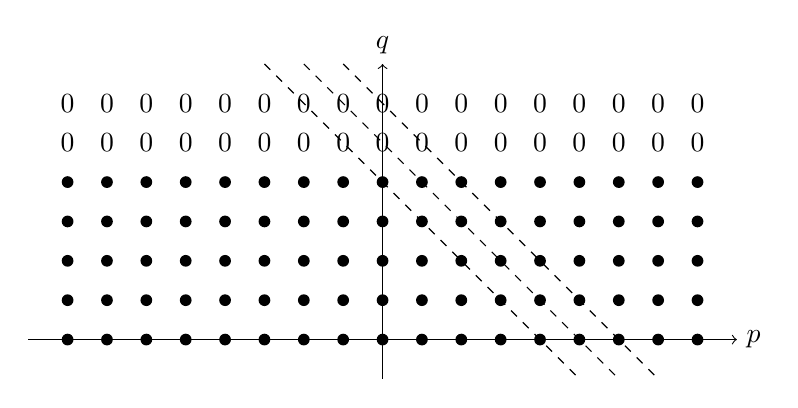
\begin{tikzpicture}[x=0.5cm, y=0.5cm]
        \draw[dashed] (-3,7) -- (5,-1);
        \draw[dashed] (-2,7) -- (6,-1);
        \draw[dashed] (-1,7) -- (7,-1);

        \draw[->] (0,-1) -- (0,7) node[above] {$q$};
        \draw[->] (-9,0) -- (9,0) node[right] {$p$};

        \foreach \p in {-8, ..., 8}
        \foreach \q in {5, ..., 6}
        \draw (\p,\q) node {$0$};

        \foreach \p in {-8, ..., 8}
        \foreach \q in {0, ..., 4}
        \draw (\p,\q) node[circle,fill,inner sep=1.5pt] {};
      \end{tikzpicture}
    \end{center}

    \noindent where all objects are \emph{finite} $2$-torsion.
  \end{proof}
\end{lemma}

\begin{lemma}
  \label{lemma:RGammac(GR,X(C),Z(n))-almost-perfect}
  The complex $R\Gamma_c (G_\RR, X (\CC), \ZZ (n))$
  is almost perfect.

  \begin{proof}
    Similarly, we consider the spectral sequence
    \[ E_2^{pq} = H^p (G_\RR, H^q_c (X (\CC), \ZZ (n)))
    \Longrightarrow
    H^{p+q}_c (G_\RR, X (\CC), \ZZ (n)). \]

    Here $H^p (G_\RR, H^q_c (X (\CC), \ZZ (n)))$ is not necessarily $2$-torsion
    for $p = 0$, and the second page looks like
    \begin{center}
      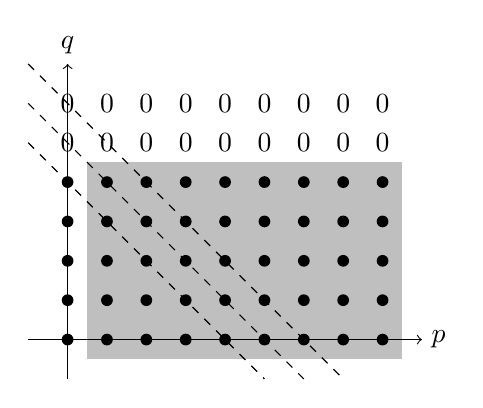
\begin{tikzpicture}[x=0.5cm, y=0.5cm]
        \fill[lightgray] (0.5,-0.5) -- (0.5,4.5) -- (8.5,4.5) -- (8.5,-0.5) -- cycle;

        \draw[dashed] (-1,5) -- (5,-1);
        \draw[dashed] (-1,6) -- (6,-1);
        \draw[dashed] (-1,7) -- (7,-1);

        \draw[->] (0,-1) -- (0,7) node[above] {$q$};
        \draw[->] (-1,0) -- (9,0) node[right] {$p$};

        \foreach \p in {0, ..., 8}
        \foreach \q in {5, ..., 6}
        \draw (\p,\q) node {$0$};

        \foreach \p in {0, ..., 8}
        \foreach \q in {0, ..., 4}
        \draw (\p,\q) node[circle,fill,inner sep=1.5pt] {};
      \end{tikzpicture}
    \end{center}
    where the shaded part $E_2^{pq}$, $p > 0$ consists of finitely generated
    $2$-torsion groups, the line $E_2^{0q}$ consists of finitely generated
    groups, and the objects $E_2^{pq}$ are zero for $q \gg 0$. It follows that
    the groups $H^i (G_\RR, X (\CC), \ZZ (n))$ are all finitely generated as
    well, and they are torsion for $i \gg 0$. This is in fact $2$-torsion, and
    we may see this as follows. If $P_\bullet \twoheadrightarrow \ZZ$ is the
    bar-resolution of $\ZZ$ by free $\ZZ G_\RR$-modules, then the morphism of
    complexes
    \[ \begin{tikzcd}
      \cdots\ar{r} & P_3\ar{r}\ar{d}{2} & P_2\ar{r}\ar{d}{2} & P_1\ar{r}\ar{d}{2} & P_0\ar{r}\ar{d}{2-N} & 0 \\
      \cdots\ar{r} & P_3\ar{r} & P_2\ar{r} & P_1\ar{r} & P_0\ar{r} & 0
    \end{tikzcd} \]
    %% \begin{align*}
    %%   \text{``}2\text{''}\colon P_\bullet & \to P_\bullet,\\
    %%   (2-N)\colon P_0 & \to P_0,\\
    %%   2\colon P_i & \to P_i \quad\text{for }i > 1,
    %% \end{align*}
    which induces multiplication by $2$ on $H^i (G,-)$ for $i > 0$
    is null-homotopic \cite[Theorem 6.5.8]{Weibel-1994}. It is not
    multiplication by $2$ in degree $0$, but as the complex
    $R\Gamma_c (G_\RR, X (\CC), \ZZ (n))$ is bounded, we see that it induces
    multiplication by $2$ on $H^i (G_\RR, X (\CC), \ZZ (n))$ for $i \gg 0$.
  \end{proof}
\end{lemma}

Similarly for $\QQ/\ZZ$-coefficients, we have the following observation.

\begin{lemma}
  \label{lemma:RGammac(GR,X(C),Q/Z(n))-almost-cofinite-type}
  The complex $R\Gamma_c (G_\RR, X (\CC), \QQ/\ZZ (n))$
  is almost of cofinite type.

  \begin{proof}
    Consider the spectral sequence
    \[ E_2^{pq} = H^p (G_\RR, H^q_c (X (\CC), \QQ/\ZZ (n)))
    \Longrightarrow
    H^{p+q} (G_\RR, X (\CC), \QQ/\ZZ (n)). \]

    The second page will have groups of cofinite type on the line $E_2^{0q}$ and
    finite $2$-torsion groups $E_2^{pq}$ for $p > 0$. We have filtrations
    \begin{equation}
      \label{eqn:ss-filtrations}
      H^{p+q} = F^0 (H^{p+q}) \supseteq
      F^1 (H^{p+q}) \supseteq
      F^2 (H^{p+q}) \supseteq \cdots \supseteq
      F^{p+q} (H^{p+q}) \supset F^{p+q+1} (H^{p+q}) = 0
    \end{equation}
    where
    $$0 \to F^{p+1} (H^{p+q}) \to F^p (H^{p+q}) \to E_\infty^{pq} \to 0$$
    Note that $E^{0q}_\infty$ will be groups of cofinite type, and
    $E^{pq}_\infty$ will be finite $2$-torsion groups for $p > 0$, as we are
    going to have
    $$0 \to E_{r+1}^{0q} \to E_r^{0q} \to T \to 0$$
    where $T$ is finite $2$-torsion, and similarly,
    $$E_{r+1}^{pq} \cong \ker d_r^{pq} / \im d_r^{p-r,q+r-1}$$

    \[ E_r^{p-r,q+r-1} \xrightarrow{d_r^{p-r,q+r-1}}
    E_r^{pq} \xrightarrow{d_r^{pq}} E_r^{p+r,q-r+1} \]
    where $E_r^{pq}$ is finite $2$-torsion for $p > 0$. It follows by induction
    that all terms of the filtration \eqref{eqn:ss-filtrations} are finite
    groups, except for $F^0 (H^{p+q}) = H^{p+q}$ itself, which is of cofinite
    type, being an extension of a group of cofinite type $E_\infty^{0q}$ by a
    finite group $F^1 (H^{p+q})$
    (see lemma~\ref{lemma:extensions-of-cofinite-type-groups}). We also see that
    $H^{p+q}$ is $2$-torsion for $p+q \gg 0$.
  \end{proof}
\end{lemma}

\begin{lemma}
  \label{lemma:Tate-vs-normal-cohomology-of-X(C)}
  For $i \ge 2d - 1$ there is an isomorphism of finite $2$-torsion groups
  \[ \widehat{H}^i_c (G_\RR, X (\CC), \ZZ(n)) \cong
    H^i_c (G_\RR, X (\CC), \ZZ(n)). \]

  \begin{proof}
    Consider the spectral sequences
    \begin{align*}
      E^{pq}_2 = \widehat{H}^p (G_\RR, H^q_c (X (\CC), \ZZ(n))) & \Longrightarrow
      \widehat{H}^i_c (G_\RR, X (\CC), \ZZ(n)), \\
      E^{pq}_2 = H^p (G_\RR, H^q_c (X (\CC), \ZZ(n))) & \Longrightarrow
      H^i_c (G_\RR, X (\CC), \ZZ(n)).
    \end{align*}
    Recall that for Tate cohomology one has
    \[ \widehat{H}^p (G_\RR, H^q_c (X (\CC), \ZZ(n))) \cong
      H^p (G_\RR, H^q_c (X (\CC), \ZZ(n)))
      \quad\text{for }p \ge 1. \]
    Further, $H^q_c (X (\CC), \ZZ(n)) = 0$
    for $q \ge 2d-1$, since $X (\CC)$ has topological dimension $\le 2d - 2$
    (assuming $d > 0$, since in case $d = 0$ we have $X (\CC) = \emptyset$, and
    the statement becomes obvious).  Therefore, the spectral sequences look like
    \begin{center}
      \begin{tikzpicture}[x=0.75cm,y=0.75cm]
        \fill[black!20] (-6,0) -- (-6,3) -- (6,3) -- (6,0) -- cycle;
        \fill[pattern=north east lines] (0,0) -- (0,3) -- (6,3) -- (6,0) -- cycle;

        \draw[->] (-6.25,0) -- (6.25,0) node[right] {$p$};
        \draw[->] (0,-1) -- (0,4.5) node[above] {$q$};

        \draw [decorate,decoration={brace,amplitude=10pt}] (-6,0) -- (-6,3) node [black,midway,xshift=-1cm] {$2d - 2$};

        \draw (-1,4.5) -- (4.5,-1) node[below] {$p+q = 2d-1$};
      \end{tikzpicture}
    \end{center}
  \end{proof}
\end{lemma}

%%%%%%%%%%%%%%%%%%%%%%%%%%%%%%%%%%%%%%%%%%%%%%%%%%%%%%%%%%%%%%%%%%%%%%%%%%%%%%%%

\section{Some consequences of Theorem~I}
\label{sec:consequences-of-theorem-I}

\begin{lemma}
  \label{lemma:morphism-hat-Hc(Xet,Z(n))->Hc(Xet,Z(n))}
  The canonical morphism
  $\phi^i\colon \widehat{H}^i_c (X_\et, \ZZ (n)) \to H^i_c (X_\et, \ZZ (n))$
  sits in a long exact sequence
  \begin{multline*}
    \cdots \to \widehat{H}^{i-1}_c (G_\RR, X (\CC), \ZZ (n)) \to
    \widehat{H}_c^i (X_\et, \ZZ(n)) \xrightarrow{\phi^i}
    H_c^i (X_\et, \ZZ(n)) \\
    \to \widehat{H}^i_c (G_\RR, X (\CC), \ZZ (n)) \to \cdots
  \end{multline*}
  where the groups $\widehat{H}^i_c (G_\RR, X (\CC), \ZZ
  (n))$ are finite $2$-torsion. In particular,
  \begin{enumerate}
  \item[$1)$] the kernel and cokernel of $\phi^i$ is finite $2$-torsion,

  \item[$2)$] if $X (\RR) = \emptyset$, then
    $R\widehat{\Gamma}_c (G_\RR, X (\CC), \ZZ (n)) = 0$ and
    $\widehat{H}^i_c (X_\et, \ZZ (n)) \cong H^i_c (X_\et, \ZZ (n))$.
  \end{enumerate}

  \begin{proof}
    The exact sequence follows from the definition of modified \'{e}tale cohomology
    with compact support and Artin's comparison theorem. This is proved in
    \cite[Lemma~6.14]{Flach-Morin-2018}. In particular, the argument shows that
    $R\widehat{\Gamma}_c (G_\RR, X (\CC), \ZZ (n)) \cong
    R\widehat{\Gamma} (G_\RR, v^* Rf_* \ZZ(n))$ where
    $v\colon \Spec \CC \to \Spec \ZZ$ and $f\colon X\to \Spec \ZZ$,
    and $R\widehat{\Gamma}_c (G_\RR, X (\CC), \ZZ (n)) = 0$ if
    $X (\RR) = \emptyset$.

    The fact that $\widehat{H}^i_c (G_\RR, X (\CC), \ZZ (n))$ are finite
    $2$-torsion is our lemma~\ref{lemma:H-hat-c-GR-X(C)-Z(n)-finite-2-torsion}.
  \end{proof}
\end{lemma}

\begin{proposition}
  \label{prop:motivic-cohomology-duality-consequences}
  Let $X$ be an arithmetic scheme of dimension $d$ satisfying the conjecture
  $\mathbf{L}^c (X_\et,n)$ for $n < 0$.

  \begin{enumerate}
  \item[$1)$] If $X (\RR) = \emptyset$, then $H^i (X_\et, \ZZ^c (n)) = 0$ for
    $i > 1$ or $i < -2d$.

  \item[$2)$] In general, $H^i (X_\et, \ZZ^c (n)) = 0$ for $i < -2d$, and
    $H^i (X_\et, \ZZ^c (n))$ is a finite $2$-torsion group for $i > 1$.

  \item[$3)$] If $X/\FF_q$ is a variety over a finite field, then the groups
    $H^i (X_\et, \ZZ^c(n))$ are finite for all $i \in \ZZ$.
  \end{enumerate}

  In general, we have the following cohomology:
  \begin{center}
    \renewcommand{\arraystretch}{1.5}
    \begin{tabular}{ccclcl}
      \hline
      \textbf{groups} & \textbf{type} & $i \ll 0$ & & $i \gg 0$ \\
      \hline
      $H^i (X_\et, \ZZ^c (n))$ & f.g. & $0$ & for $i < -2d$ & $2$-torsion & for $i > 1$ \\
      $\widehat{H}^i_c (X_\et, \ZZ (n))$ & cofinite & $2$-torsion & for $i < 1$ & $0$ & for $i > 2d + 2$ \\
      $H^i_c (X_\et, \ZZ (n))$ & cofinite & $0$ & for $i < 1$ & $2$-torsion & for $i > 2d + 2$ \\
      \hline
    \end{tabular}
  \end{center}
  In particular, $R\Gamma (X_\et, \ZZ^c (n))$ is an almost perfect complex,
  while $R\Gamma_c (X_\et, \ZZ (n))$ is almost of cofinite type in the sense of
  Definition~\ref{dfn:almost-of-(co)finite-type}.

  \begin{proof}
    If $X (\RR) = \emptyset$, then our duality theorem~\ref{theorem-I} gives
    \[ \Hom (H^{2-i} (X_\et, \ZZ^c (n)), \QQ/\ZZ) \cong
      \widehat{H}^i_c (X_\et, \ZZ (n)) \stackrel{X(\RR)=\emptyset}{\cong}
      H^i_c (X_\et, \ZZ (n)). \]
    We have $H^i_c (X_\et, \ZZ (n)) = 0$ for $i < 1$ by the definition of
    $\ZZ (n)$, and $H^i_c (X_\et, \ZZ (n)) = H^{i-1} (X_\et, \QQ/\ZZ(n)) = 0$
    for $i > 2d + 2$ for the reasons of $\ell$-adic cohomological dimension
    \cite[Expos\'{e}~X, Th\'{e}or\`{e}me~6.2]{SGA4}. This proves part 1) of the proposition.

    In part 2), the group $H^i (X_\et, \ZZ^c (n))$ is finite $2$-torsion for
    $i > 1$, thanks to part 1) and
    lemma~\ref{lemma:morphism-hat-Hc(Xet,Z(n))->Hc(Xet,Z(n))}. The fact that
    $H^i (X_\et, \ZZ^c (n)) = 0$ for $i < -2d$ reduces to the case of
    $X (\RR) = \emptyset$ as follows. Consider a finite \'{e}tale covering family
    $\{ U_i \to X \}$, where each $U_i$ is defined over
    $\Spec \mathcal{O}_{F_i}$ for a totally imaginary number field $F_i$.
    We have the Cartan--Leray spectral sequence
    \[ E_1^{p,q} = \bigoplus_{(i_0,\ldots,i_p) \in I^{p+1}} H^q (U_{i_0,\ldots,i_p, \et}, \ZZ^c (n))
      \Longrightarrow H^{p+q} (X_\et, \ZZ^c (n)), \]
    where $U_{i_0,\ldots,i_p} \dfn U_{i_0} \times_X \cdots \times_X U_{i_p}$, and
    $H^q (U_{i_0,\ldots,i_p, \et}, \ZZ^c (n)) = 0$ for $q < -2d$ by part 1).
    It follows that $H^i (X_\et, \ZZ^c (n))$ for $i < -2d$.

    In part 3), the cohomology groups
    $H^i (X_\et, \ZZ (n)) = H^{i-1} (X_\et, \QQ/\ZZ (n))$ are finite for $n < 0$
    by \cite[Theorem~3]{Kahn-2003}.
  \end{proof}
\end{proposition}

\begin{remark}
  If $X$ is proper and regular of dimension $d$, then Beilinson--Soul\'{e}
  vanishing conjecture predicts that
  $H^i (X_\et, \ZZ^c (n)) = H^{i+2d} (X_\et, \ZZ (d-n)) = 0$ for $i < -2d$
  (see for instance \cite[\S 4.3.4]{Kahn-2005}). Therefore, we just proved that
  this is true under the finite generation conjecture $\mathbf{L}^c (X_\et, n)$.
\end{remark}

%%%%%%%%%%%%%%%%%%%%%%%%%%%%%%%%%%%%%%%%%%%%%%%%%%%%%%%%%%%%%%%%%%%%%%%%%%%%%%%%

\section{Complexes $R\Gamma_\fg (X, \ZZ(n))$}
\label{sec:RGamma-fg}

\begin{definition}
  \label{def:RGamma-fg}
  Assuming the conjecture $\mathbf{L}^c (X_\et,n)$, consider a morphism
  $\alpha_{X,n}$ in the derived category $\mathbf{D} (\ZZ)$ given by the
  composition
  \[ \begin{tikzcd}[column sep=4em]
    \RHom (R\Gamma (X_\et, \ZZ^c (n)), \QQ[-2]) \ar{r}{\QQ \twoheadrightarrow \QQ/\ZZ}\ar{ddr}[swap]{\alpha_{X,n}} & \RHom (R\Gamma (X_\et, \ZZ^c (n)), \QQ/\ZZ[-2]) \\
    & R\widehat{\Gamma}_c (X_\et, \ZZ (n)) \ar{u}{\text{Theorem \ref{theorem-I}}}[swap]{\cong} \ar{d}{\text{proj.}} \\
    & R\Gamma_c (X_\et, \ZZ (n))
  \end{tikzcd} \]

  Here the first arrow is induced by the canonical projection $\QQ \to \QQ/\ZZ$,
  and the last arrow is the canonical projection from the modified cohomology
  with compact support to the usual cohomology with compact support
  (see Appendix~\ref{app:modified-cohomology-with-compact-support}).

  We define the complex $R\Gamma_\fg (X, \ZZ(n))$ as a cone of $\alpha_{X,n}$:
  \begin{multline*}
    \RHom (R\Gamma (X_\et, \ZZ^c (n)), \QQ [-2]) \xrightarrow{\alpha_{X,n}}
    R\Gamma_c (X_\et, \ZZ (n)) \to
    R\Gamma_\fg (X, \ZZ(n)) \\
    \to \RHom (R\Gamma (X_\et, \ZZ^c (n)), \QQ [-1])
  \end{multline*}
  Further, we denote
  $$H^i_\fg (X, \ZZ (n)) \dfn H^i (R\Gamma_\fg (X, \ZZ (n))).$$
\end{definition}

\begin{remark}
  \label{rmk:alpha-X-n-determined-by-cohomology}
  Assuming the conjecture $\mathbf{L}^c (X_\et, n)$, the groups
  $H^i_c (X_\et, \ZZ (n))$ are of cofinite type by theorem~\ref{theorem-I},
  while $\RHom (R\Gamma (X_\et, \ZZ^c (n)), \QQ [-2])$ is a complex of
  $\QQ$-vector spaces. Therefore, the morphism $\alpha_{X,n}$ is determined by
  the maps between cohomology groups
  \[ H^i (\alpha_{X,n})\colon
    \Hom (H^{2-i} (X_\et, \ZZ^c (n)), \QQ) \to
    H^i_c (X_\et, \ZZ (n)) \]
  ---see lemma~\ref{lemma:morphisms-in-DAb-between-cplx-of-Q-vs-and-almost-cofinite-type-cplx}.
\end{remark}

\begin{remark}
  We note that our $R\Gamma_\fg (X, \ZZ (n))$ plays the same role as
  $R\Gamma_W (\overline{X}_\et, \ZZ (n))$ that appears in
  \cite[Definition~3.6]{Flach-Morin-2018}. We use a different notation, since
  Flach and Morin work with Artin--Verdier topology, and their complex
  $R\Gamma_W (\overline{X}_\et, \ZZ (n))$ is perfect, while for our complex
  $H^i_\fg (X, \ZZ (n))$ may be finite $2$-torsion in arbitrarily high degree.
\end{remark}

We first note that although the definition might seem complicated at first,
it simplifies if $X$ has no real places.

\begin{proposition}
  \label{prop:RGamma-fg-for-X(R)-empty}
  If $X (\RR) = \emptyset$, then
  \[ R\Gamma_\fg (X, \ZZ (n)) \cong
  \RHom (R\Gamma (X_\et, \ZZ^c (n)), \ZZ [-1]). \]

  \begin{proof}
    In this case
    $R\widehat{\Gamma}_c (X_\et, \ZZ (n)) \to R\Gamma_c (X_\et, \ZZ (n))$
    is the identity morphism, and therefore $\alpha_{X,n}$ sits in the following
    commutative diagram with distinguished columns:
    \[ \begin{tikzcd}
      \RHom (R\Gamma (X_\et, \ZZ^c (n)), \QQ [-2])\ar{d}{\alpha_{X,n}} \ar{r}{\mathrm{id}} & \RHom (R\Gamma (X_\et, \ZZ^c (n)), \QQ [-2])\ar{d} \\
      R\Gamma_c (X_\et, \ZZ (n))\ar{d} \ar{r}{\cong}[swap]{\text{Theorem~\ref{theorem-I}}} & \RHom (R\Gamma (X_\et, \ZZ^c (n)), \QQ/\ZZ [-2])\ar{d} \\
      R\Gamma_\fg (X, \ZZ (n))\ar{d} \ar[dashed]{r}{\cong} & \RHom (R\Gamma (X_\et, \ZZ^c (n)), \ZZ [-1])\ar{d} \\
      \RHom (R\Gamma (X_\et, \ZZ^c (n)), \QQ [-1]) \ar{r}{\mathrm{id}} & \RHom (R\Gamma (X_\et, \ZZ^c (n)), \QQ [-1])
    \end{tikzcd} \]
    Here the first column is our definition of $R\Gamma_\fg (X, \ZZ (n))$,
    and the second column is induced by the distinguished triangle
    $\ZZ \to \QQ \to \QQ/\ZZ \to \ZZ [1]$.
  \end{proof}
\end{proposition}

\begin{proposition}
  \label{prop:RGammafg-almost-perfect}
  Assuming the conjecture $\mathbf{L}^c (X_\et, n)$, the complex
  $R\Gamma_\fg (X, \ZZ (n))$ is almost perfect in the sense of
  {\rm \ref{dfn:almost-of-(co)finite-type}}, i.e. its cohomology groups
  $H^i_\fg (X, \ZZ (n))$ are finitely generated, trivial for $i \ll 0$, and only
  have $2$-torsion for $i \gg 0$.

  \begin{proof}
    By the definition of $R\Gamma_\fg (X, \ZZ (n))$, we have a long exact
    sequence
    \[ \begin{tikzcd}[column sep=1.75em]
      \cdots\ar{r} & \Hom (H^{2-i} (X_\et, \ZZ^c (n)), \QQ) \ar{r}{H^i (\alpha_{X,n})} &[2em] H^i_c (X_\et, \ZZ (n))\ar{r}\ar[draw=none]{d}[name=X, anchor=center]{} & H^i_\fg (X, \ZZ (n)) \ar[rounded corners,to path={ -- ([xshift=2ex]\tikztostart.east) |- (X.center) \tikztonodes -| ([xshift=-2ex]\tikztotarget.west) -- (\tikztotarget)}]{dll}[at end]{\delta^i} \\
      & \Hom (H^{1-i} (X_\et, \ZZ^c (n)), \QQ)\ar{r}{H^{i+1} (\alpha_{X,n})} & H^{i+1}_c (X_\et, \ZZ (n))\ar{r} & \cdots
    \end{tikzcd} \]

    First we observe what happens for $|i| \gg 0$.
    For $i \ll 0$ we have $H^i_c (X_\et, \ZZ (n)) = 0$, and therefore
    $$H^i_\fg (X, \ZZ (n)) \cong \Hom (H^{1-i} (X_\et, \ZZ^c (n)), \QQ) = 0,$$
    since the group $H^{1-i} (X_\et, \ZZ^c (n))$ is torsion by
    proposition~\ref{prop:motivic-cohomology-duality-consequences}.
    Similarly, the complex $R\Gamma (X_\et, \ZZ^c (n))$ is bounded from below by
    proposition~\ref{prop:motivic-cohomology-duality-consequences}, and therefore
    for $i \gg 0$ we have
    $\Hom (H^{2-i} (X_\et, \ZZ^c (n)), \QQ) = 0$, so that
    $H^i_\fg (X, \ZZ (n)) \cong H^i_c (X_\et, \ZZ (n))$, which is finite
    $2$-torsion by proposition~\ref{prop:motivic-cohomology-duality-consequences}.

    Now we consider short exact sequences
    \[ \begin{tikzcd}[row sep=0.5em]
      0 \ar{r} & \ker \delta^i \ar{r}\ar[equals]{d} & H^i_\fg (X, \ZZ (n)) \ar{r} & \im \delta^i \ar{r}\ar[equals]{d} & 0\\
      & \coker H^i (\alpha_{X,n}) & & \ker H^{i+1} (\alpha_{X,n})
    \end{tikzcd} \]

    By the definition of $\alpha_{X,n}$, the morphism $H^i (\alpha_{X,n})$ factors as
    \begin{multline*}
      \Hom (H^{2-i} (X_\et, \ZZ^c (n)), \QQ) \to
      \Hom (H^{2-i} (X_\et, \ZZ^c (n)), \QQ/\ZZ) \xrightarrow{\cong}
      \widehat{H}^i_c (X_\et, \ZZ (n))\\
      \to H^i_c (X_\et, \ZZ (n))
    \end{multline*}

    We recall from lemma~\ref{lemma:morphism-hat-Hc(Xet,Z(n))->Hc(Xet,Z(n))}
    that the morphism
    $\widehat{H}^i_c (X_\et, \ZZ (n)) \to H^i_c (X_\et, \ZZ (n))$ has finite
    $2$-torsion kernel and cokernel.

    The group $H^{2-i} (X_\et, \ZZ^c (n))$ is finitely generated
    according to the conjecture $\mathbf{L}^c (X_\et, n)$. If this
    group is of the form $\ZZ^{\oplus r}\oplus T$, the morphism
    $H^i (\alpha_{X,n})$ is given by
    \[ \QQ^{\oplus r} \twoheadrightarrow
      (\QQ/\ZZ)^{\oplus r} \rightarrowtail
      \widehat{H}^i_c (X_\et, \ZZ (n)) \to
      H^i_c (X_\et, \ZZ (n)) \]
    where
    $(\QQ/\ZZ)^{\oplus r} \rightarrowtail \widehat{H}^i_c (X_\et, \ZZ (n))$ is
    the inclusion of the maximal divisible subgroup in the group of cofinite
    type
    $$\widehat{H}^i_c (X_\et, \ZZ (n)) \cong \Hom (H^{2-i} (X_\et, \ZZ^c (n)), \QQ/\ZZ).$$
    Both kernel and cokernel of the above map are finitely generated, hence
    $H^i_\fg (X, \ZZ (n))$ is finitely generated.
  \end{proof}
\end{proposition}

\begin{proposition}
  \label{prop:RGamma-fg-uniquely-defined}
  The complex $R\Gamma_\fg (X, \ZZ (n))$ is defined up to a unique isomorphism
  in the derived category $\mathbf{D} (\ZZ)$.

  \begin{proof}
    The complex $\RHom (R\Gamma (X_\et, \ZZ^c (n)), \QQ [-2])$ consists of
    $\QQ$-vector spaces, and $R\Gamma_\fg (X, \ZZ (n))$ is almost perfect, so we
    are in the situation of \ref{TR3-TR1-with-uniqueness}.
  \end{proof}
\end{proposition}

\begin{proposition}
  \label{prop:tensoring-RGammafg-with-Z/m-and-Q}
  Assume the conjecture $\mathbf{L}^c (X_\et,n)$ holds and consider the
  distinguished triangle defining $R\Gamma_\fg (X, \ZZ (n))$:
  \begin{multline*}
    \RHom (R\Gamma (X_\et, \ZZ^c (n)), \QQ [-2]) \xrightarrow{\alpha_{X,n}}
    R\Gamma_c (X_\et, \ZZ (n)) \xrightarrow{f}
    R\Gamma_\fg (X, \ZZ (n)) \\
    \xrightarrow{g} \RHom (R\Gamma (X_\et, \ZZ^c (n)), \QQ [-1])
  \end{multline*}

  \begin{enumerate}
  \item[$1)$] The morphism $g$ induces an isomorphism
    \[ g\otimes \QQ\colon R\Gamma_\fg (X, \ZZ (n)) \otimes_\ZZ \QQ \xrightarrow{\cong}
      \RHom (R\Gamma (X_\et, \ZZ^c (n)), \QQ [-1]).\]

  \item[$2)$] For each $m = 1,2,3$ the morphism $f$ induces an isomorphism
    \[ f\otimes \ZZ/m\ZZ\colon
      R\Gamma_c (X_\et, \ZZ (n))\otimes_\ZZ^\mathbf{L} \ZZ/m\ZZ \xrightarrow{\cong}
      R\Gamma_\fg (X, \ZZ (n))\otimes_\ZZ^\mathbf{L} \ZZ/m\ZZ \]
    
  \item[$3)$] For any prime $\ell$ the morphism $f$ induces an isomorphism
    $$\varprojlim_r H_c^i (X_\et, \ZZ/\ell^r (n)) \cong H_\fg^i (X, \ZZ (n)) \otimes_\ZZ \ZZ_\ell.$$
  \end{enumerate}
  
  \begin{proof}
    The cohomology groups $H_c^i (X_\et, \ZZ (n))$ are all torsion, and
    therefore one has $R\Gamma_c (X_\et, \ZZ (n)) \otimes_\ZZ \QQ \cong 0$ in
    the derived category. Similarly, the complexes of $\QQ$-vector spaces
    $\RHom (R\Gamma (X_\et, \ZZ^c (n)), \QQ [\cdots])$ are killed by tensoring
    with $\ZZ/m\ZZ$.  This proves 1) and 2).

    Now 2) implies 3): by finite generation of $H_\fg^i (X, \ZZ (n))$, we have
    \[ \varprojlim_r H_c^i (X_\et, \ZZ/\ell^r (n)) \stackrel{\text{2)}}{\cong}
      \varprojlim_r H_\fg^i (X, \ZZ/\ell^r (n)) \cong
      \varprojlim_r H_\fg^i (X, \ZZ (n))/\ell^r \cong
      H_\fg^i (X, \ZZ (n)) \otimes_\ZZ \ZZ_\ell. \qedhere \]
  \end{proof}
\end{proposition}

The groups $H_\fg^i (X, \ZZ (n))$ provide an integral model for $\ell$-adic
cohomology in the following sense (see also \cite[\S 8]{Geisser-2004}).

\begin{corollary}
  \label{cor:RGamma-fg-model-for-l-adic-cohomology}
  Let $X$ be an arithmetic scheme satisfying the conjecture
  $\mathbf{L}^c (X_\et, n)$ for $n < 0$. Then
  $$H_\fg^i (X, \ZZ (n)) \otimes_\ZZ \ZZ_\ell \cong H^i_c (X [1/\ell]_\et, \ZZ_\ell (n)),$$
  where the right hand side denotes $\ell$-adic cohomology with compact support.

  \begin{proof}
    We have $\ZZ (n)/\ell^r \cong j_{\ell!} \mu_m^{\otimes n}$.
    Now by part 3) of the previous proposition,
    \[ H_\fg^i (X, \ZZ (n)) \otimes_\ZZ \ZZ_\ell \cong
      \varprojlim_r H_c^i (X_\et, j_{\ell!} \mu_{\ell^r}^{\otimes n}) \cong
      \varprojlim_r H_c^i (X [1/\ell]_\et, \mu_{\ell^r}^{\otimes n})
      \stackrel{\text{dfn}}{=} H_c^i (X [1/\ell]_\et, \ZZ_\ell (n)). \qedhere \]
  \end{proof}
\end{corollary}

%%%%%%%%%%%%%%%%%%%%%%%%%%%%%%%%%%%%%%%%%%%%%%%%%%%%%%%%%%%%%%%%%%%%%%%%%%%%%%%%

\section{Proof of Theorem~II}
\label{sec:theorem-II}

The goal of this section is to prove Theorem~\ref{theorem-II}. We recall that it
states that the morphism of complexes $u_\infty^*$, defined as the composition
\[ \begin{tikzcd}
  R\Gamma_c (X_\et, \ZZ(n)) \ar[equals]{d}\ar[dashed]{r}{u_\infty^*} & R\Gamma_c (G_\RR, X (\CC), \ZZ (n)) \\
  R\Gamma_c (X_\et, \QQ/\ZZ (n)) [-1] \ar{r}{v_\infty^* [-1]} & R\Gamma_c (G_\RR, X (\CC), \QQ/\ZZ (n)) [-1] \ar{u}
\end{tikzcd} \]
is torsion. Here the morphism
$v_\infty^*\colon R\Gamma_c (X_\et, \QQ/\ZZ (n)) \to R\Gamma_c (G_\RR, X (\CC), \QQ/\ZZ (n))$
is induced by the comparison functor
$\alpha^*\colon \mathbf{Sh} (X_\et) \to \mathbf{Sh} (G_\RR, X (\CC))$, as
explained in proposition~\ref{prop:inverse-image-gamma}. We first make sure that
$\alpha^*$ identifies the sheaf $\QQ/\ZZ (n)$ on $X_\et$ from
Definition~\ref{dfn:sheaf-Z(n)} with the $G_\RR$-equivariant sheaf
$\QQ/\ZZ (n) \dfn \frac{(2\pi i)^n\,\QQ}{(2\pi i)^n\,\ZZ}$ on $X (\CC)$.

\begin{proposition}
  \label{propn:image-of-Q/Zn-under-alpha}
  For the sheaf $\QQ/\ZZ (n)$ on $X_\et$ we have an isomorphism of
  $G_\RR$-equivariant constant sheaves on $X (\CC)$
  $$\alpha^* \QQ/\ZZ (n) \cong \QQ/\ZZ (n).$$

  \begin{proof}
    First of all, since $\alpha^*$ is the composition of certain inverse image
    functors $\gamma^*$ and $\epsilon^*$ (which are left adjoint) and an
    equivalence of categories $\delta_*$, the functor $\alpha^*$ preserves
    colimits, and in particular
    \begin{equation}
      \label{eqn:alpha-star-commutes-with-colimits}
      \alpha^* \QQ/\ZZ (n) \cong \bigoplus_p \varinjlim_r \alpha^* j_{p!} \mu_{p^r}^{\otimes n}.
    \end{equation}

    Another formal observation is that the base change from $\Spec \ZZ$ to
    $\Spec \CC$ factors through the base change to $\Spec \ZZ [1/p]$, and then
    $j_p^* \circ j_{p!} = id_{\mathbf{Sh} (X [1/p]_\et)}$:
    \[ \begin{tikzcd}
      \mathbf{Sh} (X [1/p]_\et) \ar{r}{j_{p!}}\ar{drr}[swap]{id} & \mathbf{Sh} (X_\et) \ar{rr}{\gamma^*}\ar{dr}{j_p^*} & & \mathbf{Sh} (X_{\CC,\text{\it \'{e}t}}) \\
      & & \mathbf{Sh} (X [1/p]_\et)\ar[dashed]{ur}
    \end{tikzcd} \]
    which means that we may safely erase ``$j_{p!}$'' in
    \eqref{eqn:alpha-star-commutes-with-colimits}, and everything boils down to
    calculating the sheaves
    $$\alpha^* \mu_{p^r}^{\otimes n} = \alpha^* \iHom_{X [1/p]} (\mu_{p^r}^{\otimes (-n)}, \ZZ/p^r \ZZ).$$
    As we base change to $\Spec \CC$, the \'{e}tale sheaf $\mu_{p^r}$ simply becomes
    the constant sheaf $\mu_{p^r} (\CC)$ on $X (\CC)$, and
    $$\alpha^* \mu_{p^r}^{\otimes n} = \iHom_{X (\CC)} (\mu_{p^r}^{\otimes (-n)} (\CC), \ZZ/p^r \ZZ).$$

    Here the twist is given by
    $$\mu_m (\CC)^{\otimes (-n)} \dfn \underbrace{\mu_m (\CC)\otimes\cdots\otimes\mu_m (\CC)}_{-n},$$
    with the $G_\RR$-action on tensor products $A\otimes B$ defined as usual
    by $g\cdot (a\otimes b) = g\cdot a\otimes g\cdot b$, and the
    $G_\RR$-action on $\iHom (A,B)$ being
    $(g\cdot f) (a) \dfn g\cdot f (g^{-1}\cdot a)$.

    What follows are well-known calculations, and we just need to take care of
    the actions of $G_\RR$ and make sure that everything is equivariant. First
    we see that there is a canonical isomorphism of $G_\RR$-modules
    \begin{equation}
      \label{eqn:roots-of-unity-iso-1}
      \mu_m (\CC) \cong \frac{(2\pi i) \, \ZZ}{m\,(2\pi i)\,\ZZ}, \quad
      e^{2\pi i k/m} \mapsto 2\pi i k.
    \end{equation}
    Now there is a $G_\RR$-isomorphism
    \begin{align}
      \label{eqn:roots-of-unity-iso-2}
      \underbrace{(2\pi i)\,\ZZ\otimes\cdots\otimes (2\pi i)\,\ZZ}_{-n} & \xrightarrow{\cong} (2\pi i)^{-n}\,\ZZ,\\
      \notag (2\pi i)\,a_1\otimes\cdots\otimes (2\pi i)\,a_{-n} & \mapsto (2\pi i)^{-n}\,a_1\cdots a_{-n},
    \end{align}
    and combining \eqref{eqn:roots-of-unity-iso-1}
    and \eqref{eqn:roots-of-unity-iso-2}, we obtain
    $$\mu_m (\CC)^{(-n)} \cong \frac{(2\pi i)^{-n} \, \ZZ}{m\,(2\pi i)^{-n}\,\ZZ}.$$
    Finally, we have $G_\RR$-isomorphisms
    \begin{multline*}
      \iHom (\mu_m (\CC)^{(-n)}, \ZZ/m\ZZ) \cong
      \iHom \Bigl(\frac{(2\pi i)^{-n} \, \ZZ}{m\,(2\pi i)^{-n}\,\ZZ}, \ZZ/m\ZZ\Bigr) \\
      \cong
      \iHom ((2\pi i)^{-n}\,\ZZ, \ZZ/m\ZZ) \cong
      \frac{(2\pi i)^n\,\ZZ}{m\,(2\pi i)^n\,\ZZ},
    \end{multline*}
    where the last isomorphism is given by
    $f \mapsto (2\pi i)^n \, f ((2\pi i)^{-n}\cdot 1)$.
    Now
    \[ \alpha^* \ZZ (n) \cong
    \bigoplus_p \varinjlim_r \mu_{p^r} (\CC)^{\otimes n} \cong
    \bigoplus_p \varinjlim_r \frac{(2\pi i)^n\,\ZZ}{p^r\,(2\pi i)^n\,\ZZ} \cong
    \frac{(2\pi i)^n\,\QQ}{(2\pi i)^n\,\ZZ}. \]
    This is a colimit of $G_\RR$-modules, since the transition morphisms are
    $G_\RR$-equivariant.
  \end{proof}
\end{proposition}

We proceed with our proof of Theorem~\ref{theorem-II}. This seems to be rather
nontrivial; our argument (motivated by \cite{Flach-Morin-2018} where it is given
under the assumption that $X$ is proper and regular) will be based on the
following result about $\ell$-adic cohomology.

\begin{proposition}
  \label{prop:l-adic-cohomology-key-lemma}
  Let $f\colon X\to \Spec \ZZ$ be an arithmetic scheme (that is, with $f$
  separated, of finite type) and $n < 0$. Then for any prime $\ell$ we have
  $$(H^i_c (X_{\overline{\QQ},\text{\it \'{e}t}}, \QQ_\ell/\ZZ_\ell (n))^{G_\QQ})_\div = 0.$$

  \begin{proof}
    Let us recall some facts about $\ell$-adic cohomology. We refer to
    \cite[Expos\'{e}~VI]{SGA5} for the details. Let us first consider the sheaf
    $\ZZ_\ell (n)$. It is a
    \textbf{constructible $\ZZ_\ell$-sheaf} (or simply
      \textbf{$\ZZ_\ell$-sheaf} in the terminology of \cite[Rapport]{SGA4-1-2}).
    on $X$ in the sense of \cite[Expos\'{e}~VI, 1.1.1]{SGA5}. We would like to
    compare the cohomology of $\ZZ_\ell (n)$ on
    $X_{\overline{\QQ},\text{\it \'{e}t}}$ and $X_{\overline{\FF_p},\text{\it \'{e}t}}$,
    where $p$ is some prime different from $\ell$, to be determined later.
    For this we fix some algebraic closures $\overline{\QQ}/\QQ$ and
    $\overline{\FF_p}/\FF_p$ and consider the corresponding morphisms
    \[ \overline{\eta}\colon \Spec \overline{\QQ} \to \Spec \ZZ, \quad
    \overline{x}\colon \Spec \overline{\FF_p} \to \Spec \ZZ. \]
    Let $X_{\overline{\QQ},\text{\it \'{e}t}}$ and
    $X_{\overline{\FF_p},\text{\it \'{e}t}}$ be the pullbacks of $X$ along the above
    morphisms:
    \[ \begin{tikzcd}
      X_{\overline{\QQ}} \ar{r}\tikzpb\ar{d}[swap]{f_{\overline{\QQ}}} & X \ar{d}{f} & X_{\overline{\FF_p}} \ar{l}\ar{d}{f_{\overline{\FF_p}}}\tikzpbur \\
      \Spec \overline{\QQ} \ar{r}[swap]{\overline{\eta}} & \Spec \ZZ & \Spec \overline{\FF_p} \ar{l}{\overline{x}}
    \end{tikzcd} \]

    According to \cite[Expos\'{e}~VI, 2.2.3]{SGA5}, the proper base change theorem
    holds for constructible $\ZZ_\ell$-sheaves. It gives us isomorphisms
    \[ H^i_c (X_{\overline{\QQ}, \text{\it \'{e}t}}, \ZZ_\ell (n)) \cong (R^i f_! \ZZ_\ell (n))_{\overline{\eta}}, \quad
    H^i_c (X_{\overline{\FF_p}, \text{\it \'{e}t}}, \ZZ_\ell (n)) \cong (R^i f_! \ZZ_\ell (n))_{\overline{x}}, \]
    where $R^i f_! \ZZ_\ell (n)$ is the same sheaf on $\Spec \ZZ$, and we take
    its different stalks to get cohomology with compact support on different
    fibers. The construction of higher direct images with proper support
    $R^i f_! \mathcal{F}$ for $\ell$-adic sheaves is given in
    \cite[Expos\'{e}~VI, \S 2.2]{SGA5}. The key nontrivial fact that we need is that
    for every morphism (of locally noetherian schemes) $f\colon X\to Y$,
    separated of finite type, if $\mathcal{F}$ is a constructible
    $\ZZ_\ell$-sheaf on $X$, then $R^i f_! \mathcal{F}$ is a constructible
    $\ZZ_\ell$-sheaf on $Y$.

    According to \cite[Expos\'{e}~VI, 1.2.6]{SGA5}, for a projective system of
    abelian sheaves $\mathcal{F} = (\mathcal{F}_n)_{n\in\NN}$ on $X_\et$, the
    following are equivalent:
    \begin{enumerate}
    \item[1)] $\mathcal{F}$ is a constructible $\ZZ_\ell$-sheaf,

    \item[2)] every open subscheme $U\subset X$ is a finite union of locally
      closed pieces $Z_i$ where $\left.\mathcal{F}\right|_{Z_i}$ is a
      \textbf{twisted constant constructible $\ZZ_\ell$-sheaf}
      (or \textbf{faisceau lisse} in the terminology of
      \cite[Rapport]{SGA4-1-2}).
    \end{enumerate}

    Being ``twisted constant'' means that each sheaf $\mathcal{F}_n$ in the
    projective system $(\mathcal{F}_n)_{n\in\NN}$ is locally constant. The
    importance of twisted constant sheaves is explained by the following
    property \cite[Expos\'{e}~VI, 1.2.4, 1.2.5]{SGA5}: for a connected locally
    noetherian scheme $X$, the category of twisted constant
    $\ZZ_\ell$-constructible sheaves on $X$ is equivalent to the category of
    finitely generated $\ZZ_\ell$-modules with a continuous action of the \'{e}tale
    fundamental group $\pi_1^\text{\it \'{e}t} (X)$.

    In our setting, all this means that there exists an open subscheme
    $$U = \Spec \ZZ_S \subset \Spec \ZZ,$$
    where $\ZZ_S$ denotes the localization of $\ZZ$ at a finite set of primes
    $S$, such that the sheaves $R^i f_! \ZZ_\ell (n)$ are twisted constant on
    $U$. By removing the necessary bad primes, we can make sure this holds
    for all $i$.

    Now there exists some prime $p \notin S$ (that is, $(p) \in U$), for which
    we may consider the following picture:
    \[ \begin{tikzcd}
      X_{\overline{\QQ}} \ar{r}\tikzpb\ar{d}[swap]{f_{\overline{\QQ}}} & X_U \ar{d}{f_U} & X_{\overline{\FF_p}} \ar{l}\ar{d}{f_{\overline{\FF_p}}}\tikzpbur \\
      \Spec \overline{\QQ} \ar{r}[swap]{\overline{\eta}} & U & \Spec \overline{\FF_p} \ar{l}{\overline{x}}
    \end{tikzcd} \]

    It follows that we have isomorphisms
    \begin{equation}
      \label{eqn:iso-pbc-Zl-Gal(QS/Q)}
      H^i_c (X_{\overline{\QQ}, \text{\it \'{e}t}}, \ZZ_\ell (n)) \cong (R^i f_{U,!} \ZZ_\ell (n))_{\overline{\eta}} \cong (R^i f_{U,!} \ZZ_\ell (n))_{\overline{x}} \cong H^i_c (X_{\overline{\FF_p}, \text{\it \'{e}t}}, \ZZ_\ell (n)),
    \end{equation}
    of finitely generated $\ZZ_\ell$-modules with continuous action of
    $$\pi_1^\text{\it \'{e}t} (U) \cong \Gal (\QQ_S/\QQ),$$
    where $\QQ_S/\QQ$ denotes a maximal extension of $\QQ$ unramified outside of
    $S$. We note that $(R^i f_{U,!} \ZZ_\ell (n))_{\overline{\eta}}$ naturally
    carries an action of $\pi_1^\text{\it \'{e}t} (U, \overline{\eta})$, while
    $(R^i f_{U,!} \ZZ_\ell (n))_{\overline{x}}$ carries an action of
    $\pi_1^\text{\it \'{e}t} (U, \overline{x})$, and the isomorphism in the middle
    of \eqref{eqn:iso-pbc-Zl-Gal(QS/Q)} sweeps under the rug an identification
    of $\pi_1^\text{\it \'{e}t} (U, \overline{\eta})$ with
    $\pi_1^\text{\it \'{e}t} (U, \overline{x})$.

    To state this more accurately, note that the $\ZZ_\ell$-module
    $H^i_c (X_{\overline{\QQ}, \text{\it \'{e}t}}, \ZZ_\ell (n))$ carries a natural
    action of $G_\QQ$, while
    $H^i_c (X_{\overline{\FF_p}, \text{\it \'{e}t}}, \ZZ_\ell (n))$ carries a
    natural action of $G_{\FF_p}$. After making the necessary choices, we have
    $G_{\QQ_p} \subset G_\QQ$ and a short exact sequence
    $$1 \to I_p \to G_{\QQ_p} \to G_{\FF_p} \to 1$$
    where $I_p$ is the inertia subgroup, acting trivially on
    $H^i_c (X_{\overline{\QQ}, \text{\it \'{e}t}}, \ZZ_\ell (n))$. We have thus
    isomorphisms of finitely generated $\ZZ_\ell$-modules
    \[ H^i_c (X_{\overline{\QQ}, \text{\it \'{e}t}}, \ZZ_\ell (n)) \cong
    H^i_c (X_{\overline{\FF_p}, \text{\it \'{e}t}}, \ZZ_\ell (n)), \]
    equivariant under the action of $G_{\QQ_p}/I_p$ on the left hand side and of
    $G_{\FF_p}$ on the right hand side. To relate all this to $\QQ_\ell (n)$ and
    $\QQ_\ell/\ZZ_\ell (n)$-coefficients, note that we have the following
    isomorphic long exact sequences in cohomology.

    \begin{equation}
      \label{eqn:Zl-Ql-Ql/Zl-les}
      \begin{tikzcd}[column sep=small, font=\small]
        \vdots \ar{d} & \vdots \ar{d} \\
        H_c^{i-1} (X_{\overline{\QQ},\text{\it \'{e}t}}, \QQ_\ell/\ZZ_\ell (n)) \ar{d}{\delta}\ar{r}{\cong} & H_c^{i-1} (X_{\overline{\FF_p},\text{\it \'{e}t}}, \QQ_\ell/\ZZ_\ell (n))  \ar{d}{\delta} \\
        H_c^i (X_{\overline{\QQ},\text{\it \'{e}t}}, \ZZ_\ell (n)) \ar{d}{\phi}\ar{r}{\cong} & H_c^i (X_{\overline{\FF_p},\text{\it \'{e}t}}, \ZZ_\ell (n)) \ar{d}{\phi} \\
        H_c^i (X_{\overline{\QQ},\text{\it \'{e}t}}, \QQ_\ell (n)) \ar{d}{\psi}\ar{r}{\cong} & H_c^i (X_{\overline{\FF_p},\text{\it \'{e}t}}, \QQ_\ell (n)) \ar{d}{\psi} \\
        H_c^i (X_{\overline{\QQ},\text{\it \'{e}t}}, \QQ_\ell/\ZZ_\ell (n)) \ar{r}\ar{d}{\cong} & H_c^i (X_{\overline{\FF_p},\text{\it \'{e}t}}, \QQ_\ell/\ZZ_\ell (n)) \ar{d} \\
        \vdots & \vdots \\
      \end{tikzcd}
\end{equation}

    Here
    \begin{align*}
      H_c^i (X_{\overline{\QQ},\text{\it \'{e}t}}, \QQ_\ell (n)) & = H_c^i (X_{\overline{\QQ},\text{\it \'{e}t}}, \ZZ_\ell (n))\otimes_{\ZZ_\ell} \QQ_\ell,\\
      H_c^i (X_{\overline{\FF_p},\text{\it \'{e}t}}, \QQ_\ell (n)) & = H_c^i (X_{\overline{\FF_p},\text{\it \'{e}t}}, \ZZ_\ell (n))\otimes_{\ZZ_\ell} \QQ_\ell,
    \end{align*}
    and the arrows $\phi$ above are canonical localization morphisms.
    The horizontal arrows are equivariant isomorphisms in the above sense. Note
    that we have
    \[ H^i_c (X_{\overline{\QQ}, \text{\it \'{e}t}}, \QQ_\ell/\ZZ_\ell (n))^{G_\QQ} \rightarrowtail
    H^i_c (X_{\overline{\QQ}, \text{\it \'{e}t}}, \QQ_\ell/\ZZ_\ell (n))^{G_{\QQ_p}/I_p}
    \cong H^i_c (X_{\overline{\FF_p}, \text{\it \'{e}t}}, \QQ_\ell/\ZZ_\ell (n))^{G_{\FF_p}}, \]
    so in order to prove that
    $$(H^i_c (X_{\overline{\QQ},\text{\it \'{e}t}}, \QQ_\ell/\ZZ_\ell (n))^{G_\QQ})_\div = 0,$$
    it will be enough to show that
    $$(H^i_c (X_{\overline{\FF_p},\text{\it \'{e}t}}, \QQ_\ell/\ZZ_\ell (n))^{G_{\FF_p}})_\div = 0.$$
    From now on we move to the characteristic $p$ and consider the fixed points
    of $G_{\FF_p}$ acting on the $\ZZ_\ell$-module
    $H^i_c (X_{\overline{\FF_p},\text{\it \'{e}t}}, \QQ_\ell/\ZZ_\ell (n))$.
    In the long exact sequence \eqref{eqn:Zl-Ql-Ql/Zl-les}, we have (keeping in
    mind that $\phi$ is merely the localization morphism):
    \begin{align*}
      \ker \phi & = H^i_c (X_{\overline{\FF_p},\text{\it \'{e}t}}, \ZZ_\ell (n))_{tor},\\
      \ker \psi & = \im \phi \cong H^i_c (X_{\overline{\FF_p},\text{\it \'{e}t}}, \ZZ_\ell (n)) / \ker \phi \\
      & \quad\quad\quad = \frac{H^i_c (X_{\overline{\FF_p},\text{\it \'{e}t}}, \ZZ_\ell (n))}{H^i_c (X_{\overline{\FF_p},\text{\it \'{e}t}}, \ZZ_\ell (n))_{tor}} \rdfn H^i_c (X_{\overline{\FF_p},\text{\it \'{e}t}}, \ZZ_\ell (n))_{cotor},\\
      \im \psi & = H_c^i (X_{\overline{\FF_p},\text{\it \'{e}t}}, \QQ_\ell/\ZZ_\ell (n))_\div.
    \end{align*}

    This gives us a short exact sequence
    \[ 0 \to H^i_c (X_{\overline{\FF_p},\text{\it \'{e}t}}, \ZZ_\ell (n))_{cotor} \to
    H^i_c (X_{\overline{\FF_p},\text{\it \'{e}t}}, \QQ_\ell (n)) \to
    H^i_c (X_{\overline{\FF_p},\text{\it \'{e}t}}, \QQ_\ell/\ZZ_\ell (n))_\div \to 0 \]
    After taking the $G_{\FF_p}$-invariants, we obtain a long exact sequence
    of cohomology groups
    \begin{multline}
      \label{eqn:cohomology-long-exact-sequence-with-GFp}
      0 \to (H^i_c (X_{\overline{\FF_p},\text{\it \'{e}t}}, \ZZ_\ell (n))_{cotor})^{G_{\FF_p}} \to
      H^i_c (X_{\overline{\FF_p},\text{\it \'{e}t}}, \QQ_\ell (n))^{G_{\FF_p}} \\
      \to (H^i_c (X_{\overline{\FF_p},\text{\it \'{e}t}}, \QQ_\ell/\ZZ_\ell (n))_\div)^{G_{\FF_p}} \to
      H^1 (G_{\FF_p}, H^i_c (X_{\overline{\FF_p},\text{\it \'{e}t}}, \ZZ_\ell (n))_{cotor}) \to \cdots
    \end{multline}

    We claim that
    \begin{equation}
      \label{eqn:SGA-7-expose-XXI-5-5-3}
      H^i_c (X_{\overline{\FF_p},\text{\it \'{e}t}}, \QQ_\ell (n))^{G_{\FF_p}} = 0.
    \end{equation}

    Indeed, according to \cite[Expos\'{e}~XXI, 5.5.3]{SGA7}, the eigenvalues of the
    geometric Frobenius acting on
    $H^i_c (X_{\overline{\FF_p},\text{\it \'{e}t}}, \QQ_\ell)$ are algebraic
    integers. We are twisting $\QQ_\ell$ by $n$, so the eigenvalues of Frobenius
    lie in $p^{-n}\,\overline{\ZZ}$. Since $n < 0$ by our assumption, this
    implies that $1$ does not occur as an eigenvalue.

    Now \eqref{eqn:SGA-7-expose-XXI-5-5-3} and the long exact sequence
    \eqref{eqn:cohomology-long-exact-sequence-with-GFp} imply that there is a
    monomorphism
    \[ (H^i_c (X_{\overline{\FF_p},\text{\it \'{e}t}}, \QQ_\ell/\ZZ_\ell (n))_\div)^{G_{\FF_p}} \rightarrowtail
    H^1 (G_{\FF_p}, H^i_c (X_{\overline{\FF_p},\text{\it \'{e}t}}, \ZZ_\ell (n))_{cotor}), \]
    which restricts to a monomorphism between the maximal divisible subgroups
    \[ ((H^i_c (X_{\overline{\FF_p},\text{\it \'{e}t}}, \QQ_\ell/\ZZ_\ell (n))_\div)^{G_{\FF_p}})_\div \rightarrowtail
    H^1 (G_{\FF_p}, H^i_c (X_{\overline{\FF_p},\text{\it \'{e}t}}, \ZZ_\ell (n))_{cotor})_\div. \]
    However,
    $H^1 (G_{\FF_p}, H^i_c (X_{\overline{\FF_p},\text{\it \'{e}t}}, \ZZ_\ell (n))_{cotor})$
    is a finitely generated $\ZZ_\ell$-module, and therefore its
    maximal divisible subgroup is trivial. We have therefore
    \[ (H^i_c (X_{\overline{\FF_p},\text{\it \'{e}t}}, \QQ_\ell/\ZZ_\ell (n))^{G_{\FF_p}})_\div =
    ((H^i_c (X_{\overline{\FF_p},\text{\it \'{e}t}}, \QQ_\ell/\ZZ_\ell (n))_\div)^{G_{\FF_p}})_\div = 0. \]
    (For the first equality, note that for any $G$-module $A$ one has
    $((A_\div)^G)_\div = (A^G)_\div$.)
  \end{proof}
\end{proposition}

\begin{proof}[Proof of Theorem~\ref{theorem-II}]
  By Definition~\ref{dfn:u-infty}, this amounts to showing that the morphism
  $$v_\infty^*\colon R\Gamma_c (X_\et, \QQ/\ZZ (n)) \to R\Gamma_c (G_\RR, X (\CC), \QQ/\ZZ (n))$$
  is torsion. The complexes $R\Gamma_c (X_\et, \QQ/\ZZ (n))$ and
  $R\Gamma_c (G_\RR, X (\CC), \QQ/\ZZ (n))$ are almost of cofinite type by
  proposition~\ref{prop:motivic-cohomology-duality-consequences} and
  lemma~\ref{lemma:RGammac(GR,X(C),Q/Z(n))-almost-cofinite-type} respectively.
  Therefore, according to \ref{lemma:torsion-morphisms-in-D(Z)}, to show that
  $v^*_\infty\colon R\Gamma_c (X_\et, \QQ/\ZZ (n)) \to R\Gamma_c (G_\RR, X
  (\CC), \QQ/\ZZ (n))$ is torsion in $\mathbf{D} (\ZZ)$, it is enough to show
  that the corresponding morphisms on the maximal divisible subgroups
  \[ H^i_c (v^*_\infty)_\div\colon H^i_c (X_\et, \QQ/\ZZ (n))_\div \to
     H^i_c (G_\RR, X (\CC), \QQ/\ZZ (n))_\div \]
  are all trivial. The morphism $H^i_c (v^*_\infty)$ factors through
  $H^i_c (X_{\overline{\QQ}, \text{\it \'{e}t}}, \mu^{\otimes n})^{G_\QQ}$, where
  $\mu^{\otimes n}$ is the sheaf of all roots of unity on
  $X_{\overline{\QQ}, \text{\it \'{e}t}}$ twisted by $n$.
  We have therefore
  \[ \begin{tikzcd}[column sep=0pt]
    H^i_c (X_\et, \QQ/\ZZ (n))_\div\ar{rr}{H^i_c (v^*_\infty)_\div}\ar[dashed]{dr} && H^i_c (G_\RR, X (\CC), \QQ/\ZZ (n))_\div\\
    & \left(H^i_c (X_{\overline{\QQ}, \text{\it \'{e}t}}, \mu^{\otimes n})^{G_\QQ}\right)_\div\ar[dashed]{ur}
  \end{tikzcd} \]
  Now
  \begin{multline*}
    \left(H^i_c (X_{\overline{\QQ}, \text{\it \'{e}t}}, \mu^{\otimes n})^{G_\QQ}\right)_\div \cong
    \left(\bigoplus_\ell H^i_c (X_{\overline{\QQ}, \text{\it \'{e}t}}, \QQ_\ell/\ZZ_\ell (n))^{G_\QQ}\right)_\div \\
    \cong
    \bigoplus_\ell \left(H^i_c (X_{\overline{\QQ}, \text{\it \'{e}t}}, \QQ_\ell/\ZZ_\ell (n))^{G_\QQ}\right)_\div,
  \end{multline*}
  where all summands are trivial according to
  \ref{prop:l-adic-cohomology-key-lemma}.
\end{proof}

%%%%%%%%%%%%%%%%%%%%%%%%%%%%%%%%%%%%%%%%%%%%%%%%%%%%%%%%%%%%%%%%%%%%%%%%%%%%%%%%

\section{Weil-\'{e}tale complexes $R\Gamma_\Wc (X, \ZZ(n))$}
\label{sec:RGamma-Wc}

The goal of this section is to construct Weil-\'{e}tale cohomology complexes
$R\Gamma_\Wc (X, \ZZ(n))$.

\begin{lemma}
  Let $X$ be an arithmetic scheme and $n < 0$. Assume the conjecture
  $\mathbf{L}^c (X_\et, n)$, so that the morphism $\alpha_{X,n}$ exists.
  Then $u_\infty^* \circ \alpha_{X,n} = 0$.

  \[ \begin{tikzcd}
    \RHom (R\Gamma (X, \ZZ^c (n)), \QQ [-2]) \ar{d}[swap]{\alpha_{X,n}}\ar{dr}{= 0} \\
      R\Gamma_c (X_\et, \ZZ (n)) \ar{r}{u_\infty^*} & R\Gamma_c (G_\RR, X (\CC), \ZZ (n))
    \end{tikzcd} \]

  \begin{proof}
    The morphism $\alpha_{X,n}$ is defined on a complex of $\QQ$-vector spaces,
    and $u_\infty^*$ is torsion by Theorem~\ref{theorem-II}.
  \end{proof}
\end{lemma}

\begin{definition}
  \label{dfn:i-infty}
  We let
  $i_\infty^*\colon R\Gamma_\fg (X, \ZZ (n)) \to R\Gamma_c (G_\RR, X (\CC), \ZZ (n))$
  be a morphism in $\mathbf{D} (\ZZ)$ that gives a morphism of distinguished
  triangles
  \begin{equation}
    \label{eqn:triangle-defining-i-infty}
    \begin{tikzcd}
      \RHom (R\Gamma (X, \ZZ^c (n)), \QQ [-2]) \ar{d}[swap]{\alpha_{X,n}}\ar{r} & 0\ar{d} \\
      R\Gamma_c (X_\et, \ZZ (n)) \ar{r}{u_\infty^*}\ar{d} &  R\Gamma_c (G_\RR, X (\CC), \ZZ (n)) \ar{d}{id} \\
      R\Gamma_\fg (X, \ZZ (n)) \ar[dashed]{r}{i_\infty^*}\ar{d} & R\Gamma_c (G_\RR, X (\CC), \ZZ (n)) \ar{d} \\
      \RHom (R\Gamma (X, \ZZ^c (n)), \QQ [-1])\ar{r} & 0 \\
    \end{tikzcd}
  \end{equation}
\end{definition}

\begin{proposition}
  \label{prop:uniqueness-of-i-infty}
  The morphism $i_\infty^*$ is uniquely defined.

  \begin{proof}
    We may apply \ref{TR3-TR1-with-uniqueness}, since
    $\RHom (R\Gamma (X, \ZZ^c (n)), \QQ [-2])$ is a complex of $\QQ$-vector
    spaces, and both
    $R\Gamma_\fg (X, \ZZ (n))$ and
    $R\Gamma_c (G_\RR, X (\CC), \ZZ (n))$
    are almost perfect complexes by
    proposition~\ref{prop:RGammafg-almost-perfect} and
    lemma~\ref{lemma:RGammac(GR,X(C),Z(n))-almost-perfect}.
  \end{proof}
\end{proposition}

\begin{proposition}
  \label{i-infty-is-torsion}
  The morphism $i_\infty^*$ is torsion in the derived category,
  i.e. we have $i_\infty^*\otimes \QQ = 0$.

  \begin{proof}
    Let us examine the morphism of distinguished triangles
    \eqref{eqn:triangle-defining-i-infty} that defines $i_\infty^*$; in
    particular, the commutative diagram
    \[ \begin{tikzcd}
      R\Gamma_c (X_\et, \ZZ (n)) \ar{r}\ar{d}[swap]{u_\infty^*} & R\Gamma_\fg (X, \ZZ (n))\ar{dl}{i_\infty^*} \\
      R\Gamma_c (G_\RR, X (\CC), \ZZ (n))
    \end{tikzcd} \]

    According to \ref{TR3-TR1-with-uniqueness}, the morphism
    \begin{multline*}
      \Hom_{\mathbf{D} (\ZZ)} (R\Gamma_\fg (X,\ZZ (n)), R\Gamma_c (G_\RR, X (\CC), \ZZ (n))) \\
      \to
      \Hom_{\mathbf{D} (\ZZ)} (R\Gamma_c (X_\et, \ZZ (n)), R\Gamma_c (G_\RR, X (\CC), \ZZ (n)))
    \end{multline*}
    induced by the composition with
    $R\Gamma_c (X_\et, \ZZ (n)) \to R\Gamma_\fg (X,\ZZ (n))$, is mono, and
    therefore
    \begin{multline*}
      \Hom_{\mathbf{D} (\ZZ)} (R\Gamma_\fg (X,\ZZ (n)), R\Gamma_c (G_\RR, X (\CC), \ZZ (n)))\otimes_\ZZ \QQ \to\\
      \Hom_{\mathbf{D} (\ZZ)} (R\Gamma_c (X_\et, \ZZ (n)), R\Gamma_c (G_\RR, X (\CC), \ZZ (n)))\otimes_\ZZ \QQ
    \end{multline*}
    is mono as well. However, $u_\infty^*\otimes \QQ = 0$ by
    Theorem~\ref{theorem-II}, and this implies that $i_\infty^*\otimes \QQ = 0$.
  \end{proof}
\end{proposition}

Now we are ready to define Weil-\'{e}tale complexes.

\begin{definition}
  \label{dfn:RGammaWc}
  We let
  $R\Gamma_\Wc (X,\ZZ(n))$ be an object in the derived category
  $\mathbf{D} (\ZZ)$ which is a mapping fiber of $i_\infty^*$:
  \[ R\Gamma_\Wc (X,\ZZ(n)) \to
  R\Gamma_\fg (X, \ZZ (n)) \xrightarrow{i_\infty^*}
  R\Gamma_c (G_\RR, X (\CC), \ZZ (n)) \to
  R\Gamma_\Wc (X,\ZZ(n)) [1] \]
  The \textbf{Weil-\'{e}tale cohomology with compact support} is given by
  $$H_\Wc^i (X, \ZZ (n)) \dfn H^i (R\Gamma_\Wc (X,\ZZ(n))).$$
\end{definition}

\begin{remark}
  Note that this defines $R\Gamma_\Wc (X,\ZZ(n))$ up to a non-unique isomorphism
  in $\mathbf{D} (\ZZ)$, and the groups $H_\Wc^i (X, \ZZ (n))$ are also defined
  up to a non-unique isomorphism. In a continuation of this paper we will make
  use of the determinant $\det\nolimits_\ZZ R\Gamma_\Wc (X,\ZZ(n))$ (in the
  sense of \cite{Knudsen-Mumford-1976}), which will be defined up to a canonical
  isomorphism.

  Nevertheless, we recall from proposition~\ref{prop:RGamma-fg-uniquely-defined}
  that $R\Gamma_\fg (X, \ZZ (n))$ is defined up to a unique isomorphism in the
  derived category $\mathbf{D} (\ZZ)$. If we could define
  $i_\infty^*\colon R\Gamma_\fg (X, \ZZ(n)) \to R\Gamma_c (G_\RR, X(\CC), \ZZ(n))$
  as an explicit, genuine morphism of complexes (not merely a morphism in the
  derived category $\mathbf{D} (\ZZ)$), this would give us a canonical and
  functorial definition for $R\Gamma_\Wc (X, \ZZ(n))$.
\end{remark}

\subsection*{Case of varieties over finite fields}

For varieties over finite fields, our Weil-\'{e}tale cohomology has a simple
description, and it is $\QQ/\ZZ$-dual to the arithmetic homology studied by
Geisser in \cite{Geisser-2010-arithmetic-homology}.

\begin{proposition}
  If $X$ is a variety over a finite field $\FF_q$, then assuming
  $\mathbf{L}^c (X,n)$, there is an isomorphism of complexes
  \begin{equation}
    \label{eqn:RGamma-Wc-over-finite-fields}
    R\Gamma_\Wc (X,\ZZ(n)) \cong \RHom (R\Gamma (X_\et, \ZZ^c (n)), \ZZ [-1]),
  \end{equation}
  and an isomorphism of finite groups
  \begin{align*}
    H^i_{W,c} (X, \ZZ (n)) & \cong
                             \Hom (H^{2-i} (X_\et, \ZZ^c (n)), \QQ/\ZZ)\\
                           & \cong
                             H^i_c (X_\et, \ZZ(n)) \\
                           & \cong
                             \Hom (H_{i-1}^c (X_\ar, \ZZ (n)), \QQ/\ZZ),
  \end{align*}
  where $H_\bullet^c (X_\ar, \ZZ (n))$ are the arithmetic homology groups
  defined in {\rm \cite[\S 3]{Geisser-2010-arithmetic-homology}}.

  \begin{proof}
    Under our assumptions, $X (\CC) = X (\RR) = \emptyset$, and therefore
    \[ R\Gamma_c (G_\RR, X (\CC), \ZZ (n)) = 0, \]
    so that $R\Gamma_\Wc (X,\ZZ(n)) \cong R\Gamma_\fg (X, \ZZ (n))$. Finally,
    according to \ref{prop:RGamma-fg-for-X(R)-empty}, we have an isomorphism
    $R\Gamma_\fg (X, \ZZ (n)) \cong \RHom (R\Gamma (X_\et, \ZZ^c (n)), \ZZ
    [-1])$.  We recall from
    proposition~\ref{prop:motivic-cohomology-duality-consequences} that the
    groups $H^i (X_\et, \ZZ^c(n))$ are finite under our assumption.

    To relate this to Geisser's arithmetic homology, according to
    \cite[Theorem~3.1]{Geisser-2010-arithmetic-homology}, there is a long exact
    sequence
    \[ \cdots \to H_{i-1}^c (X_\et, \ZZ (n)) \to
      H_i^c (X_\ar, \ZZ (n)) \to CH_n (X, i-2n)_\QQ \to
      H_{i-2}^c (X_\et, \ZZ (n)) \to \cdots \]
    Here the homological notation means that
    \begin{align*}
      H_i^c (X_\et, \ZZ (n)) & = H^{-i} (X_\et, \ZZ^c (n)), \\
      CH_n (X, i-2n)_\QQ & = H_i^c (X_\et, \QQ (n)) = 0,
    \end{align*}
    and therefore
    $$H_i^c (X_\ar, \ZZ (n)) \cong H^{1-i} (X_\et, \ZZ^c (n)).$$

    Now \eqref{eqn:RGamma-Wc-over-finite-fields} gives
    \begin{equation}
      \label{eqn:RGamma-Wc-over-finite-fields-ss}
      E_2^{p,q} = \Ext_\ZZ^p (H^{1-q} (X_\et, \ZZ^c (n)), \ZZ) \Longrightarrow
      H^{p+q}_{W,c} (X, \ZZ (n)),
    \end{equation}
    and again, by finiteness of $H^{1-q} (X_\et, \ZZ^c (n))$, this spectral
    sequence is concentrated in $p = 1$, where the interesting terms are
    \[ \Ext_\ZZ^1 (H^{1-q} (X_\et, \ZZ^c (n)), \ZZ) \cong
      \Hom (H^{1-q} (X_\et, \ZZ^c (n)), \QQ/\ZZ), \]
    so that the spectral sequence gives
    \[ H^{1+i}_{W,c} (X, \ZZ (n)) \cong
      \Hom (H^{1-i} (X_\et, \ZZ^c (n)), \QQ/\ZZ) \cong
      \Hom (H_i^c (X_\ar, \ZZ (n)), \QQ/\ZZ). \qedhere \]
  \end{proof}
\end{proposition}

\subsection*{Perfectness of the complex}

Our next goal is to verify that $R\Gamma_\Wc (X, \ZZ(n))$ is a perfect
complex. From now on we will tacitly assume the conjecture
$\mathbf{L}^c (X_\et,n)$.

\begin{lemma}
  The groups $H^i_\Wc (X, \ZZ(n))$ are finitely generated for all $i \in \ZZ$.

  \begin{proof}
    By definition, we have a long exact sequence in cohomology
    \begin{multline*}
      \cdots \to H^{i-1}_c (G_\RR, X (\CC), \ZZ (n)) \to
      H^i_\Wc (X,\ZZ(n)) \to
      H^i_\fg (X,\ZZ(n)) \\
      \xrightarrow{H^i (i_\infty^*)}
      H^i_c (G_\RR, X (\CC), \ZZ (n)) \to \cdots
    \end{multline*}
    The groups $H^i_c (G_\RR, X (\CC), \ZZ (n))$ and $H^i_\fg (X, \ZZ(n))$ are
    finitely generated by lemma~\ref{lemma:RGammac(GR,X(C),Z(n))-almost-perfect},
    and proposition~\ref{prop:RGammafg-almost-perfect} respectively.
    This implies finite generation of $H^i_\Wc (X, \ZZ(n))$.
  \end{proof}
\end{lemma}

\begin{lemma}
  One has $H^i_\Wc (X,\ZZ(n)) = 0$ for $i < 0$. If we further assume that
  $H^1 (X_\et, \ZZ^c(n))$ is a finite group, then $H^0_\Wc (X,\ZZ(n)) = 0$.

  \begin{proof}
    We have $H^i_c (X_\et, \ZZ(n)) = 0$ for $i \le 0$. Also, from the duality
    theorem~\ref{theorem-I}, we see that $H^{2-i} (X_\et, \ZZ^c (n))$ is finite
    $2$-torsion, and therefore $\Hom (H^{2-i} (X_\et, \ZZ^c (n)), \QQ) = 0$ for
    $i \le 0$. Assuming that $H^1 (X_\et, \ZZ^c (n))$ is finite, we also have
    $\Hom (H^1 (X_\et, \ZZ^c (n)), \QQ) = 0$. The triangle defining
    $R\Gamma_\fg (X, \ZZ(n))$ gives an exact sequence
    \[ H^i_c (X_\et, \ZZ(n)) \to
      H^i_\fg (X, \ZZ(n)) \to
      \Hom (H^{1-i} (X_\et, \ZZ^c (n)), \QQ) \to
      H^{i+1}_c (X_\et, \ZZ(n)) \]
    For $i < 0$ this implies that $H^i_\fg (X, \ZZ(n)) = 0$.
    For $i = 0$, this also gives $H^i_\fg (X, \ZZ(n)) = 0$
    if $H^1 (X_\et, \ZZ^c (n))$ is finite.
    Similarly, the triangle defining $R\Gamma_\Wc (X, \ZZ(n))$ gives
    \[ H^{i-1}_c (G_\RR, X (\CC), \ZZ (n)) \to
      H^i_\Wc (X, \ZZ(n)) \to
      H^i_\fg (X, \ZZ(n)) \to
      H^i_c (G_\RR, X (\CC), \ZZ (n)) \]
    If $i < 0$, this implies that
    $H^i_\Wc (X, \ZZ(n)) = H^i_\fg (X, \ZZ(n)) = 0$.
    If $H^1 (X_\et, \ZZ^c (n))$ is finite, then we can also conclude that
    $H^0_\Wc (X, \ZZ(n)) = H^0_\fg (X, \ZZ(n)) = 0$.
  \end{proof}
\end{lemma}

For the vanishing of $H^i_\Wc (X, \ZZ(n))$ for $i \gg 0$, we first establish the
following auxiliary result.

\begin{lemma}[{cf. corollary~\ref{cor:RGamma-fg-model-for-l-adic-cohomology}}]
  Let $d = \dim X$. For each prime $\ell$ and $i \ge 2d$ one has
  \begin{equation}
    \label{eqn:l-adic-completion-of-H-Wc}
    H^i_\Wc (X, \ZZ (n)) \otimes_\ZZ \ZZ_\ell =
    \widehat{H}_c^i (X [1/\ell]_\et, \ZZ_\ell (n)),
  \end{equation}
  where the right hand side is defined via
  $\varprojlim_r \widehat{H}_c^i (X [1/\ell]_\et, \mu_{\ell^r}^{\otimes n})$.

  \begin{proof}
    Consider the commutative diagram
    \[ \begin{tikzcd}[row sep=3em, column sep=3em]
        R\Gamma_\fg (X, \ZZ(n)) \otimes_\ZZ^\mathbf{L} \ZZ/\ell^r \ar{r}{i_\infty^* \otimes \ZZ/\ell^r}\ar{d}[swap]{\cong} & R\Gamma_c (G_\RR, X(\CC), \ZZ(n)) \otimes_\ZZ^\mathbf{L} \ZZ/\ell^r\ar{d} \\
        R\Gamma_c (X_\et, \ZZ (n)) \otimes_\ZZ^\mathbf{L} \ZZ/\ell^r \ar{r}\ar{ur}{u_\infty^* \otimes \ZZ/\ell^r} & R\widehat{\Gamma}_c (G_\RR, X(\CC), \ZZ(n)) \otimes_\ZZ^\mathbf{L} \ZZ/\ell^r
      \end{tikzcd} \]

    The left vertical arrow is the inverse of the canonical morphism
    $R\Gamma_c (X_\et, \ZZ(n)) \to R\Gamma_\fg (X, \ZZ(n))$, which becomes a
    quasi-isomorphism after tensoring with $\ZZ/\ell^r\ZZ$
    (see proposition~\ref{prop:tensoring-RGammafg-with-Z/m-and-Q}).
    The mapping fiber of the top horizontal arrow is
    $R\Gamma_\Wc (X, \ZZ (n)) \otimes_\ZZ^\mathbf{L} \ZZ/\ell^r$, while the
    mapping fiber of the bottom horizontal arrow is modified \'{e}tale cohomology
    with compact support
    $R\widehat{\Gamma}_c (X_\et, \ZZ (n)) \otimes_\ZZ^\mathbf{L} \ZZ/\ell^r$
    (see e.g. \cite[Lemma~6.14]{Flach-Morin-2018}). Therefore, we have a
    comparison morphism
    \begin{equation}
      \label{eqn:comparison-of-H-Wc-mod-lr}
      R\Gamma_\Wc (X, \ZZ (n)) \otimes_\ZZ^\mathbf{L} \ZZ/\ell^r \to
      R\widehat{\Gamma}_c (X_\et, \ZZ (n)) \otimes_\ZZ^\mathbf{L} \ZZ/\ell^r.
    \end{equation}
    We recall that the arrow
    $R\Gamma_c (G_\RR, X(\CC), \ZZ(n)) \to R\widehat{\Gamma}_c (G_\RR, X(\CC), \ZZ(n))$
    induces isomorphisms in cohomology $H^i$ for $i \ge 2d-1$
    (see lemma~\ref{lemma:Tate-vs-normal-cohomology-of-X(C)}).
    Taking the limits $\varprojlim_r$ and applying the $5$-lemma,
    we see that \eqref{eqn:comparison-of-H-Wc-mod-lr} induces the isomorphism
    \eqref{eqn:l-adic-completion-of-H-Wc} for $i \ge 2d$.
  \end{proof}
\end{lemma}

\begin{corollary}
  One has $H^i_\Wc (X, \ZZ(n)) = 0$ for $i > 2d+1$.

  \begin{proof}
    It is enough to verify that $H^i_\Wc (X, \ZZ(n)) \otimes_\ZZ \ZZ_\ell = 0$
    for each prime $\ell$. Thanks to the isomorphism
    \eqref{eqn:l-adic-completion-of-H-Wc}, this reduces to
    $\widehat{H}_c^i (X [1/\ell]_\et, \ZZ_\ell (n)) = 0$ for $i > 2d+1$,
    which is true for the reasons of cohomological dimension
    \cite[Expos\'{e}~X, Th\'{e}or\`{e}me~6.2]{SGA4}. We note that if $\ell = 2$ and
    $X (\RR) \ne \emptyset$, then the usual \'{e}tale cohomology will have finite
    $2$-torsion in arbitrarily high degrees. It is important that we consider
    here the \emph{modified} cohomology with compact support
    $\widehat{H}_c^i (-)$. To obtain the corresponding statement, combine the
    arguments of \cite[Expos\'{e}~X]{SGA4} with the well-known calculations of
    modified cohomology for number fields; cf. \cite[Chapter~II]{Milne-ADT} and
    \cite{Artin-Verdier-1964}, \cite{Mazur-1973}.
  \end{proof}
\end{corollary}

Putting together the above observations, we obtain the following result.

\begin{proposition}
  \label{prop:RGammaWc-perfect}
  The conjecture $\mathbf{L}^c (X_\et,n)$ implies that $R\Gamma_\Wc (X, \ZZ(n))$
  is a perfect complex. Specifically, $H^i_\Wc (X, \ZZ(n))$ are finitely
  generated groups, and $H^i_\Wc (X, \ZZ(n)) = 0$ for
  $i \notin [0, 2\dim X + 1]$.
\end{proposition}

\begin{remark}
  The $\ell$-adic argument that gives vanishing of $H^i_\Wc (X, \ZZ(n))$ for
  $i > 2d+1$ may seem rather contrived. Here is a more pedestrian explanation.

  \begin{enumerate}
  \item[1)] Consider the exact sequence
    (identifying the groups
    $\widehat{H}^i_c (G_\RR, X (\CC), \ZZ (n))$ with
    $H^i_c (G_\RR, X (\CC), \ZZ (n))$
    thanks to lemma~\ref{lemma:Tate-vs-normal-cohomology-of-X(C)})
    \[ \widehat{H}^i_c (X_\et, \ZZ(n)) \to H^i_c (X_\et, \ZZ(n))
      \xrightarrow{H^i (u_\infty^*)} H^i_c (G_\RR, X (\CC), \ZZ (n)) \to
      \widehat{H}^{i+1}_c (X_\et, \ZZ(n)) \]
    Here $\widehat{H}^i_c (X_\et, \ZZ(n)) = 0$ for $i > 2d+2$
    by proposition~\ref{prop:motivic-cohomology-duality-consequences},
    and hence $H^i (u_\infty^*)$ is an isomorphism.
    For $i = 2d+2$ the above exact sequence shows that $H^{2d+2} (u_\infty^*)$
    is surjective.

  \item[2)] The triangle defining $R\Gamma_\fg (X, \ZZ(n))$ gives an exact sequence
    \begin{multline*}
      \Hom (H^{2-i} (X_\et, \ZZ^c (n)), \QQ) \to
      H^i_c (X_\et, \ZZ(n)) \to
      H^i_\fg (X_\et, \ZZ(n)) \\
      \to \Hom (H^{1-i} (X_\et, \ZZ^c (n)), \QQ)
    \end{multline*}
    If $i > 2d + 2$, then $\Hom (H^{2-i} (X_\et, \ZZ^c (n)), \QQ) = 0$ by
    proposition~\ref{prop:motivic-cohomology-duality-consequences}, and
    therefore we obtain isomorphisms
    $H^i_\fg (X_\et, \ZZ(n)) \xrightarrow{\cong} H^i_c (X_\et, \ZZ(n))$.

  \item[3)] Considering the commutative diagram
    \[ \begin{tikzcd}
        H^i_c (X_\et, \ZZ(n)) \ar{r}\ar{d}[swap]{H^i (u_\infty^*)} & H^i_\fg (X, \ZZ(n))\ar{dl}{H^i (i_\infty^*)} \\
        H^i_c (G_\RR, X (\CC), \ZZ (n))
      \end{tikzcd} \]
    we conclude from 2) and 3) that $H^i (i_\infty^*)$ is an isomorphism for
    $i > 2d+2$ and $H^{2d+2} (i_\infty^*)$ is surjective.
  \end{enumerate}

  Now from the definition of $R\Gamma_\Wc (X, \ZZ(n))$, we have short exact
  sequences
  \[ 0 \to \coker H^{i-1} (i_\infty^*) \to
    H^i_\Wc (X, \ZZ(n)) \to
    \ker H^i (i_\infty^*) \to 0 \]
  and the above shows that $H^i_\Wc (X, \ZZ(n)) = 0$ for $i > 2d+2$.
  However, the vanishing for $i = 2d+2$ seems to be a bit more delicate
  (cf. \cite[p.\,991]{Kahn-2003-equivalences} and the proof of
  \cite[Theorem~7.3]{Geisser-2004}).
\end{remark}

\subsection*{Rational coefficients}

\begin{proposition}
  There is a non-canonical splitting
  \[ R\Gamma_\Wc (X, \ZZ(n)) \otimes_\ZZ \QQ \cong
    \RHom (R\Gamma (X_\et, \ZZ^c (n)), \QQ) [-1] \oplus
    R\Gamma_c (G_\RR, X (\CC), \QQ (n)) [-1]. \]

  \begin{proof}
    The distinguished triangle defining $R\Gamma_\Wc (X, \ZZ(n))$
    \[ R\Gamma_\Wc (X, \ZZ (n)) \to
      R\Gamma_\fg (X, \ZZ(n)) \xrightarrow{i_\infty^*}
      R\Gamma_c (G_\RR, X (\CC), \ZZ(n)) \to
      R\Gamma_\Wc (X, \ZZ (n)) [1] \]
    after tensoring with $\QQ$ becomes
    \begin{multline*}
      R\Gamma_\Wc (X, \ZZ (n))\otimes_\ZZ \QQ \to
      R\Gamma_\fg (X, \ZZ(n))\otimes_\ZZ \QQ \xrightarrow{i_\infty^*\otimes\QQ = 0}
      R\Gamma_c (G_\RR, X (\CC), \ZZ(n))\otimes_\ZZ \QQ \\
      \to R\Gamma_\Wc (X, \ZZ (n))\otimes_\ZZ \QQ [1]
    \end{multline*}
    which gives us a non-canonical splitting \cite[Chapitre~II,
    Corollaire~1.2.6]{Verdier-thesis}
    \[ R\Gamma_\Wc (X, \ZZ (n))\otimes_\ZZ \QQ \cong
      R\Gamma_\fg (X, \ZZ(n))\otimes_\ZZ \QQ \oplus
      R\Gamma_c (G_\RR, X (\CC), \ZZ(n)) [-1]\otimes_\ZZ \QQ, \]
    and we already noticed in \ref{prop:tensoring-RGammafg-with-Z/m-and-Q} that
    \[ R\Gamma_\fg (X, \ZZ (n)) \otimes_\ZZ \QQ \cong
      \RHom (R\Gamma (X_\et, \ZZ^c (n)), \QQ) [-1]. \qedhere \]
  \end{proof}
\end{proposition}

%%%%%%%%%%%%%%%%%%%%%%%%%%%%%%%%%%%%%%%%%%%%%%%%%%%%%%%%%%%%%%%%%%%%%%%%%%%%%%%%

\section{Known cases of the conjecture $\mathbf{L}^c (X_\et,n)$}
\label{sec:known-cases-of-Lc-Xet-n}

Since the main constructions of this paper assume the conjecture
$\mathbf{L}^c (X_\et,n)$, here we relate it to other known conjectures about
finite generation of \'{e}tale motivic cohomology, and also describe certain schemes
$X$ for which $\mathbf{L}^c (X_\et,n)$ is known.

\vspace{1em}

Flach and Morin in \cite{Flach-Morin-2018} make use of the following conjecture
for $m \in \ZZ$.

\begin{conjecture}
  $\mathbf{L} (X_\et, m)$: the groups $H^i (X_\et, \ZZ (m))$ are finitely
  generated for $i \le 2m+1$. Here $\ZZ (m)$ for $m \ge 0$ denotes Bloch's cycle
  complex.
\end{conjecture}

A more precise description of the structure of \'{e}tale motivic cohomology is
\cite[Conjecture~4.12]{Geisser-2017}, which reads as follows.

\begin{conjecture}
  $\mathbf{L}' (X_\et, m)$: one has
  \[ H^i (X_\et, \ZZ (m)) = \begin{cases}
      \text{finitely generated}, & i \le 2m, \\
      \text{finite}, & i = 2m + 1, \\
      \text{cofinite type}, & i \ge 2m + 2.
    \end{cases} \]
\end{conjecture}

\begin{proposition}
  \label{prop:Lc-Xet-n-vs-L-Xet-d-n}
  Let $X$ be a proper regular scheme of dimension $d$. Then for $n < 0$
  \[ \mathbf{L}^c (X_\et, n) \Longleftrightarrow
    \mathbf{L} (X_\et, d-n) \Longleftrightarrow
    \mathbf{L}' (X_\et, d-n). \]

  \begin{proof}
    Under our assumptions, one has $\ZZ^c (n) = \ZZ (d-n) [2d]$. The trivial
    implications are
    \[ \mathbf{L}^c (X_\et, n) \Longrightarrow \mathbf{L} (X_\et, d-n), \quad
      \mathbf{L}' (X_\et, d-n) \Longrightarrow \mathbf{L} (X_\et, d-n). \]

    We also note that $\mathbf{L} (X_\et, n)$ holds trivially for $n < 0$, since
    $H^i (X_\et, \ZZ (n)) = 0$ for $i < 1$.
    Now assume $\mathbf{L} (X_\et, d-n)$. This gives finite generation of
    $H^i (X_\et, \ZZ^c (n)) = H^{2d+i} (X_\et, \ZZ (d-n))$ for $i \le -2n + 1$.
    Then from \cite[Proposition~3.4]{Flach-Morin-2018} we have Artin--Verdier
    duality, which up to finite $2$-torsion reads
    $$H^i (X_\et, \ZZ (n)) \cong \Hom (H^{2-i} (X_\et, \ZZ^c (n)), \QQ/\ZZ).$$
    It follows that up to finite $2$-torsion, one has
    $H^i (X_\et, \ZZ^c (n)) = 0$ for $i \ge 2$, and in particular for
    $i > -2n + 1$. This proves the implication
    $\mathbf{L} (X_\et, d-n) \Longrightarrow \mathbf{L}^c (X_\et, n)$.

    Finally, the remaining nontrivial implication
    $\mathbf{L} (X_\et, d-n) \Longrightarrow \mathbf{L}' (X_\et, d-n)$ is
    established in \cite[Proposition~3.4]{Flach-Morin-2018}.
  \end{proof}
\end{proposition}

% For varieties over finite fields, Lichtenbaum gives the following conjecture in
% \cite[\S 7]{Lichtenbaum-1984} (see also \cite[\S 4]{Geisser-2017}).

% \begin{conjecture}
%   $\mathbf{L}_{/\FF_q} (X_\et, m)$: given a variety over a finite field
%   $X/\FF_q$, one has
%   \[ H^i (X_\et, \ZZ (m)) = \begin{cases}
%       \text{finite}, & i \ne 2m, 2m+2, \\
%       \text{finitely generated}, & i = 2m, \\
%       \text{cofinite type}, & i = 2m + 2.
%     \end{cases} \]
% \end{conjecture}

% \begin{proposition}
%   \label{prop:Lc-Xet-n-over-finite-fields}
%   For smooth proper $X/\FF_q$ of dimension $d$ and $n < 0$, the conjectures
%   $\mathbf{L}^c (X_\et, n)$ and $\mathbf{L}_{/\FF_q} (X_\et, d-n)$ imply that
%   $H^i (X_\et, \ZZ^c (n))$ are finite groups for all $i \in \ZZ$.

%   \begin{proof}
%     The conjecture $\mathbf{L}_{/\FF_q} (X_\et, d-n)$ gives finiteness of
%     $H^i (X_\et, \ZZ^c (n)) = H^{2d + i} (X_\et, \ZZ (d-n))$ for all $i$, except
%     for possibly $i = -2n, -2n + 2$. However, the previous proposition shows
%     that these groups are finite if we assume $\mathbf{L}^c (X_\et, n)$.
%   \end{proof}
% \end{proposition}

Now we list some particular cases when the conjecture $\mathbf{L}^c (X_\et,n)$
is known to hold, and therefore gives unconditional results. We follow
\cite[\S 5]{Morin-2014} very closely. For an arithmetic scheme $X$, we formulate
the following conjecture that is the conjunction of $\mathbf{L}^c (X_\et,n)$ for
all $n < 0$.

\begin{conjecture}
  $\mathbf{L}^c (X_\et)$: the cohomology groups $H^i (X_\et, \ZZ^c (n))$ are
  finitely generated for all $i \in \ZZ$ and $n < 0$.
\end{conjecture}

We note that this is similar to the conjecture
\cite[Definition~5.8]{Morin-2014}, the only difference being that Morin also
requires finite generation of $H^i (X_\et, \ZZ^c (0))$ for $i \le 0$.

The conjecture $\mathbf{L}^c (X_\et)$ is known for number rings, and also for
certain varieties over finite fields. As in \cite{Soule-1984},
\cite{Geisser-2004}, and \cite{Morin-2014}, we consider the following class.

\begin{definition}
  Let $A (\FF_q)$ be the full subcategory of the category of smooth projective
  varieties over a finite field $\FF_q$ generated by products of curves and the
  following operations.
  \begin{enumerate}
  \item[1)] If $X$ and $Y$ lie in $A (\FF_q)$, then $X \sqcup Y$ lies
    $A (\FF_q)$.
  \item[2)] If $Y$ lies in $A (\FF_q)$ and there are morphisms $c\colon X\to Y$
    and $c'\colon Y\to X$ in the category of Chow motives such that
    $c'\circ c\colon X\to X$ is a multiplication by constant, then
    $X$ lies in $A (\FF_q)$.
  \item[3)] If $\FF_{q^m}/\FF_q$ is a finite extension and
    $X_{\FF_q^m} = X \times_{\Spec \FF_q} \Spec \FF_{q^m}$ lies in
    $A (\FF_{q^m})$, then $X$ lies in $A (\FF_q)$.
  \item[4)] If $X$ and $Y$ lie in $A (\FF_q)$, and $Y$ is a closed subscheme of
    $X$, then the blowup of $X$ along $Y$ lies in $A (\FF_q)$.
  \end{enumerate}
\end{definition}

\begin{lemma}
  \label{lemma:Lc(Xet)-holds-for-OF-and-A(Fq)}
  The conjecture $\mathbf{L}^c (X_\et)$ holds in the following cases.

  \begin{enumerate}
  \item[$1)$] $X = \Spec \mathcal{O}_F$ for a number field $F$.

  \item[$2)$] $X$ is a variety over a finite field that belongs to $A (\FF_q)$.
  \end{enumerate}

  \begin{proof}
    For part 1), by \cite[Theorem~5.1~(b)]{Morin-2014}, the groups
    $H^i (X_\et, \ZZ(n))$ are finitely generated for all $i \in \ZZ$ and
    $n \ge 2$, where $\ZZ (n)$ denotes Bloch's cycle complex. If
    $X \to \Spec \ZZ$ is proper of pure dimension $d$, then
    $\ZZ (n) = \ZZ^c (d-n) [-2d]$. In this particular case $d = 1$ and $n < 0$.

    Part 2) is proved in \cite[Proposition~5.7]{Morin-2014}.
  \end{proof}
\end{lemma}

\begin{lemma}
  \label{lemma:Lc(Xet)-operations}
  As always, let $n < 0$ be a strictly negative integer.

  \begin{enumerate}
  \item[$1)$] Let $X$ be an arithmetic scheme, $Z \subset X$ a closed subscheme
    and $U \dfn X\setminus Z$ its open complement. If the conjecture
    $\mathbf{L}^c (Y_\et,n)$ holds for two schemes of $Y = X,Z,U$, then it holds
    for the third.

  \item[$2)$] For a finite disjoint union of arithmetic schemes
    $X = \coprod_{1 \le j \le p} X_j$, the conjecture $\mathbf{L}^c (X_\et,n)$
    is equivalent to the conjunction of $\mathbf{L}^c (X_{j,\et},n)$ for all
    $1 \le j \le p$.

  \item[$3)$] For the relative affine space $\AA^r_X = \AA^r \times_{\Spec \ZZ} X$
    the conjectures $\mathbf{L}^c (\AA^r_{X,\et},n)$ and
    $\mathbf{L}^c (X_\et,n-r)$ are equivalent.

  \item[$4)$] Let $\{ U_i \to X \}_{i \in I}$ be a finite surjective family of
    \'{e}tale morphisms. For $(i_0,\ldots,i_p) \in I^{p+1}$ denote
    $U_{i_0,\ldots,i_p} \dfn U_{i_0} \times_X \cdots \times_X U_{i_p}$.
    If the conjecture $\mathbf{L}^c (U_{i_0,\ldots,i_p, \et},n)$ holds for any
    $(i_0,\ldots,i_p)$, then $\mathbf{L}^c (X_\et,n)$ holds as well.
  \end{enumerate}

  \begin{proof}
    For part 1), according to \cite[Corollary~7.2]{Geisser-2010}, there is a
    distinguished triangle
    \[ R\Gamma (Z_\et, \ZZ^c (n)) \to
       R\Gamma (X_\et, \ZZ^c (n)) \to
       R\Gamma (U_\et, \ZZ^c (n)) \to
       R\Gamma (Z_\et, \ZZ^c (n)) [1] \]
    and the claim follows from the corresponding long exact sequence
    \[ \cdots \to H^i (Z_\et, \ZZ^c (n)) \to
       H^i (X_\et, \ZZ^c (n)) \to
       H^i (U_\et, \ZZ^c (n)) \to
       H^{i+1} (Z_\et, \ZZ^c (n)) \to \cdots \]

    Part 2) is immediate from
    $H^i (X_\et, \ZZ^c (n)) \cong \bigoplus_{1 \le j \le p} H^i (X_{j,\et}, \ZZ^c (n))$.

    Part 3) is a consequence of the isomorphism
    $H^i (\AA^r_{X,\et}, \ZZ^c (n)) \cong H^{i+2r} (X_\et, \ZZ^c (n-r))$
    proved in \cite[Lemma~5.11]{Morin-2014}.

    Finally, for part 4), thanks to the Cartan--Leray spectral sequence
    \[ E_1^{p,q} = \bigoplus_{(i_0,\ldots,i_p) \in I^{p+1}} H^q (U_{i_0,\ldots,i_p, \et}, \ZZ^c (n))
      \Longrightarrow H^{p+q} (X_\et, \ZZ^c (n)), \]
    if the groups $H^q (U_{i_0,\ldots,i_p, \et}, \ZZ^c (n))$ are finitely
    generated, then $H^i (X_\et, \ZZ^c (n))$ are finitely generated for all
    $i\in \ZZ$.
    (We recall from
    proposition~\ref{prop:motivic-cohomology-duality-consequences} that assuming
    finite generation, one has $H^q (U_{i_0,\ldots,i_p, \et}, \ZZ^c (n)) = 0$
    for $q \ll 0$.)
  \end{proof}
\end{lemma}

Now following \cite{Morin-2014}, we consider the following class of schemes.

\begin{definition}
  Let $\mathcal{L} (\ZZ)$ be the full subcategory of arithmetic schemes
  generated by the following objects:
  \begin{itemize}
  \item the empty scheme $\emptyset$,
  \item $\Spec \mathcal{O}_F$ for a number field $F$,
  \item varieties $X \in A (\FF_q)$ for any finite field $\FF_q$,
  \end{itemize}
  and the following operations.
  \begin{enumerate}
  \item[$\mathcal{L}$1)] Let $X$ be an arithmetic scheme, $Z \subset X$ a closed
    subscheme and $U \dfn X\setminus Z$ its open complement. If two out of three
    schemes $X,Z,U$ lie in $\mathcal{L} (\ZZ)$, then the third also lies in
    $\mathcal{L} (\ZZ)$.

  \item[$\mathcal{L}$2)] A finite disjoint union
    $X = \coprod_{1 \le j \le p} X_j$ lies in $\mathcal{L} (\ZZ)$ if and only if
    each $X_j$ lies in $\mathcal{L} (\ZZ)$.

  \item[$\mathcal{L}$3)] If $V \to U$ is an affine bundle and $U$ lies in
    $\mathcal{L} (\ZZ)$, then $V$ also lies in $\mathcal{L} (\ZZ)$.

  \item[$\mathcal{L}$4)] If $\{ U_i \to X \}_{i \in I}$ is a finite surjective
    family of \'{e}tale morphisms such that each $U_{i_0,\ldots,i_p}$ lies in
    $\mathcal{L} (\ZZ)$, then $X$ also lies in $\mathcal{L} (\ZZ)$.
  \end{enumerate}
\end{definition}

This is similar to the class $\mathcal{L} (\ZZ)$ from
\cite[Definition~5.9]{Morin-2014}, with the only difference that Morin requires
in $\mathcal{L}$1) that $Z$ is proper and regular.

\begin{proposition}
  The conjecture $\mathbf{L}^c (X_\et)$ holds for any arithmetic scheme
  $X \in \mathcal{L} (\ZZ)$.

  \begin{proof}
    Follows from lemmas~\ref{lemma:Lc(Xet)-holds-for-OF-and-A(Fq)} and
    \ref{lemma:Lc(Xet)-operations} (that in fact motivate the definition of
    $\mathcal{L} (\ZZ)$).
  \end{proof}
\end{proposition}

Finally, as in \cite[\S 5.4]{Morin-2014}, we consider cellular schemes.

\begin{definition}
  Let $Y$ be a scheme separated and of finite type over $\Spec k$ for a field
  $k$. We say that $Y$ \textbf{admits a cellular decomposition} if there exists
  a filtration of $Y$ by reduced closed subschemes
  $$Y^{red} = Y_N \supseteq Y_{N-1} \supseteq \cdots \supseteq Y_{-1} = \emptyset$$
  such that $Y_i\setminus Y_{i-1} \cong \AA^{r_i}_k$ is isomorphic to an affine
  space over $k$.

  We say that $Y$ is \textbf{geometrically cellular} if
  $Y_{\overline{k}} = Y \times_{\Spec k} \Spec \overline{k}$ admits a cellular
  decomposition. This is equivalent to existence of a finite Galois extension
  $k'/k$ such that $Y_{k'}$ admits a cellular decomposition.

  Finally, given an $S$-scheme $X \to S$ that is separated and of finite type,
  we say that $X$ is \textbf{geometrically cellular} if for each $s \in S$ the
  corresponding fiber $X_s$ is geometrically cellular.
\end{definition}

\begin{proposition}
  Let $Y$ be a separated scheme of finite type over $\Spec \FF_q$.
  If $Y$ is geometrically cellular, then $X \in \mathcal{L} (\ZZ)$,
  and in particular the conjecture $\mathbf{L}^c (Y_\et)$ holds.

  \begin{proof}
    Let $k = \FF_q$. By the assumption, there exists a finite extension $k'/k$
    that gives a cellular decomposition
    $$(Y_{k'})^{red} = Y_N \supseteq Y_{N-1} \supseteq \cdots \supseteq Y_{-1} = \emptyset,$$
    where $Y_i \setminus Y_{i-1} \cong \AA^{r_i}_{k'}$. Affine spaces
    $\AA^{r_i}_{k'}$ lie in $\mathcal{L} (\ZZ)$, as follows from
    $\Spec k' \in \mathcal{L} (\ZZ)$ and operation $\mathcal{L}$3). Now by
    induction, using $\mathcal{L}$1), we conclude that
    $(Y_{k'})^{red} \in \mathcal{L} (\ZZ)$. Similarly, $\mathcal{L}$1) implies
    that $Y_{k'} \in \mathcal{L} (\ZZ)$. Applying $\mathcal{L}$4) to the finite
    \'{e}tale Galois cover $Y_{k'} \to Y$, we conclude that
    $Y \in \mathcal{L} (\ZZ)$.
  \end{proof}
\end{proposition}

Finally, it is proved in \cite[Proposition~5.14]{Morin-2014} that if
$X \to \Spec \mathcal{O}_F$ is a flat, separated scheme of finite type over the
ring of integers of a number field, and $X$ is geometrically cellular, then
$X \in \mathcal{L} (\ZZ)$. In particular, the conjecture $\mathbf{L}^c (X_\et)$
holds for such $X$.

\iffalse
\begin{proposition}[{\cite[Proposition~5.14]{Morin-2014}}]
  Let $X \to \Spec \mathcal{O}_F$ be a separated scheme of finite type.
  If $X$ is geometrically cellular, then $X \in \mathcal{L} (\ZZ)$,
  and in particular the conjecture $\mathbf{L}^c (X_\et)$ holds.

  \begin{proof}
    Since $X$ is geometrically cellular, in particular $X_F$ is geometrically
    cellular, meaning that there exists a finite Galois extension $K/F$ such
    that there is a cellular decomposition
    $$(X \times_{\Spec \mathcal{O}_F} \Spec K)^{red} = Y_n \supseteq Y_{N-1} \supseteq \cdots \supseteq Y_{-1} = \emptyset,$$
    where $Y_i\setminus Y_{i-1} \cong \AA^{r_i}_K$. Denote by $\overline{Y_i}$
    the closure of $Y_i$ in $X\times_{\Spec \mathcal{O}_F} \Spec \mathcal{O}_K$ endowed with
    the reduced closed subscheme structure. Then
    $$(\overline{Y_i}\setminus \overline{Y_{i-1}}) \times_{\Spec \mathcal{O}_K} \Spec K \cong Y_i \setminus Y_{i-1} \cong \AA^{r_i}_K.$$
    This implies that there exists an open subscheme
    $\Spec \mathcal{O}_{K,S_i} \subseteq \Spec \mathcal{O}_K$ and an isomorphism
    of $\Spec \mathcal{O}_{K,S_i}$-schemes
    $$(\overline{Y_i}\setminus \overline{Y_{i-1}}) \times_{\Spec \mathcal{O}_K} \Spec \mathcal{O}_{K,S_i} \cong \AA^{r_i}_{\mathcal{O}_{K,S_i}}.$$
    We let $S$ be a finite set of primes in $\mathcal{O}_K$ that contains all
    $S_i$ such that $\Spec \mathcal{O}_{K,S} \to \Spec \mathcal{O}_{F,S}$ is an
    \'{e}tale Galois cover. Now denoting
    $\mathcal{Y}_i = \overline{Y_i} \times_{\Spec \mathcal{O}_K} \Spec \mathcal{O}_{K,S}$,
    there exists a cellular decomposition
    $$(X \times_{\Spec \mathcal{O}_F} \mathcal{O}_{K,S})^{red} = \mathcal{Y}_N \supseteq \mathcal{Y}_{N-1} \supseteq \cdots \supseteq \mathcal{Y}_{-1} = \emptyset,$$
    where
    $\mathcal{Y}_i \setminus \mathcal{Y}_{i-1} \cong \AA^{r_i}_{\mathcal{O}_{K,S}}$.
    Here $\AA^{r_i}_{\mathcal{O}_{K,S}} \in \mathcal{L} (\ZZ)$ by
    $\mathcal{L}$1) and $\mathcal{L}$3). It follows by induction and
    $\mathcal{L}$1) that
    $(X \times_{\Spec \mathcal{O}_F} \mathcal{O}_{K,S})^{red} \in \mathcal{L} (\ZZ)$,
    and therefore $X \times_{\Spec \mathcal{O}_F} \mathcal{O}_{K,S} \in \mathcal{L} (\ZZ)$.
    Applying $\mathcal{L}$4) to the finite Galois cover
    $$X \times_{\Spec \mathcal{O}_F} \mathcal{O}_{K,S} \to X \times_{\Spec \mathcal{O}_F} \mathcal{O}_{F,S},$$
    we conclude that
    $X \times_{\Spec \mathcal{O}_F} \mathcal{O}_{F,S} \in \mathcal{L} (\ZZ)$.
    Finally, by our assumption on $X$, the fiber $X_\mathfrak{p}$ is
    geometrically cellular for each finite place
    $\mathfrak{p} \subset \mathcal{O}_F$, and therefore
    $X_\mathfrak{p} \in \mathcal{L} (\ZZ)$ by the previous proposition.
    Applying $\mathcal{L}$1) and $\mathcal{L}$2), we conclude that
    $X \in \mathcal{L} (\ZZ)$.
  \end{proof}
\end{proposition}
\fi

%%%%%%%%%%%%%%%%%%%%%%%%%%%%%%%%%%%%%%%%%%%%%%%%%%%%%%%%%%%%%%%%%%%%%%%%%%%%%%%%

\section{Comparison with complexes of Flach and Morin}
\label{sec:comparison-with-FM}

This paper is based on the ideas of Flach and Morin \cite{Flach-Morin-2018}, who
gave a similar construction for a \emph{proper and regular} arithmetic scheme
$X$, and for \emph{any integer} $n \in \ZZ$. In this section we will go through
the definitions of \cite{Flach-Morin-2018}, in order to verify the following
claim.

\begin{proposition}
  \label{prop:comparison-with-FM}
  Let $X$ be a proper, regular arithmetic scheme, and $n < 0$. Assume the
  conjecture $\mathbf{L}^c (X_\et, n)$. Then the Weil-\'{e}tale complex
  $R\Gamma_\Wc (X, \ZZ(n))$ defined in {\rm \S\ref{sec:RGamma-Wc}} above is isomorphic
  to the corresponding complex defined in {\rm \cite{Flach-Morin-2018}}.
\end{proposition}

From now on we will tacitly assume the conjecture $\mathbf{L}^c (X_\et, n)$,
which is also equivalent to the assumptions on motivic cohomology in
\cite{Flach-Morin-2018} (see \S\ref{sec:known-cases-of-Lc-Xet-n} above). Flach
and Morin consider the case of proper and regular arithmetic scheme $X$ of equal
dimension $d$. In this case we have $\ZZ^c (n) = \ZZ (d-n) [2d]$, where the
right hand side denotes the usual Bloch's cycle complex. We will rewrite their
constructions with $\ZZ^c (n)$ in place of $\ZZ (d-n) [2d]$.

Further, they work with Artin--Verdier \'{e}tale topos $\overline{X}_\et$, whose
definition and basic properties can be found in \cite[\S 6]{Flach-Morin-2018}.
They consider a morphism
\[ \overline{\alpha}_{X,n}\colon \RHom (R\Gamma (X, \ZZ^c (n)), \QQ [-2]) \to
  R\Gamma (\overline{X}_\et, \ZZ (n)), \]
which is defined in a similar way to our morphism $\alpha_{X,n}$
(definition~\ref{def:RGamma-fg}) using a duality similar to our
theorem~\ref{theorem-I}.

The notation in \cite{Flach-Morin-2018} and in this paper is deliberately the
same for various objects and morphisms. However, in this section we will write,
for instance, $\overline{\alpha}_{X,n}$ to denote the morphism of Flach and
Morin, in order to distinguish it from our $\alpha_{X,n}$, etc. An overline
indicates that the corresponding thing comes from \cite{Flach-Morin-2018}
(meaning that it has something to do with Artin--Verdier \'{e}tale topos).

\begin{lemma}
  The square
  \[ \begin{tikzcd}
      \RHom (R\Gamma (X, \ZZ^c (n)), \QQ [-2]) \ar{r}{\overline{\alpha}_{X,n}}\ar{d}{id} & R\Gamma (\overline{X}_\et, \ZZ(n))\ar{d} \\
      \RHom (R\Gamma (X, \ZZ^c (n)), \QQ [-2]) \ar{r}{\alpha_{X,n}} & R\Gamma (X_\et, \ZZ(n))
    \end{tikzcd} \]
  commutes.

  \begin{proof}
    We recall from remark~\ref{rmk:alpha-X-n-determined-by-cohomology} that
    $\alpha_{X,n}$ is determined by the maps on the level of cohomology
    $H^i (\alpha_{X,n})$. The same is true for $\overline{\alpha}_{X,n}$, for
    exactly the same reasons. Now \cite[Theorem~3.5]{Flach-Morin-2018} defines
    \begin{multline*}
      H^i (\overline{\alpha}_{X,n})\colon
      \Hom (H^{2-i} (X, \ZZ^c (n)), \QQ) \xrightarrow{\cong}
      \Hom (H^{2-i} (\overline{X}_\et, \ZZ^c (n)), \QQ) \to \\
      \Hom (H^{2-i} (\overline{X}_\et, \ZZ^c (n)), \QQ/\ZZ) \xleftarrow{\cong}
      H^i (\overline{X}_\et, \ZZ (n)),
    \end{multline*}
    where the last isomorphism is the duality
    \cite[Corollary~6.26]{Flach-Morin-2018}. Similarly, our morphism
    $\alpha_{X,n}$ gives
    \begin{multline*}
      H^i (\alpha_{X,n})\colon
      \Hom (H^{2-i} (X, \ZZ^c (n)), \QQ) \xrightarrow{\cong}
      \Hom (H^{2-i} (X_\et, \ZZ^c (n)), \QQ) \to \\
      \Hom (H^{2-i} (X_\et, \ZZ^c (n)), \QQ/\ZZ) \xleftarrow{\cong}
      \widehat{H}^i_c (X_\et, \ZZ (n)) \to
      H^i (X_\et, \ZZ (n)).
    \end{multline*}

    The groups $\widehat{H}^i_c (X_\et, \ZZ (n))$ and
    $H^i (\overline{X}_\et, \ZZ (n))$ are different, but the duality in terms of
    $H^i (\overline{X}_\et, \ZZ (n))$ is induced precisely from the duality in
    terms of $\widehat{H}^i_c (X_\et, \ZZ (n))$
    (see \cite[Theorem~6.24]{Flach-Morin-2018}): we have a commutative diagram
    \[ \begin{tikzcd}
        R\widehat{\Gamma}_c (X_\et, \ZZ/m\ZZ(n)) \ar{d}\ar{r}{\cong} & \RHom (R\Gamma (X_\et, \ZZ/m\ZZ^c (n)), \QQ/\ZZ [-2])\ar{d} \\
        R\Gamma (\overline{X}_\et, \ZZ/m\ZZ(n)) \ar{r}{\cong} & \RHom (R\Gamma (\overline{X}_\et, \ZZ/m\ZZ^c (n)), \QQ/\ZZ [-2])
      \end{tikzcd} \]
    and the diagram
    \[ \begin{tikzcd}
        R\widehat{\Gamma}_c (X_\et, \ZZ(n)) \ar{r}\ar{d} & R\Gamma (X_\et, \ZZ(n)) \\
        R\Gamma (\overline{X}_\et, \ZZ(n) \ar{ur}
      \end{tikzcd} \]
    commutes as well. We see that the diagram we are interested in commutes:
    \[ \begin{tikzcd}[column sep=1.25em]
        \Hom (H^{2-i} (X, \ZZ^c (n)), \QQ) \ar{r}\ar{d}{id} \ar[bend left=15]{rrr}{H^i (\overline{\alpha}_{X,n})} & H^{2-i} (\overline{X}_\et, \ZZ^c (n))^D & & H^i (\overline{X}_\et, \ZZ(n))\ar{d} \ar{ll}[swap]{\cong} \\
        \Hom (H^{2-i} (X, \ZZ^c (n)), \QQ) \ar{r} \ar[bend right=15]{rrr}[swap]{H^i (\alpha_{X,n})} & H^{2-i} (X_\et, \ZZ^c (n))^D \ar[dashed]{u} & \widehat{H}^i_c (X_\et, \ZZ(n)) \ar{l}[swap]{\cong}\ar{r}\ar[dashed]{ur} & H^i (X_\et, \ZZ(n))
      \end{tikzcd} \]
    Here for brevity, $\Hom (A,\QQ/\ZZ)$ is denoted by $A^D$.
  \end{proof}
\end{lemma}

Taking the cones of $\overline{\alpha}_{X,n}$ and $\alpha_{X,n}$, we obtain
respectively the complex $R\Gamma_W (\overline{X}, \ZZ (n))$ of Flach and Morin
(\cite[Definition~3.6]{Flach-Morin-2018}) and our complex
$R\Gamma_\fg (X, \ZZ(n))$ (definition~\ref{def:RGamma-fg} above). We obtain the
following diagram with distinguished rows and columns
(see \cite[Proposition~1.4.6]{Neeman-2001} for this particular formulation):
\begin{equation}
  \label{eqn:cones-of-alphas}
  \begin{tikzcd}[column sep=1em,font=\small]
    {[R\Gamma (X, \ZZ^c (n)), \QQ [-2]]} \ar{r}{\overline{\alpha}_{X,n}}\ar{d}{id} & R\Gamma (\overline{X}_\et, \ZZ(n))\ar{d}\ar{r}{f} & R\Gamma_W (\overline{X}, \ZZ(n)) \ar{r}\ar[dashed]{d} & {[-1]}\ar{d}{id} \\
    {[R\Gamma (X, \ZZ^c (n)), \QQ [-2]]} \ar{r}{\alpha_{X,n}}\ar{d} & R\Gamma (X_\et, \ZZ(n)) \ar{r}{g}\ar{d} & R\Gamma_\fg (X, \ZZ(n)) \ar{r}\ar{d} & {[-1]}\ar{d} \\
    0\ar{r}\ar{d} & R\Gamma (X (\RR), \tau_{\ge n+1} R \widehat{\pi}_* \ZZ (n)) \ar{r}{id}\ar{d} & R\Gamma (X (\RR), \tau_{\ge n+1} R \widehat{\pi}_* \ZZ (n)) \ar{r}\ar{d} & 0\ar{d} \\
    {[R\Gamma (X, \ZZ^c (n)), \QQ [-1]]} \ar{r} & R\Gamma (\overline{X}_\et, \ZZ(n))[1]\ar{r}{f[1]} & R\Gamma_W (\overline{X}, \ZZ(n))[1] \ar{r} & {[0]}
  \end{tikzcd}
\end{equation}

The complex $R\Gamma_W (\overline{X}, \ZZ(n))$ is perfect by
\cite[Proposition~3.8]{Flach-Morin-2018}, unlike our complex
$R\Gamma_\fg (X, \ZZ(n))$,
which may have finite $2$-torsion in arbitrarily high degrees if
$X (\RR) \ne \emptyset$. This is the price we pay for not working with
Artin--Verdier \'{e}tale topos.

Then \cite[Definition~3.23]{Flach-Morin-2018} considers a morphism
$\overline{u}^*_\infty$ defined via
\begin{equation}
  \label{eqn:definition-of-u-bar-infty}
  \begin{tikzcd}[column sep=1em]
    R\Gamma (\overline{X}_\et, \ZZ(n)) \ar{r}\ar[dashed]{d}[swap]{\exists}{\overline{u}_\infty^*} & R\Gamma (X_\et, \ZZ(n)) \ar{r}\ar{d}{u_\infty^*} & R\Gamma (X(\RR), \tau_{\ge n+1} R \widehat{\pi}_* \ZZ (n)) \ar{r}\ar{d}{id} & {[+1]} \ar[dashed]{d}{\overline{u}_\infty^* [1]} \\
    R\Gamma_W (X_\infty, \ZZ (n)) \ar{r} & R\Gamma (G_\RR, X (\CC), \ZZ (n)) \ar{r} & R\Gamma (X(\RR), \tau_{\ge n+1} R \widehat{\pi}_* \ZZ (n)) \ar{r} & {[+1]}
  \end{tikzcd}
\end{equation}
Here the complex $R\Gamma_W (X_\infty, \ZZ(n))$ is \emph{defined} via the bottom
triangle.

Then \cite[Proposition~3.24]{Flach-Morin-2018} and our
proposition~\ref{prop:uniqueness-of-i-infty} above establish the existence and
uniqueness of morphisms $\overline{\iota}_\infty^*$ and $i_\infty^*$ that render
the triangles below commutative, and then the Weil-\'{e}tale complexes are defined
as mapping fibers of $\overline{\iota}_\infty^*$ and $i_\infty^*$:

\[ \begin{tikzcd}[column sep=1em]
    R\Gamma_\Wc (\overline{X}, \ZZ (n))\ar{d} & & R\Gamma_\Wc (X, \ZZ (n))\ar{d} \\
    R\Gamma_W (\overline{X}, \ZZ(n)) \ar[dashed]{d}{\overline{\iota}_\infty^*} & R\Gamma (\overline{X}_\et, \ZZ(n)) \ar{dl}{\overline{u}_\infty^*}\ar{l}[swap]{f} & R\Gamma_\fg (X, \ZZ(n))  \ar[dashed]{d}{\iota_\infty^*} & R\Gamma (X_\et, \ZZ(n)) \ar{dl}{u_\infty^*}\ar{l}[swap]{g} \\
    R\Gamma_W (X_\infty, \ZZ (n))\ar{d} & & R\Gamma (G_\RR, X (\CC), \ZZ (n))\ar{d} \\
    R\Gamma_\Wc (\overline{X}, \ZZ (n))[1] & & R\Gamma_\Wc (X, \ZZ (n))[1] \\
  \end{tikzcd} \]

To be able to compare the two resulting complexes, we note that
$\overline{u}_\infty^*$ is only defined via
\eqref{eqn:definition-of-u-bar-infty}, so in the diagram below from
figure~\ref{fig:comparison-with-FM}, we may first pick
$\overline{\iota}_\infty^*$ such that the front face gives a morphism of
triangles. Then we may \emph{declare} $\overline{u}_\infty^*$ to be the
composition $\overline{\iota}_\infty^* \circ f$. This way everything will
commute, and we see that
$R\Gamma_\Wc (\overline{X}, \ZZ(n)) \cong R\Gamma_\Wc (X, \ZZ(n))$.

\vspace{1em}

This concludes the proof of proposition~\ref{prop:comparison-with-FM}. \qed

\begin{landscape}
  \begin{figure}
    \[ \begin{tikzcd}[column sep=0.5em, row sep=3em,font=\small]
        R\Gamma_\Wc (\overline{X}, \ZZ(n)) \ar{dd}\ar[dashed]{rr}{\cong} &[-1.5em] &[-1.5em] R\Gamma_\Wc (X, \ZZ(n))\ar{rr} &[-1.5em] &[-1.5em] 0 \ar{rr} &[-2.5em] & {[+1]} \\
        & R\Gamma (\overline{X}_\et, \ZZ(n)) \ar{rr}\ar[near end]{dddl}{\overline{u}_\infty^*}\ar{dl}[swap]{f} & & R\Gamma (X_\et, \ZZ(n)) \ar[near end]{dddl}{u_\infty^*}\ar{dl}[swap]{g}\ar{rr} && R\Gamma (X (\RR), \tau_{\ge n+1} R\widehat{\pi}_* \ZZ (n))\ar{dl}[swap]{id}\ar[near end]{dddl}{id}\ar{rr} &&[1em] {[+1]}\ar{dddl}{\overline{u}_\infty^* [1]} \ar{dl}[swap]{f[1]} \\
        R\Gamma_W (\overline{X}, \ZZ(n)) \ar[dashed]{dd}[swap]{\overline{\iota}_\infty^*}\ar[crossing over]{rr} & & R\Gamma_\fg (X, \ZZ(n)) \ar{dd}[swap]{i_\infty^*}\ar[crossing over]{rr}\ar[<-,crossing over]{uu} && R\Gamma (X (\RR), \tau_{\ge n+1} R\widehat{\pi}_* \ZZ (n)) \ar{dd}[swap]{id}\ar[<-,crossing over]{uu} \ar[crossing over]{rr} && {[+1]}\ar[<-,crossing over]{uu}\ar[dashed]{dd}[swap]{\overline{\iota}_\infty^* [1]} \\
        \\
        R\Gamma_W (X_\infty, \ZZ (n)) \ar{rr}\ar{dd} & & R\Gamma (G_\RR, X (\CC), \ZZ (n)) \ar{rr}\ar{dd} && R\Gamma (X (\RR), \tau_{\ge n+1} R\widehat{\pi}_* \ZZ (n)) \ar{rr}\ar{dd} && {[+1]}\ar{dd} \\
        \\
        R\Gamma_\Wc (\overline{X}, \ZZ(n))[1] \ar[dashed]{rr}{\cong} && R\Gamma_\Wc (X, \ZZ(n))[1]\ar{rr} && 0 \ar{rr} && {[+2]}
      \end{tikzcd} \]

    \caption{Comparison of Weil-\'{e}tale complexes from \cite{Flach-Morin-2018} and
      this paper, denoted by $R\Gamma_\Wc (\overline{X}, \ZZ(n))$ and
      $R\Gamma_\Wc (X, \ZZ(n))$ respectively. The top face of the prism comes
      from \eqref{eqn:cones-of-alphas}. The arrow $\overline{\iota}_\infty^*$ is
      chosen to render the front face commutative. Then set
      $\overline{u}_\infty^* = \overline{\iota}_\infty^* \circ f$ to render the
      back face commutative and correspond to
      \eqref{eqn:definition-of-u-bar-infty}.}
    \label{fig:comparison-with-FM}
  \end{figure}
\end{landscape}

%%%%%%%%%%%%%%%%%%%%%%%%%%%%%%%%%%%%%%%%%%%%%%%%%%%%%%%%%%%%%%%%%%%%%%%%%%%%%%%%

\pagebreak
\appendix
\section{Some homological algebra}
\label{app:homological-algebra}

This appendix collects some basic results about the derived category of abelian
groups $\mathbf{D} (\ZZ)$ that are used throughout the text. The lemmas below
are essentially isolated from \cite{Flach-Morin-2018}, with some modifications
to deal with $2$-torsion.

First we recall that every complex of abelian groups $A^\bullet$ is
quasi-isomorphic to its cohomology:
\begin{multline*}
  A^\bullet \cong \bigoplus_{i\in \ZZ} H^i (A^\bullet) [-i] \cong
  \prod_{i\in \ZZ} H^i (A^\bullet) [-i] \\
  = \Bigl(\cdots \to H^{i-1} (A^\bullet) \xrightarrow{0} H^i (A^\bullet)
  \xrightarrow{0} H^{i+1} (A^\bullet) \to \cdots\Bigr).
\end{multline*}

This gives us a useful expression for morphisms in the derived category.
Since
\[ \Hom_{\mathbf{D} (\ZZ)} (A,B [i]) = \begin{cases}
\Hom_\ZZ (A,B), & i = 0,\\
\Ext_\ZZ^1 (A,B), & i = 1,\\
0, & \text{otherwise},
\end{cases} \]
we obtain
\begin{multline*}
  \Hom_{\mathbf{D} (\ZZ)} (A^\bullet, B^\bullet) \cong
  \Hom_{\mathbf{D} (\ZZ)} (\bigoplus_{i\in\ZZ} H^i (A^\bullet) [-i], \prod_{j\in\ZZ} H^j (B^\bullet) [-j]) \\
  \cong \prod_{i\in \ZZ} \prod_{j\in \ZZ} \Hom_{\mathbf{D} (\ZZ)} (H^i (A^\bullet), H^j (B^\bullet) [i-j]) \\
  \cong \prod_{i\in \ZZ} \left(\Hom_\ZZ (H^i (A^\bullet), H^i (B^\bullet)) \oplus \Ext_\ZZ^1 (H^i (A^\bullet), H^{i-1} (B^\bullet))\right).
\end{multline*}

Let us write down this formula for further reference:
\begin{equation}
  \label{eqn:morphisms-in-D(Z)}
  \Hom_{\mathbf{D} (\ZZ)} (A^\bullet, B^\bullet) \cong
  \prod_{i\in \ZZ} \Hom_\ZZ (H^i (A^\bullet), H^i (B^\bullet)) \oplus
  \prod_{i\in \ZZ} \Ext_\ZZ^1 (H^i (A^\bullet), H^{i-1} (B^\bullet)).
\end{equation}

\begin{lemma}
  \label{lemma:morphisms-inDAb-not-divisible}
  ~

  \begin{enumerate}
  \item[$1)$] If $C^\bullet$ and $C'^\bullet$ are almost perfect in the sense of
    Definition~{\rm\ref{dfn:almost-of-(co)finite-type}}, then the group
    $\Hom_{\mathbf{D} (\ZZ)} (C^\bullet, C'^\bullet)$ has no nontrivial
    divisible subgroups.

  \item[$2)$] If $A^\bullet$ is a complex such that $H^i (A^\bullet)$ are finite
    dimensional $\QQ$-vector spaces and $C^\bullet$ is a complex such that
    $H^i (C^\bullet)$ are finitely generated abelian groups, then the group
    $\Hom_{\mathbf{D} (\ZZ)} (A^\bullet, C^\bullet)$ is divisible.
  \end{enumerate}

  \begin{proof}
    In 1), we consider the decomposition \eqref{eqn:morphisms-in-D(Z)} for
    $\Hom_{\mathbf{D} (\ZZ)} (C^\bullet, C'^\bullet)$, and observe that under
    our assumptions, both groups
    \[ \prod_{i\in\ZZ} \Hom_\ZZ (H^i (C^\bullet), H^i (C'^\bullet))
      \quad\text{and}\quad
      \prod_{i\in\ZZ} \Ext_\ZZ^1 (H^i (C^\bullet), H^{i-1} (C'^\bullet))\]
    will be of the form $G \oplus T$, where $G$ is a finitely generated abelian
    group and $T$ is $2$-torsion. From this we see that if
    $x \in \Hom_{\mathbf{D} (\ZZ)} (C^\bullet, C'^\bullet)$ is divisible by all
    powers of $2$, then $x = 0$.

    Similarly, in part 2), we consider the decomposition
    \eqref{eqn:morphisms-in-D(Z)} for
    $\Hom_{\mathbf{D} (\ZZ)} (A^\bullet, C^\bullet)$. By our assumptions
    $\Hom_\ZZ (H^i (A^\bullet), H^i (C^\bullet)) = 0$ for all $i$, and each
    $\Ext_\ZZ^1 (H^i (A^\bullet), H^{i-1} (C^\bullet))$ is a direct sum of
    finitely many groups isomorphic to $\Ext_\ZZ^1 (\QQ,\ZZ)$, which is
    divisible. Therefore, $\Hom_{\mathbf{D} (\ZZ)} (A^\bullet, C^\bullet)$ is
    a direct product of divisible groups, hence divisible.
  \end{proof}
\end{lemma}

Recall that Verdier's axiom (TR1) tells us that every morphism
$v\colon A^\bullet \to B^\bullet$ may be completed to a distinguished triangle
$A^\bullet \xrightarrow{u} B^\bullet \xrightarrow{v} C^\bullet \xrightarrow{w} A^\bullet [1]$.
The axiom (TR3) tells that for every commutative diagram with
distinguished rows
\begin{equation}
  \label{eqn:TR3-input}
  \begin{tikzcd}
    A^\bullet\ar{r}{u}\ar{d}{f} & B^\bullet\ar{r}{v}\ar{d}{g} & C^\bullet\ar{r}{w} & A^\bullet [1] \\
    A'^\bullet\ar{r}{u'} & B'^\bullet\ar{r}{v'} & C'^\bullet\ar{r}{w'} & A'^\bullet [1]
  \end{tikzcd}
\end{equation}
there exists some $h\colon C^\bullet \to C'^\bullet$ giving a morphism of
distinguished triangles
\begin{equation}
  \label{eqn:TR3-output}
  \begin{tikzcd}
    A^\bullet\ar{r}{u}\ar{d}{f} & B^\bullet\ar{r}{v}\ar{d}{g} & C^\bullet\ar{r}{w}\ar[dashed]{d}{\exists h} & A^\bullet [1]\ar{d}{f [1]} \\
    A'^\bullet\ar{r}{u'} & B'^\bullet\ar{r}{v'} & C'^\bullet\ar{r}{w'} & A'^\bullet [1]
  \end{tikzcd}
\end{equation}

The cone $C^\bullet$ in (TR1) and the morphism $h$ in (TR3) are neither unique
nor canonical. Two different cones of the same morphism are necessarily
isomorphic, but the isomorphism between them is not unique, because it is
provided by (TR3). This is a notorious issue with the derived category
formalism. Let us recall a useful standard argument which shows that at least in
some special cases, things are uniquely defined. The following is basically
\cite[Proposition~1.1.9, Corollaire~1.1.10]{Beilinson-Bernstein-Deligne}.

\begin{lemma}
  \label{TR3-TR1-with-uniqueness-general-statement}

  Consider the derived category $\mathbf{D} (\mathcal{A})$ of an abelian
  category $\mathcal{A}$.

  \begin{enumerate}
  \item[$1)$] For a commutative diagram \eqref{eqn:TR3-input}, assume that the
    homomorphism of abelian groups
    \[ w^*\colon \Hom_{\mathbf{D} (\mathcal{A})} (A^\bullet [1], C'^\bullet) \to
    \Hom_{\mathbf{D} (\mathcal{A})} (C^\bullet, C'^\bullet) \]
    induced by $w$ is trivial. Then there exists a unique morphism
    $h\colon C^\bullet \to C'^\bullet$ giving a morphism of triangles
    \eqref{eqn:TR3-output}.

  \item[$2)$] For a distinguished triangle
    $A^\bullet \xrightarrow{u} B^\bullet \xrightarrow{v} C^\bullet \xrightarrow{w} A^\bullet[1]$,
    assume that for any other cone $C'^\bullet$
    of $u$ the morphism $w^*$ is trivial. Then in fact the cone of $u$ is unique
    up to a unique isomorphism.
  \end{enumerate}

  \begin{proof}
    In 1), applying $\Hom_{\mathbf{D} (\mathcal{A})} (-, C'^\bullet)$ to the
    first distinguished triangle, we obtain an exact sequence of abelian groups
    \[ \Hom_{\mathbf{D} (\mathcal{A})} (A^\bullet [1], C'^\bullet) \xrightarrow{w^*}
    \Hom_{\mathbf{D} (\mathcal{A})} (C^\bullet, C'^\bullet) \xrightarrow{v^*}
    \Hom_{\mathbf{D} (\mathcal{A})} (B^\bullet, C'^\bullet). \]
    If $w^* = 0$, we conclude that $v^*$ is a monomorphism. This means that
    there is a unique morphism $h$ such that $h\circ v = v'\circ g$. Now in 2),
    if $C^\bullet$ and $C'^\bullet$ are two different cones of $u$, we have a
    commutative diagram
    \[ \begin{tikzcd}
      A^\bullet\ar{r}{u}\ar{d}{id} & B^\bullet\ar{r}{v}\ar{d}{id} & C^\bullet\ar{r}{w}\ar[dashed]{d} & A^\bullet [1]\ar{d}{id} \\
      A^\bullet\ar{r}{u'} & B^\bullet\ar{r}{v'} & C'^\bullet\ar{r}{w'} & A^\bullet [1]
    \end{tikzcd} \]
    As always, by the ``triangulated 5-lemma'', the dashed arrow is an
    isomorphism, and it is unique thanks to part 1).
  \end{proof}
\end{lemma}

Here is a particular case that we are going to use.

\begin{corollary}
  \label{TR3-TR1-with-uniqueness}
  Consider the derived category $\mathbf{D} (\ZZ)$.

  \begin{enumerate}
  \item[$1)$] Suppose we have a commutative diagram with distinguished rows
    \eqref{eqn:TR3-input}, where $A^\bullet$ is a complex such that
    $H^i (A^\bullet)$ are finite dimensional $\QQ$-vector spaces and
    $C^\bullet$ and $C'^\bullet$ are almost perfect complexes in the sense of
    Definition~{\rm\ref{dfn:almost-of-(co)finite-type}}. Then there exists a unique
    morphism ${h\colon C^\bullet \to C'^\bullet}$ giving a morphism of triangles
    \eqref{eqn:TR3-output}.

  \item[$2)$] For a distinguished triangle
    $$A^\bullet \xrightarrow{u} B^\bullet \xrightarrow{v} C^\bullet \xrightarrow{w} A^\bullet[1]$$
    assume that $A^\bullet$ is a complex such that $H^i (A^\bullet)$ are finite
    dimensional $\QQ$-vector spaces and $C^\bullet$ is an almost perfect
    complex. Then the cone of $u$ is unique up to a unique isomorphism.
  \end{enumerate}

  \begin{proof}
    In this situation, according to \ref{lemma:morphisms-inDAb-not-divisible},
    the group $\Hom_{\mathbf{D} (\ZZ)} (C^\bullet, C'^\bullet)$ has no
    nontrivial divisible subgroups, and
    $\Hom_{\mathbf{D} (\ZZ)} (A^\bullet [1], C'^\bullet)$ is divisible. This
    means that there are no nontrivial homomorphisms
    $\Hom_{\mathbf{D} (\ZZ)} (A^\bullet [1], C'^\bullet) \to \Hom_{\mathbf{D} (\ZZ)} (C^\bullet, C'^\bullet)$,
    and we may apply \ref{TR3-TR1-with-uniqueness-general-statement}.
  \end{proof}
\end{corollary}

\begin{lemma}
  \label{lemma:torsion-morphisms-in-D(Z)}
  Suppose that $A^\bullet$ and $B^\bullet$ are almost of cofinite type in the
  sense of Definition~\ref{dfn:almost-of-(co)finite-type}. Then a morphism
  $f\colon A^\bullet\to B^\bullet$ is torsion in $\mathbf{D} (\ZZ)$
  (i.e. a torsion element in the group
  $\Hom_{\mathbf{D} (\ZZ)} (A^\bullet, B^\bullet)$, i.e.
  $f\otimes \mathbb{Q} = 0$) if and only if the morphisms
  $H^i (f)\colon H^i (A^\bullet) \to H^i (B^\bullet)$
  are torsion; that is, they are trivial on the maximal divisible subgroups:
  $$(H^i (f)_\div\colon H^i (A^\bullet)_\div \to H^i (B^\bullet)_\div) = 0.$$

  \begin{proof}
    In the formula \eqref{eqn:morphisms-in-D(Z)} the groups $H^i (A^\bullet)$
    and $H^{i-1} (B^\bullet)$ are of the form
    \[ (\mathbb{Q}/\mathbb{Z})^{\oplus r} \oplus T,
      \quad T\text{ finite}, \]
    and we calculate that
    \[ \Ext_\ZZ^1 ((\QQ/\ZZ)^{\oplus r} \oplus T, (\QQ/\ZZ)^{\oplus r'} \oplus T') \cong
    T'^{\oplus r} \oplus \Ext_\ZZ^1 (T, T') \]
    are finite groups.

    For $i \gg 0$, the groups $H^i (A^\bullet)$ and $H^{i-1} (B^\bullet)$ will
    be finite $2$-torsion, and therefore
    $\Ext_\ZZ^1 (H^i (A^\bullet), H^{i-1} (B^\bullet))$ will be finite
    $2$-torsion as well. It follows that the whole product
    $\prod_{i\in \mathbb{Z}} \Ext_\ZZ^1 (H^i (A^\bullet), H^{i-1} (B^\bullet))$
    is of the form $G \oplus T$, where $G$ is finite and $T$ is possibly
    infinite $2$-torsion. We have therefore $(G \oplus T)\otimes_\ZZ \QQ = 0$.

    Similarly, the group
    $\prod_{i\in\ZZ} \Hom_\ZZ (H^i (A^\bullet), H^i (B^\bullet))$ will consist
    of some part of the form $\widehat{\ZZ}^{\oplus r} \oplus G$, where $G$
    is finite, and some $2$-torsion part, which is killed by tensoring with
    $\QQ$. It follows that there is an isomorphism
    \begin{align*}
      \Hom_{\mathbf{D} (\ZZ)} (A^\bullet, B^\bullet)\otimes_\ZZ \mathbb{Q} & \cong
      \prod_{i\in \mathbb{Z}} \Hom_\ZZ (H^i (A^\bullet), H^i (B^\bullet)) \otimes_\ZZ \mathbb{Q}, \\
      f\otimes\QQ & \mapsto (H^i (f) \otimes \QQ)_{i\in\ZZ}. \qedhere
    \end{align*}
  \end{proof}
\end{lemma}

\begin{lemma}
  \label{lemma:morphisms-in-DAb-between-cplx-of-Q-vs-and-almost-cofinite-type-cplx}
  If $A^\bullet$ is a complex of $\QQ$-vector spaces and $B^\bullet$ is a
  complex almost of cofinite type in the sense of
  Definition~\ref{dfn:almost-of-(co)finite-type}, then there is an isomorphism
  of abelian groups
  \begin{align*}
    \Hom_{\mathbf{D} (\ZZ)} (A^\bullet, B^\bullet) & \xrightarrow{\cong}
    \prod_{i\in \ZZ} \Hom_\ZZ (H^i (A^\bullet), H^i (B^\bullet)),\\
    f & \mapsto (H^i (f))_{i\in \ZZ}.
  \end{align*}

  \begin{proof}
    In the formula \eqref{eqn:morphisms-in-D(Z)}, if $H^i (A^\bullet)$ are
    $\QQ$-vector spaces and $H^{i-1} (B^\bullet)$ have form
    $(\QQ/\ZZ)^{\oplus r} \oplus T$ with $T$ finite, we see that the summand with
    $\Ext_\ZZ^1 (H^i (A^\bullet), H^{i-1} (B^\bullet))$ vanishes.
  \end{proof}
\end{lemma}

%%%%%%%%%%%%%%%%%%%%%%%%%%%%%%%%%%%%%%%%%%%%%%%%%%%%%%%%%%%%%%%%%%%%%%%%%%%%%%%%

\section{Cohomology with compact support}
\label{app:modified-cohomology-with-compact-support}

Let us first recall the definition of \'{e}tale cohomology with compact support.
For any arithmetic scheme $f\colon X\to \Spec \ZZ$ (separated, of finite type)
there exists a \textbf{Nagata compactification}
\[ \begin{tikzcd}
X \ar[hookrightarrow]{rr}{j}\ar{dr}[swap]{f} & & \mathfrak{X} \ar{dl}{g} \\
 & \Spec \ZZ
\end{tikzcd} \]
where $j$ is an open immersion and $g$ is a proper morphism. This is a result of
Nagata, and a modern exposition (following Deligne) may be found in
\cite{Conrad-Deligne-Nagata,Conrad-Deligne-Nagata-erratum}. See also
\cite[Expos\'{e}~XVII]{SGA4}.

\begin{definition}
  Let $X$ be an arithmetic scheme and let $\mathcal{F}$ an abelian torsion
  sheaf on $X_\et$. Then one defines the
  \textbf{cohomology with compact support of $\mathcal{F}$} via the complex
  \begin{equation}
    \label{eqn:RGammac-via-extension-by-zero}
    R\Gamma_c (X_\et, \mathcal{F}) \dfn
    R\Gamma (\mathfrak{X}_\text{\it \'et}, j_! \mathcal{F}).
  \end{equation}
\end{definition}

For torsion sheaves, this does not depend on the choice of
$j\colon X \hookrightarrow \mathfrak{X}$, but here we would like to fix this
choice to be able to compare cohomology with compact support on $X_\et$ with
the singular cohomology with compact support on $X (\CC)$.

\subsection*{Comparison with analytic cohomology}

\begin{definition}
  Given a Nagata compactification $j\colon X\hookrightarrow \mathfrak{X}$,
  we consider the corresponding open immersion
  $j (\CC)\colon X (\CC) \to \mathfrak{X} (\CC)$,
  and for a sheaf $\mathcal{F}$ on $X (\CC)$ we define
  \[ \Gamma_c (X (\CC), \mathcal{F}) \dfn
  \Gamma (\mathfrak{X} (\CC), j (\CC)_! \mathcal{F}). \]
  Similarly, for a $G_\RR$-equivariant sheaf on $X (\CC)$ we define
  \[ \Gamma_c (G_\RR, X (\CC), \mathcal{F}) \dfn
  \Gamma (G_\RR, \mathfrak{X} (\CC), j (\CC)_! \mathcal{F}). \]
\end{definition}

The canonical reference for comparison between \'{e}tale and singular cohomology is
\cite[Expos\'{e}~XI, \S 4]{SGA4}, so let us to borrow some definitions and notation
from there. Let $X$ be an arithmetic scheme (separated, of finite type over
$\Spec \ZZ$).

\begin{enumerate}
\item The base change from $\Spec \ZZ$ to $\Spec \CC$ gives us a morphism of
  sites
  $\gamma\colon X_{\CC,\text{\it \'{e}t}} \to X_\et$.

\item As always, we denote by $X (\CC)$ the set of complex points of $X$
  equipped with the usual analytic topology.

  Let $X_\text{\it cl}$ be the site of \'{e}tale maps $f\colon U\to X (\CC)$. A
  covering family in $X_\text{\it cl}$ is a family of maps $\{ U_i \to U \}$
  such that $U$ is the union of images of $U_i$.

  As the inclusion of an open subset $U \subset X (\CC)$ is trivially an \'{e}tale
  map, we have a fully faithful functor $X (\CC) \subset X_\text{\it cl}$, and
  the topology on $X (\CC)$ is induced by the topology on
  $X_\text{\it cl}$. This gives us a morphism of sites
  $\delta\colon X_\text{\it cl} \to X (\CC)$,
  which by the well-known ``comparison lemma''
  \cite[Expos\'{e}~III, Th\'{e}or\`{e}me~4.1]{SGA4} induces an equivalence of the
  corresponding categories of sheaves
  $\delta_*\colon \mathbf{Sh} (X_\text{\it cl}) \to \mathbf{Sh} (X (\CC))$.

\item A morphism of schemes $f\colon X'_\CC \to X_\CC$ over $\Spec \CC$ is \'{e}tale
  if and only if the map $f (\CC)\colon X' (\CC) \to X (\CC)$ is \'{e}tale in the
  topological sense \cite[Expos\'{e}~XII, Proposition~3.1]{SGA1}, and therefore the
  functor $X'_\CC \rightsquigarrow X' (\CC)$ gives us a morphism of sites
  $\epsilon\colon X_\text{\it cl} \to X_{\CC,\text{\it \'{e}t}}$.
\end{enumerate}

We may now consider the composite functor
\[ \begin{tikzcd}
  \mathbf{Sh} (X_\et) \ar{r}{\gamma^*} &
  \mathbf{Sh} (X_{\CC,\text{\it \'{e}t}}) \ar{r}{\epsilon^*} &
  \mathbf{Sh} (X_\text{\it cl}) \ar{r}{\delta_*}[swap]{\simeq} &
  \mathbf{Sh} (X (\CC))
\end{tikzcd} \]
where $\gamma^*$ is given by the base change from $\Spec \ZZ$ to $\Spec \CC$,
the functor $\epsilon^*$ is the comparison, and $\delta_*$ is an equivalence of
categories. As we start from a scheme over $\Spec \ZZ$ and base change to
$\Spec \CC$, the resulting sheaf on $X (\CC)$ is in fact equivariant with
respect to the complex conjugation, and the above composition gives us an
``inverse image'' functor
$$\alpha^*\colon \mathbf{Sh} (X_\et) \to \mathbf{Sh} (G_\RR, X (\CC)).$$

\begin{proposition}
  \label{prop:inverse-image-gamma}
  Given an sheaf $\mathcal{F}$ on $X_\et$, there exists a natural morphism
  $$\Gamma (X_\et, \mathcal{F}) \to \Gamma (G_\RR, X (\CC), \alpha^* \mathcal{F}),$$
  and similarly for cohomology with compact support,
  $$\Gamma_c (X_\et, \mathcal{F}) \to \Gamma_c (G_\RR, X (\CC), \alpha^* \mathcal{F}).$$

  \begin{proof}
    This is standard and follows from the functoriality of $\alpha^*$.
    As for cohomology with compact support, if
    $j\colon X \hookrightarrow \mathfrak{X}$ is a Nagata compactification,
    we have the corresponding compactification
    $j (\CC)\colon X (\CC) \hookrightarrow \mathfrak{X} (\CC)$. The extension by
    zero morphism
    $j (\CC)_!\colon \mathbf{Sh} (X (\CC)) \to \mathbf{Sh} (\mathfrak{X} (\CC))$
    restricts to the subcategory of $G_\RR$-equivariant sheaves:
    if $\mathcal{F}$ is a $G_\RR$-equivariant sheaf on $X (\CC)$, then
    $j (\CC)_!  \mathcal{F}$ is a $G_\RR$-equivariant sheaf on
    $\mathfrak{X} (\CC)$ (this is evident from the definition of equivariant
    sheaves as equivariant espaces \'{e}tal\'{e}s). It should be clear from the
    definition of $\alpha^*$ that there is a commutative diagram
    \[ \begin{tikzcd}
      \mathbf{Sh} (X_\et) \ar{r}{\alpha^*}\ar{d}[swap]{j_!} & \mathbf{Sh} (G_\RR, X (\CC)) \ar{d}{j (\CC)_!} \\
      \mathbf{Sh} (\mathfrak{X}_\et) \ar{r}[swap]{\alpha^*_\mathfrak{X}} & \mathbf{Sh} (G_\RR, \mathfrak{X} (\CC))
    \end{tikzcd} \]
    (For instance, note that this diagram commutes for representable \'{e}tale
    sheaves, and then every \'{e}tale sheaf is a colimit of representable sheaves,
    and $\alpha^*$, $j_!$, $\alpha^*_\mathfrak{X}$, $j (\CC)_!$ preserve
    colimits, as left adjoints.)

    Now the morphism in question is given by
    \begin{multline*}
      \Gamma_c (X_\et, \mathcal{F}) \dfn \Gamma (\mathfrak{X}_\et, j_! \mathcal{F}) \to
      \Gamma (G_\RR, \mathfrak{X} (\CC), \alpha^*_\mathfrak{X} j_! \mathcal{F}) \\
      =
      \Gamma (G_\RR, \mathfrak{X} (\CC), j (\CC)_! \, \alpha^* \mathcal{F})
      \rdfn \Gamma_c (G_\RR, X (\CC), \alpha^* \mathcal{F}). \qedhere
    \end{multline*}
  \end{proof}
\end{proposition}

The morphism $\alpha$ is also discussed in \cite[Appendix~A]{Flach-Morin-2018},
but Flach and Morin work with proper schemes; the above remarks are to make sure
that everything works fine for compactifications.

\subsection*{Modified \'{e}tale cohomology}

Here we briefly review the
\textbf{modified \'{e}tale cohomology with compact support}
$R\widehat{\Gamma}_c (X_\et, -)$. It was introduced by Th.~Zink in
\cite[Appendix~2]{Haberland-1978} for the case of number rings
$X = \Spec \mathcal{O}_{K,S}$, and it is also discussed in
\cite[\S II.2]{Milne-ADT}. The general definition for $X \to \Spec\ZZ$
is treated in \cite[\S 6.7]{Flach-Morin-2018} and
\cite[\S 2]{Geisser-Schmidt-2018}.

Note that thanks to the Leray spectral sequence
$R\Gamma (\mathfrak{X}_\et, -) \cong R\Gamma (\Spec \ZZ_\et, -)\circ R g_*$,
we have
\begin{equation}
  \label{eqn:RGammac-via-derived-lower-shriek}
  R\Gamma_c (X_\et, \mathcal{F}) \dfn R\Gamma (\mathfrak{X}_\et, j_!\mathcal{F})
  \cong R\Gamma ((\Spec \ZZ)_\et, R f_! \mathcal{F}), \quad
  \text{where } Rf_! \mathcal{F} \dfn R g_* j_! \mathcal{F}.
\end{equation}

The formulas \eqref{eqn:RGammac-via-extension-by-zero} and
\eqref{eqn:RGammac-via-derived-lower-shriek} give two equivalent definitions of
cohomology with compact support.

First we recall that for a finite group $G$ and a $G$-module $A$ the
corresponding group cohomology $H^i (G,A)$ (resp. Tate cohomology
$\widehat{H}^i (G,A)$) may be defined in terms of resolutions $P_\bullet$
(resp. complete resolutions $\widehat{P}_\bullet$) of $\ZZ$ by free
$\ZZ G$-modules (see e.g. \cite[Chapter~VI]{Brown-1994}). Slightly more
generally, if $A^\bullet$ is a bounded (cohomological) complex of
$G$-modules, we obtain a \emph{double complex} of abelian groups
$\Hom^{\bullet\bullet} (P_\bullet, A^\bullet)$ (resp.  $\Hom^{\bullet\bullet}
(\widehat{P}_\bullet, A^\bullet)$), and it makes sense to define the
corresponding \textbf{group hypercohomology}
(resp. \textbf{Tate hypercohomology}) via the complexes
\[ R\Gamma (G, A^\bullet) \dfn
\Tot^\oplus (\Hom^{\bullet\bullet} (P_\bullet, A^\bullet)), \quad
R\widehat{\Gamma} (G, A^\bullet) \dfn
\Tot^\oplus (\Hom^{\bullet\bullet} (\widehat{P}_\bullet, A^\bullet)). \]

Now if $\mathcal{F}$ is an abelian sheaf on $(\Spec \ZZ)_\et$, then the
corresponding \textbf{modified cohomology with compact support} is characterized
by the distinguished triangle
\[ R\widehat{\Gamma}_c ((\Spec \ZZ)_\et, \mathcal{F}) \to
R\Gamma ((\Spec \ZZ)_\et, \mathcal{F}) \to
R\widehat{\Gamma} (G_\RR, v^* \mathcal{F}) \to
R\widehat{\Gamma}_c ((\Spec \ZZ)_\et, \mathcal{F}) [1] \]
Here $v\colon \Spec \RR \to \Spec \ZZ$ is the canonical morphism, and
$v^* \mathcal{F}$ is the corresponding sheaf on $(\Spec \RR)_\et$, which may be
viewed as a $G_\RR$-module by \cite[Expos\'{e}~VII, 2.3]{SGA4}, and
$R\widehat{\Gamma} (G_\RR, v^* \mathcal{F})$ denotes the corresponding Tate
cohomology.

In general, given an arithmetic scheme $X \to \Spec \ZZ$ and a torsion abelian
sheaf $\mathcal{F}$ on $X_\et$, we pick a Nagata compactification
\[ \begin{tikzcd}
  X \ar[hookrightarrow]{rr}{j}\ar{dr}[swap]{f} & & \mathfrak{X} \ar{dl}{g} \\
  & \Spec \ZZ
\end{tikzcd} \]
and set
\[ R\widehat{\Gamma}_c (X_\et, \mathcal{F}) \dfn
R\widehat{\Gamma}_c ((\Spec \ZZ)_\et, R f_! \mathcal{F}). \]
We have a natural morphism
$$R\widehat{\Gamma}_c (X_\et, \mathcal{F}) \to R\Gamma_c (X_\et, \mathcal{F}),$$
which is an isomorphism if $X (\RR) = \emptyset$. In general, there is an
exact sequence
\[ \cdots \to \widehat{H}^{i-1} (G_\RR, (v^* Rf_! \mathcal{F})) \to
\widehat{H}^i_c (X_\et, \mathcal{F}) \to
H^i_c (X_\et, \mathcal{F}) \to
\widehat{H}^i (G_\RR, (v^* Rf_! \mathcal{F})) \to \cdots \]
where the groups $\widehat{H}^i (G_\RR, (v^* Rf_! \mathcal{F}))$ are annihilated
by multiplication by $2 = \# G_\RR$, which means that
$\widehat{H}^i_c (X_\et,\mathcal{F}) \to H^i_c (X_\et,\mathcal{F})$
has $2$-torsion kernel and cokernel.

For canonicity and functoriality, I refer to \cite[\S 2]{Geisser-Schmidt-2018}.

%%%%%%%%%%%% References %%%%%%%%%%%%%
%%
%<Author name> is written as Initial of Given Name, and Family Name.
%<Title> is written in roman letters.
%<Journal name> should be abbreviated according to
% the MR Serials Abbreviations List of Mathematical Reviews:
% (Abbreviations of Names of Serials; http://www.ams.org/mr-database)
%For <Pages>, use en-dash "--" between page numbers.
%%

\begin{thebibliography}{99}

\providecommand{\bysame}{\leavevmode\hbox to3em{\hrulefill}\thinspace}

\bibitem{Artin-Verdier-1964}
\textsc{Michael Artin and Jean-Louis Verdier}, Seminar on \'{e}tale cohomology of
  number fields, Lecture notes prepared in connection with the seminars held
  at the summer institute on algebraic geometry. Whitney estate, {W}oods
  {H}ole, {M}assachusetts. July 6 -- {J}uly 31, 1964, Amer. Math. Soc.,
  Providence, RI,
  1964.

\bibitem{Beilinson-Bernstein-Deligne}
\textsc{A.~A. Beilinson, J.~Bernstein, and P.~Deligne}, Faisceaux pervers,
  Analysis and topology on singular spaces, {I} ({L}uminy, 1981),
  Ast\'{e}risque, vol. 100, Soc. Math. France, Paris, 1982, pp.~5--171.

\bibitem{Bloch-1986}
\textsc{Spencer Bloch}, Algebraic cycles and higher {$K$}-theory, Adv. in Math.
  \textbf{61} (1986), no.~3, 267--304.

\bibitem{Brown-1994}
\textsc{Kenneth~S. Brown}, Cohomology of groups, Graduate Texts in Mathematics,
  vol.~87, Springer-Verlag, New York, 1994, Corrected reprint of the 1982
  original.

\bibitem{Conrad-Deligne-Nagata}
\textsc{Brian Conrad}, Deligne's notes on {N}agata compactifications, J.
  Ramanujan Math. Soc. \textbf{22} (2007), no.~3, 205--257.

\bibitem{Conrad-Deligne-Nagata-erratum}
\bysame, Erratum for ``{D}eligne's notes on {N}agata
  compactifications'', J. Ramanujan Math. Soc. \textbf{24} (2009), no.~4,
  427--428.

\bibitem{Flach-Morin-2018}
\textsc{Matthias Flach and Baptiste Morin}, Weil-\'{e}tale cohomology and
  zeta-values of proper regular arithmetic schemes, Doc. Math. \textbf{23}
  (2018), 1425--1560.

\bibitem{Geisser-2004-Dedekind}
\textsc{Thomas Geisser}, Motivic cohomology over {D}edekind rings, Math. Z.
  \textbf{248} (2004), no.~4, 773--794.

\bibitem{Geisser-2004}
\bysame, Weil-\'{e}tale cohomology over finite fields, Math. Ann.
  \textbf{330} (2004), no.~4, 665--692.

\bibitem{Geisser-2005}
\bysame, Motivic cohomology, {$K$}-theory and topological cyclic
  homology, Handbook of {$K$}-theory. {V}ol. 1, 2, Springer, Berlin, 2005,
  pp.~193--234.

\bibitem{Geisser-2006}
\bysame, Arithmetic cohomology over finite fields and special values of
  {$\zeta$}-functions, Duke Math. J. \textbf{133} (2006), no.~1, 27--57.

\bibitem{Geisser-2010-arithmetic-homology}
\bysame, Arithmetic homology and an integral version of {K}ato's
  conjecture, J. Reine Angew. Math. \textbf{644} (2010), 1--22.

\bibitem{Geisser-2010}
\bysame, Duality via cycle complexes, Ann. of Math. (2) \textbf{172}
  (2010), no.~2, 1095--1126.

\bibitem{Geisser-2017}
\bysame, On the structure of \'{e}tale motivic cohomology, J. Pure Appl.
  Algebra \textbf{221} (2017), no.~7, 1614--1628.

\bibitem{Geisser-Schmidt-2018}
\textsc{Thomas Geisser and Alexander Schmidt}, Poitou-{T}ate duality for
  arithmetic schemes, Compos. Math. \textbf{154} (2018), no.~9, 2020--2044.

\bibitem{Haberland-1978}
\textsc{Klaus Haberland}, Galois cohomology of algebraic number fields, VEB
  Deutscher Verlag der Wissenschaften, Berlin, 1978, With two appendices by
  Helmut Koch and Thomas Zink.

\bibitem{Kahn-2003-equivalences}
\textsc{Bruno Kahn}, \'{E}quivalences rationnelle et num\'{e}rique sur certaines
  vari\'{e}t\'{e}s de type ab\'{e}lien sur un corps fini, Ann. Sci. \'{E}cole
  Norm. Sup. (4) \textbf{36} (2003), no.~6, 977--1002 (2004).

\bibitem{Kahn-2003}
\bysame, Some finiteness results for \'{e}tale cohomology, J. Number
  Theory \textbf{99} (2003), no.~1, 57--73.

\bibitem{Kahn-2005}
\bysame, Algebraic {$K$}-theory, algebraic cycles and arithmetic
  geometry, Handbook of {$K$}-theory. {V}ol. 1, 2, Springer, Berlin, 2005,
  pp.~351--428.

\bibitem{Knudsen-Mumford-1976}
\textsc{Finn~Faye Knudsen and David Mumford}, The projectivity of the moduli space
  of stable curves. {I}. {P}reliminaries on ``det'' and ``{D}iv'', Math.
  Scand. \textbf{39} (1976), no.~1, 19--55.

\bibitem{Lichtenbaum-2005}
\textsc{Stephen Lichtenbaum}, The {W}eil-\'{e}tale topology on schemes over finite
  fields, Compos. Math. \textbf{141} (2005), no.~3, 689--702.

\bibitem{Lichtenbaum-2009-Euler-char}
\bysame, Euler characteristics and special values of zeta-functions,
  Motives and algebraic cycles, Fields Inst. Commun., vol.~56, Amer. Math.
  Soc., Providence, RI, 2009, pp.~249--255.

\bibitem{Lichtenbaum-2009-number-rings}
\bysame, The {W}eil-\'{e}tale topology for number rings, Ann. of Math.
  (2) \textbf{170} (2009), no.~2, 657--683.

\bibitem{Mazur-1973}
\textsc{Barry Mazur}, Notes on \'{e}tale cohomology of number fields, Ann. Sci.
  \'{E}cole Norm. Sup. (4) \textbf{6} (1973), 521--552 (1974).

\bibitem{Milne-ADT}
\textsc{J.~S. Milne}, Arithmetic duality theorems, second ed., BookSurge, LLC,
  Charleston, SC, 2006.

\bibitem{Morin-these}
\textsc{Baptiste Morin}, Sur le topos weil-\'{e}tale d'un corps de nombres, 2008,
  {PhD} thesis, {U}niversit\'{e} {B}ordeaux {I}.

\bibitem{Morin-2014}
\bysame, Zeta functions of regular arithmetic schemes at {$s=0$}, Duke
  Math. J. \textbf{163} (2014), no.~7, 1263--1336.

\bibitem{Neeman-2001}
\textsc{Amnon Neeman}, Triangulated categories, Annals of Mathematics Studies,
  vol. 148, Princeton University Press, Princeton, NJ, 2001.

\bibitem{Serre-1965}
\textsc{Jean-Pierre Serre}, Zeta and {$L$} functions, Arithmetical {A}lgebraic
  {G}eometry ({P}roc. {C}onf. {P}urdue, Harper \& Row, New York, 1965,
  pp.~82--92.

\bibitem{SGA1}
\textsc{Alexander Grothendieck and Mich\`ele Raynaud} (eds.), S{\'e}minaire de
  g{\'e}om{\'e}trie alg{\'e}brique du {B}ois-{M}arie 1960--61 ({SGA}~4):
  Rev\^etements \'etales et groupe fondamental, Lecture Notes in Mathematics,
  Vol. 224, Springer-Verlag, Berlin-New York, 1971.

\bibitem{SGA4}
\textsc{Michael Artin, Alexander Grothendieck, and Jean-Louis Verdier} (eds.),
  S{\'e}minaire de g{\'e}om{\'e}trie alg{\'e}brique du {B}ois-{M}arie
  1963--1964 ({SGA}~4): {T}h\'eorie des topos et cohomologie \'etale des
  sch\'emas, Lecture Notes in Mathematics, Vol. 269, 270, 305,
  Springer-Verlag, Berlin-New York, 1972--73, Avec la collaboration de
  {N}.~{B}ourbaki, {P}.~{D}eligne et {B}.~{S}aint-{D}onat.

\bibitem{SGA4-1-2}
\textsc{Pierre Deligne}, Cohomologie \'etale, Lecture Notes in Mathematics, Vol.
  569, Springer-Verlag, Berlin-New York, 1977, S{\'e}minaire de
  G{\'e}om{\'e}trie Alg{\'e}brique du {B}ois-{M}arie {SGA}~4$\frac{1}{2}$, Avec
  la collaboration de {J}.~{F}.~{B}outot, {A}.~{G}rothendieck, {L}.~Illusie et
  {J}.~{L}.~{V}erdier.

\bibitem{SGA5}
\textsc{Alexander Grothendieck} (ed.), S{\'e}minaire de g{\'e}om{\'e}trie
  alg{\'e}brique du {B}ois-{M}arie 1965--66 ({SGA}~5): {C}ohomologie
  $\ell$-adique et fonctions {$L$}, Lecture Notes in Mathematics, Vol. 589,
  Springer-Verlag, Berlin-New York, 1977, Avec la collaboration de I.~Bucur,
  C.~Houzel, L.~Illusie, J.-P.~Jouanolou et J.-P.~Serre.

\bibitem{SGA7}
\textsc{Alexander Grothendieck, Pierre Deligne, and Nicholas Katz} (eds.),
  S{\'e}minaire de g{\'e}om{\'e}trie alg{\'e}brique du {B}ois-{M}arie
  1967--69 ({SGA}~7): Groupes de monodromie en g\'eom\'etrie alg\'ebrique,
  Lecture Notes in Mathematics, Vol. 288, 340, Springer-Verlag, Berlin-New
  York, 1972--73, Avec la collaboration de {M}.~{R}aynaud et {D}.{S}.~{R}im.

\bibitem{Soule-1984}
\textsc{Christophe Soul\'{e}}, Groupes de {C}how et {$K$}-th\'{e}orie de
  vari\'{e}t\'{e}s sur un corps fini, Math. Ann. \textbf{268} (1984), no.~3,
  317--345.

\bibitem{Verdier-thesis}
\textsc{Jean-Louis Verdier}, Des cat\'{e}gories d\'{e}riv\'{e}es des
  cat\'{e}gories ab\'{e}liennes, Ast\'{e}risque (1996), no.~239, xii+253 pp.
  (1997), With a preface by Luc Illusie, Edited and with a note by Georges
  Maltsiniotis.

\bibitem{Weibel-1994}
  \textsc{Charles~A. Weibel}, An introduction to homological algebra, Cambridge
  Studies in Advanced Mathematics, vol.~38, Cambridge University Press,
  Cambridge, 1994.

\end{thebibliography}
\bigskip
%%%%%%%%%%%% Authors' addresses %%%%%%%%%%%%%
\address{
  Centro de Investigaci\'{o}n en Matemáticas\\
  Callej\'{o}n de Jalisco, Col. Valenciana\\
  36023 Guanajuato\\
  M\'{e}xico}
{alexey.beshenov@cimat.mx}

\end{document}